\chapter{Anhang}
\label{chap:appendix}

% ============================================================
% Interviewleitfaden
% ============================================================

\section{Leitfaden für die Interviews mit Fahrer*innen in Phase 1}
\label{sec:interviewleitfaden}

\noindent
\textbf{Methode:} Halbstrukturiertes Interview\\
\textbf{Dauer:} ca. 30 Minuten\\
\textbf{Zielgruppe:} Personen mit gültiger Fahrerlaubnis, idealerweise
mit unterschiedlicher Erfahrung mit Fahrerassistenzsystemen und
unterschiedlichen Altersgruppen\\
\textbf{Anzahl Proband*innen:} ca. 10 - 15 Personen für eine erste
qualitative Bestandsaufnahme


\subsubsection{Einstieg und Kontext}

\paragraph*{Einleitung durch Interviewleitung}

In diesem Gespräch geht es darum, wie Fahrer*innen Assistenzsysteme,
z.\,B. einen Spurhalteassistenten, im Auto verstehen und nutzen.
Es gibt keine richtigen oder falschen Antworten. Mich interessiert
vor allem, welche Erfahrungen, Unsicherheiten oder Probleme bei der
Nutzung solcher Systeme auftreten können. Dabei geht es nicht darum,
dein Fahrverhalten zu bewerten, sondern Anforderungen an bessere
Erklärungen und Onboarding-Konzepte abzuleiten.

\paragraph*{Einstiegsfragen}

\begin{enumerate}
    \item Welche Fahrerassistenzsysteme kennst Du grundsätzlich?

    \item Welche Fahrerassistenzsysteme hast Du selbst schon genutzt?

    \item In welchem Fahrzeugkontext hast Du diese Systeme genutzt?

    Zum Beispiel eigenes Auto, Mietwagen, Carsharing, Fahrzeug von
    Angehörigen.

    \item Wie würdest Du deine eigene Erfahrung mit
    Fahrerassistenzsystemen einschätzen?

    \begin{itemize}
        \item keine Erfahrung
        \item wenig Erfahrung
        \item gelegentliche Nutzung
        \item regelmäßige Nutzung
    \end{itemize}
\end{enumerate}

\paragraph*{Nachfragen}

\begin{itemize}
    \item Welche Systeme nutzt Du gerne?
    \item Gibt es Systeme, die Du bewusst nicht nutzt?
    \item Gab es schon Situationen, in denen Du ein Assistenzsystem
          ausgeschaltet hast?
\end{itemize}


\subsubsection{Erste Nutzung und bisheriges Onboarding}

\paragraph*{Hauptfragen}

\begin{enumerate}
    \item Erinnerst Du dich an eine Situation, in der Du ein
          Fahrerassistenzsystem zum ersten Mal genutzt hast?

    \item Wie hast Du damals herausgefunden, wie das System funktioniert?

    \item Hast Du vor der Nutzung Informationen dazu erhalten?

    \begin{itemize}
        \item Bedienungsanleitung
        \item Erklärung durch Händler*in
        \item Erklärung durch andere Personen
        \item Ausprobieren
        \item Hinweise im Fahrzeug
        \item Internet/YouTube/App
    \end{itemize}

    \item Wie hilfreich waren diese Informationen aus deiner Sicht?
\end{enumerate}

\paragraph*{Nachfragen}

\begin{itemize}
    \item Was war gut verständlich?
    \item Was war unklar?
    \item Welche Informationen hättest Du dir vor der ersten Nutzung
          gewünscht?
    \item Hast Du schon einmal eine Bedienungsanleitung für ein
          Assistenzsystem gelesen?
    \item Falls nein: Warum nicht?
    \item Falls ja: Hat sie dir in der konkreten Fahrsituation geholfen?
\end{itemize}


\subsubsection{Verständnis der Funktion und Bedienlogik}

\paragraph*{Hauptfragen}

\begin{enumerate}
    \item Wenn Du an ein Assistenzsystem wie Spurhalteassistenz,
          Abstandsregeltempomat oder Parkassistent denkst:
          Was muss man deiner Meinung nach wissen, um es sicher nutzen
          zu können?

    \item Woran erkennst Du, ob ein Assistenzsystem gerade aktiv ist?

    \item Woran erkennst Du, was das System gerade tut?

    \item Gab es schon einmal eine Situation, in der Du nicht verstanden
          hast, warum ein Assistenzsystem so reagiert hat?
\end{enumerate}

\paragraph*{Nachfragen}

\begin{itemize}
    \item War unklar, ob das System aktiv oder inaktiv war?
    \item War unklar, welche Aufgabe das System übernimmt?
    \item War unklar, welche Aufgabe weiterhin bei dir liegt?
    \item Haben Anzeigen, Symbole oder Warntöne geholfen?
    \item Gab es Symbole oder Hinweise, die Du nicht verstanden hast?
\end{itemize}


\subsubsection{Systemgrenzen und kritische Situationen}

\paragraph*{Hauptfragen}

\begin{enumerate}
    \item In welchen Situationen würdest Du einem Fahrerassistenzsystem
          eher nicht vertrauen?

    \item Welche Grenzen von Assistenzsystemen sind dir bekannt?

    \item Wie hast Du diese Grenzen kennengelernt?

    \item Gab es schon einmal eine Situation, in der ein
          Assistenzsystem nicht so funktioniert hat, wie Du es erwartet
          hättest?

    \item Wie hast Du in dieser Situation reagiert?
\end{enumerate}

\paragraph*{Nachfragen}

\begin{itemize}
    \item Hast Du die Grenze vorher gekannt oder erst in der Situation
          bemerkt?
    \item Hat das Fahrzeug deutlich gemacht, dass das System an eine
          Grenze kommt?
    \item Hättest Du dir in dieser Situation eine Erklärung gewünscht?
    \item Wäre eine Warnung ausreichend gewesen oder hättest Du vorher
          mehr Hintergrundwissen gebraucht?
\end{itemize}

\paragraph*{Konkrete Szenariofrage}

Betrachte bitte das folgende Bild. Stell dir vor, Du fährst in einer
solchen Situation mit aktivierter Spurhalteassistenz. Die
Fahrbahnmarkierungen sind aufgrund des Regens schlecht erkennbar.
Was würdest Du vom Fahrzeug und der Spurhalteassistenz erwarten?

\begin{figure}[ht]
    \centering
    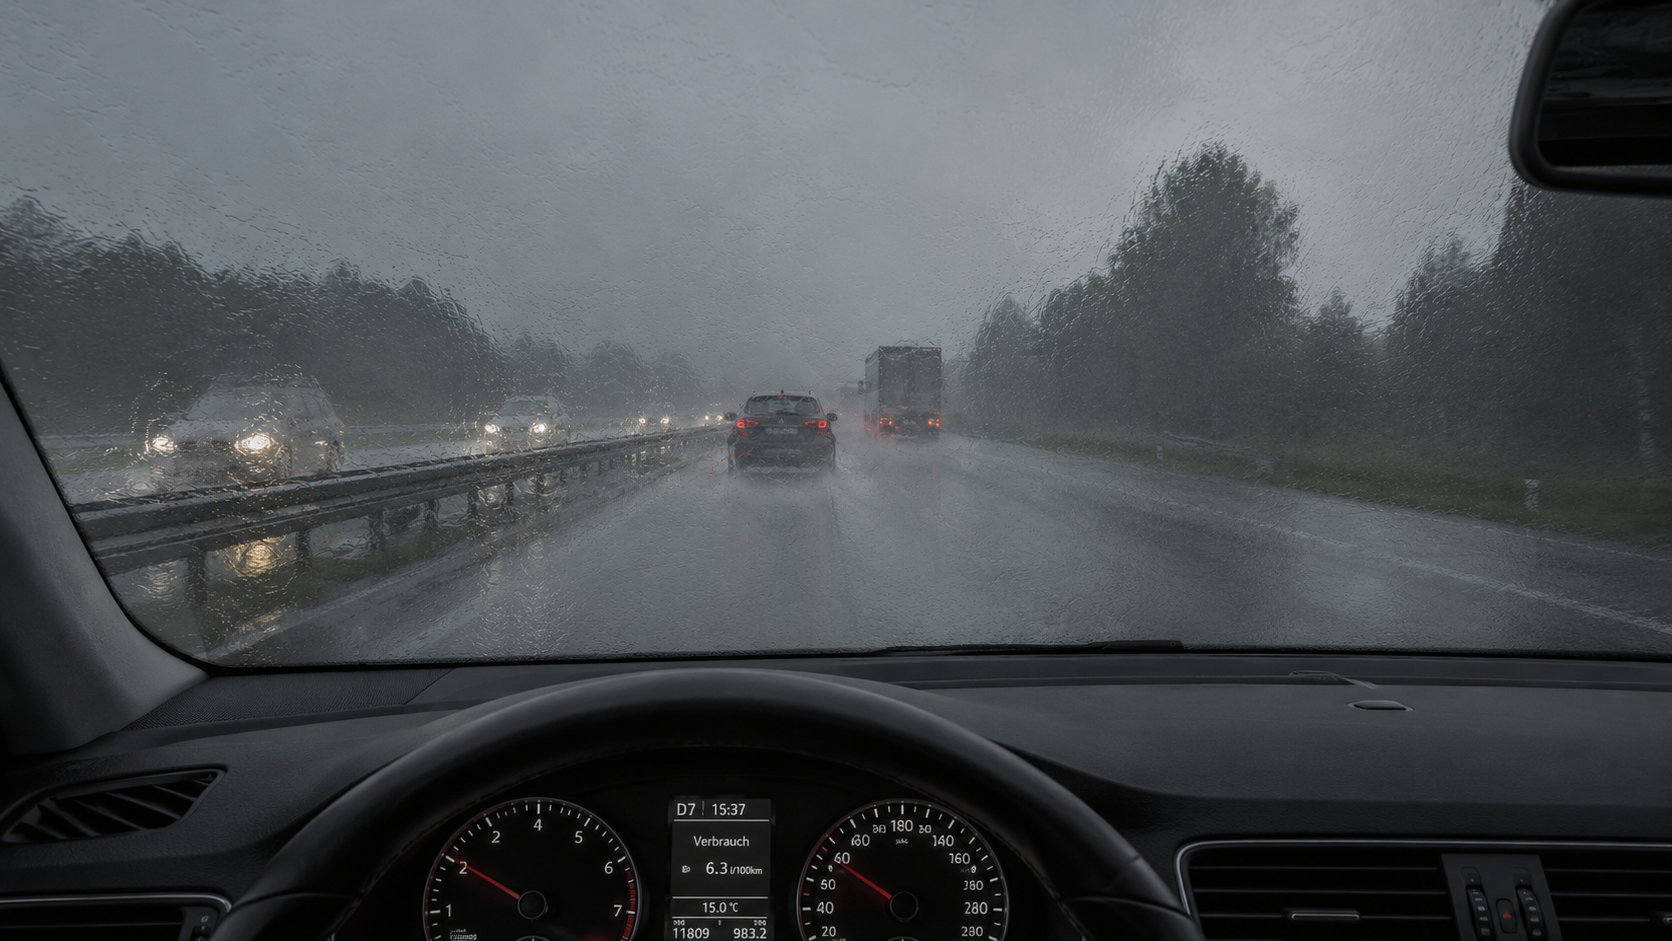
\includegraphics[width=0.5\textwidth]{images/appendix/Grenzsituation.png}
    \caption{Illustration einer möglichen Grenzsituation für eine Spurhalteassistenz}
    \label{fig:grenzsituation}
    \medskip
    {\footnotesize Bild wurde mithilfe eines Bildgenerators erzeugt.}
\end{figure}

\paragraph*{Mögliche Nachfragen}

\begin{itemize}
    \item Sollte das Fahrzeug vorher erklären, dass dies eine
          problematische Situation sein kann?
    \item Sollte das Fahrzeug während der Fahrt einen Hinweis geben?
    \item Wie deutlich müsste dieser Hinweis sein?
    \item Welche Information wäre in dieser Situation hilfreich und
          was wäre zu viel oder störend?
\end{itemize}


\subsubsection{Vertrauen, Unsicherheit und Verantwortung}

\paragraph*{Hauptfragen}

\begin{enumerate}
    \item Wann würdest Du sagen, dass Du einem Assistenzsystem vertraust?

    \item Was müsste passieren, damit dein Vertrauen in ein solches
          System sinkt?

    \item Kann es aus deiner Sicht passieren, dass man einem
          Assistenzsystem zu sehr vertraut?

    \item Was müsste ein Fahrzeug tun, damit Fahrer*innen ihre eigene
          Verantwortung nicht vergessen?
\end{enumerate}

\paragraph*{Nachfragen}

\begin{itemize}
    \item Sollte das Fahrzeug regelmäßig daran erinnern, dass man
          aufmerksam bleiben muss?
    \item Wann wären solche Erinnerungen hilfreich?
    \item Wann wären sie nervig oder störend?
    \item Sollte das System eher vorsichtig warnen oder nur in wirklich
          kritischen Situationen?
\end{itemize}


\subsubsection{Erwartungen an ein gutes Onboarding}

\paragraph*{Hauptfragen}

\begin{enumerate}
    \item Angenommen, Du bekommst ein Auto mit einer neuen
          Assistenzfunktion. Wie würdest Du dir wünschen, dass diese
          Funktion erklärt wird?

    \item Welche Informationen sollten vor der ersten Nutzung
          vermittelt werden?

    \item Welche Informationen sollten erst während der Nutzung
          erscheinen?

    \item Welche Informationen sollten nach einer kritischen Situation
          erklärt werden?

    \item Welche Form wäre für dich am hilfreichsten?

    \begin{itemize}
        \item Text
        \item Bild
        \item kurze Animation
        \item Video
        \item Sprachhinweis
        \item Anzeige im Fahrzeugdisplay
        \item HUD/visueller Hinweis
        \item App vor der Fahrt
        \item interaktives Tutorial
    \end{itemize}
\end{enumerate}

\paragraph*{Nachfragen}

\begin{itemize}
    \item Möchtest Du lieber geführt werden oder selbst erkunden?
    \item Sollte das Onboarding kurz und verpflichtend sein?
    \item Sollte man es später erneut aufrufen können?
    \item Sollte das System den Wissensstand der Nutzer*innen
          berücksichtigen?
    \item Sollte es unterschiedliche Detailstufen geben?
\end{itemize}


\subsubsection{Bewertung konkreter Onboarding-Ideen}

\paragraph*{Einleitung}

Ich nenne dir nun einige mögliche Formen von Onboarding. Bitte sage mir
spontan, ob Du diese hilfreich, störend oder unnötig finden würdest.

\paragraph*{Idee 1: Kurze Vorab-Erklärung im Fahrzeugdisplay}

Vor der ersten Nutzung erklärt das Fahrzeug in wenigen Schritten, was
die Funktion kann, wie sie aktiviert wird und wo ihre Grenzen liegen.

\textbf{Fragen:}

\begin{itemize}
    \item Wäre das hilfreich?
    \item Was müsste darin unbedingt vorkommen?
    \item Wie lang dürfte so eine Erklärung maximal sein?
\end{itemize}

Dieses Bild zeigt eine mögliche Umsetzung:

\begin{figure}[ht]
    \centering
    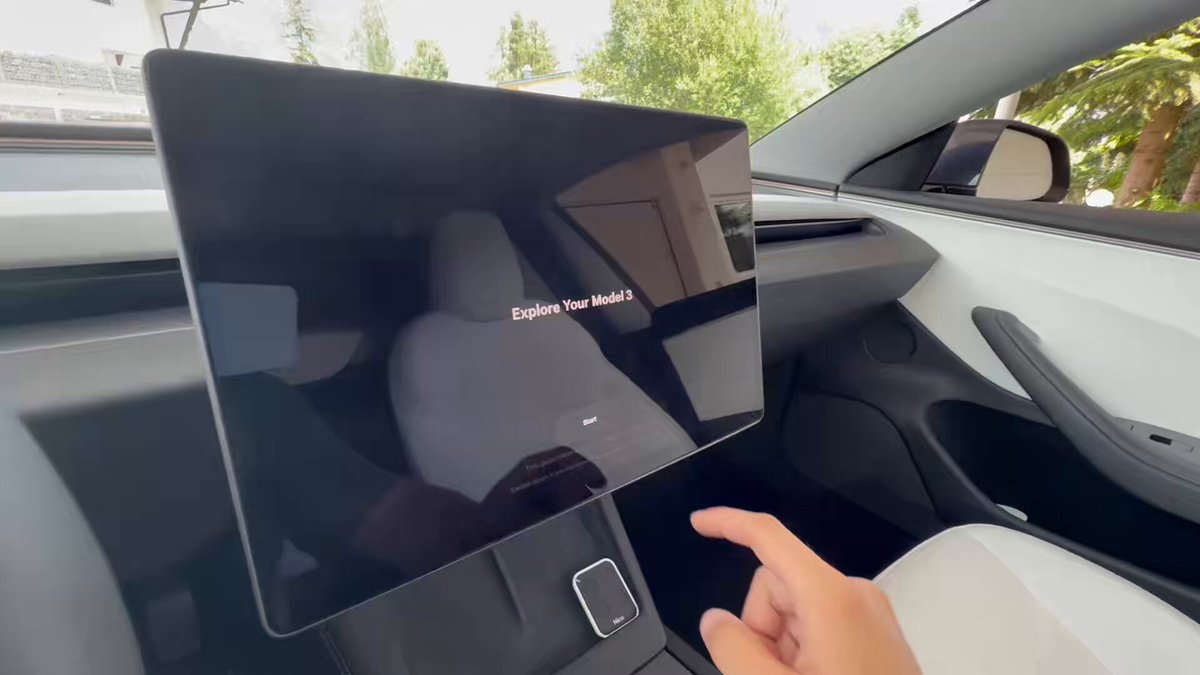
\includegraphics[width=0.5\textwidth]{images/appendix/Onboarding_Beispiel_Zuvor.jpg}
    \caption{Illustration eines Onboardings vor Fahrtantritt in einem Tesla Model 3}
    \label{fig:onboarding_zuvor}
    \medskip
    {\footnotesize Quelle: x.com/TeslaNewswire}
\end{figure}


\paragraph*{Idee 2: Situationsbezogene Hinweise während der Fahrt}

Während der Fahrt erscheint ein kurzer Hinweis, wenn eine Situation
für die Assistenzfunktion relevant wird, z.\,B.
``Toten Winkel überprüfen und in den Rückspiegel schauen''.

\textbf{Fragen:}

\begin{itemize}
    \item Wäre so ein Hinweis hilfreich?
    \item In welchen Situationen wäre er besonders wichtig?
    \item Wann wäre er störend?
\end{itemize}

Dieses Bild zeigt eine weitere mögliche Umsetzung:

\begin{figure}[ht]
    \centering
    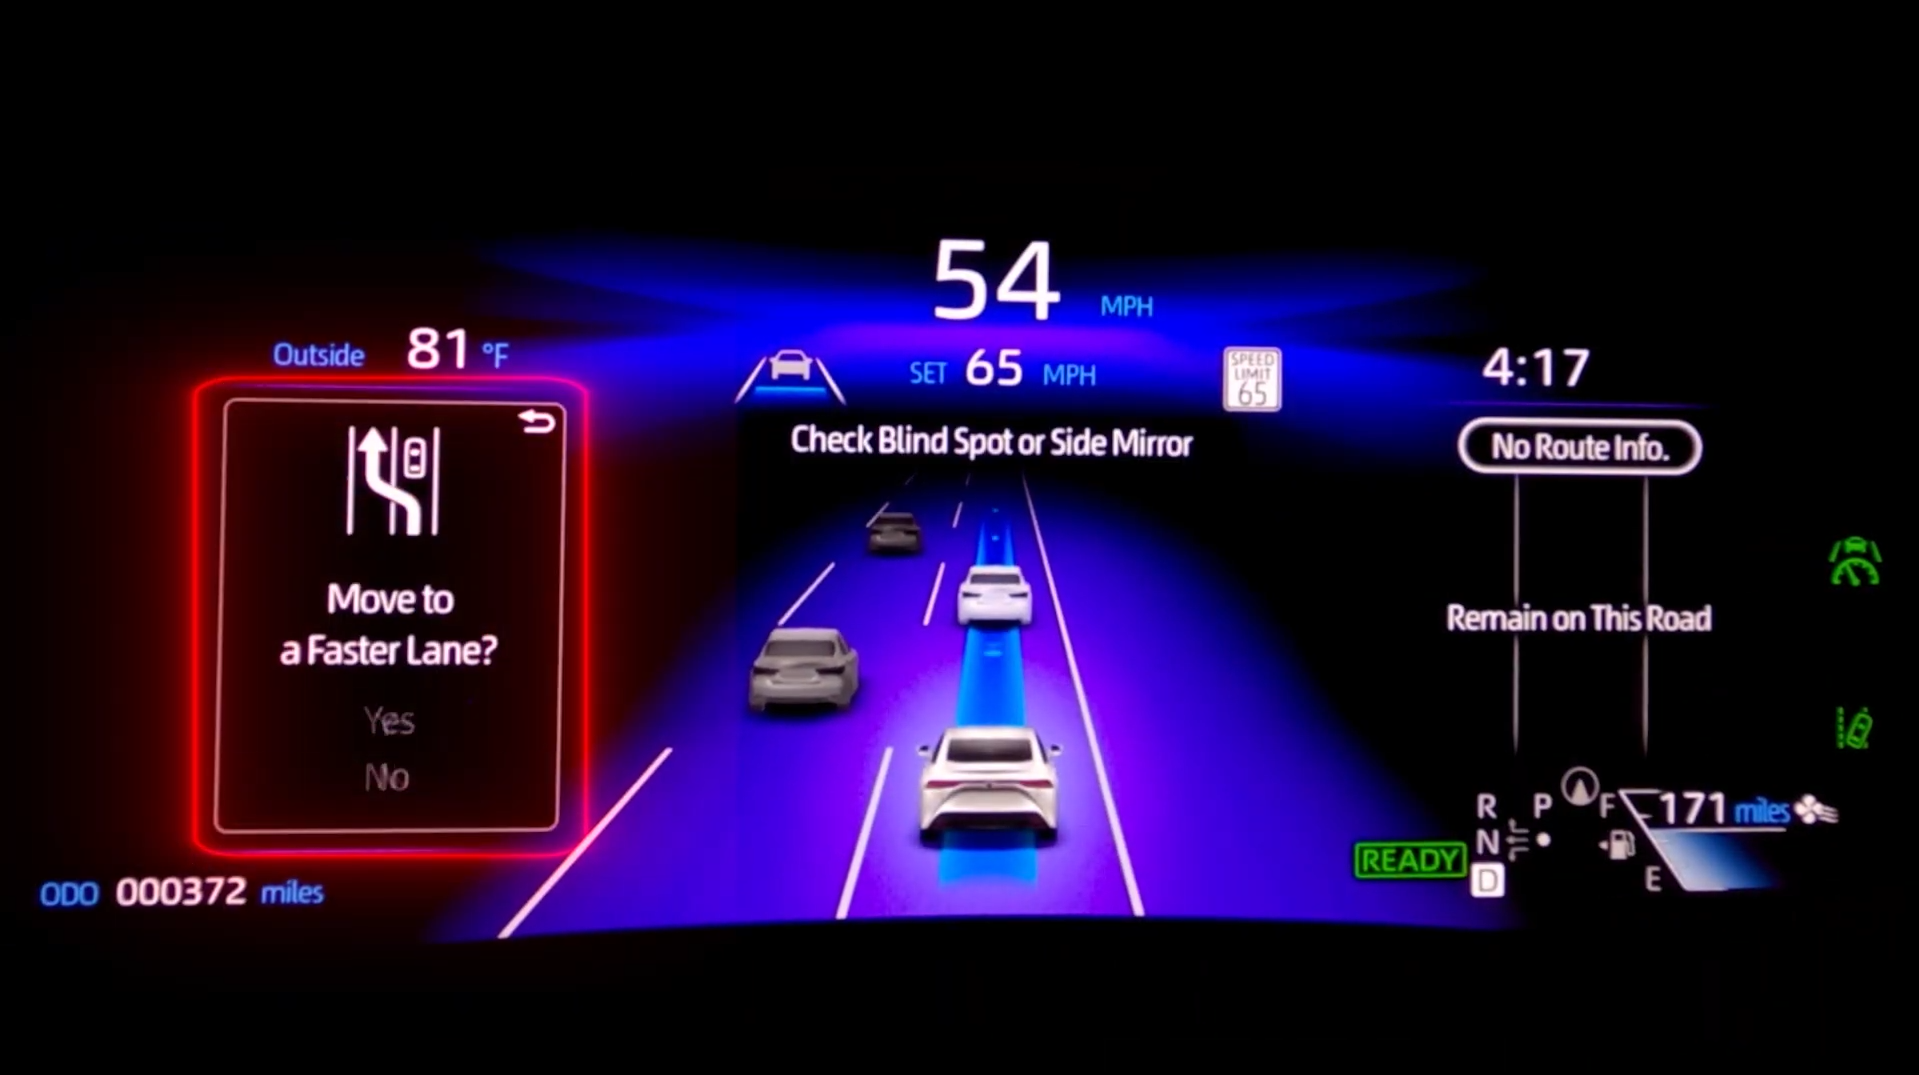
\includegraphics[width=0.5\textwidth]{images/appendix/Onboarding_Beispiel_Kontext.png}
    \caption{Illustration von kontextspezifischen Hinweisen eines Assistenzsystems während der Fahrt}
    \label{fig:onboarding_kontext}
    \medskip
    {\footnotesize Quelle: youtube.com/@toyotausa}
\end{figure}

\subsubsection{Abschlussfragen}

\paragraph*{Hauptfragen}

\begin{enumerate}
    \item Gibt es etwas, das wir bisher nicht angesprochen haben,
          das dir aber wichtig erscheint?
\end{enumerate}


\clearpage
% ============================================================
% Interviewtranskripte
% ============================================================

\section{Interviewtranskripte}
\label{sec:interviewtranskripte}

% ============================================================
% PROBAND*IN 1
% ============================================================

\subsection{Transkript Proband*in 1}
\label{subsec:transkript-p1}

\interviewerin
In diesem Gespräch geht es darum, wie Fahrer Assistenzsysteme, z. B.
einen Spurhalteassistenten, im Auto verstehen und nutzen. Es gibt keine
richtigen oder falschen Antworten. Mich interessiert vor allem, welche
Erfahrungen, Unsicherheiten oder Probleme bei der Nutzung solcher
Systeme auftreten können. Dabei geht es nicht darum, dein Fahrverhalten
zu bewerten, sondern Anforderungen an bessere Erklärungen und
Onboarding-Konzepte abzuleiten. Welche Assistenzsysteme kennst du
grundsätzlich?

\probandin{1}
Ich habe eigentlich kaum welche in meinem Auto, aber ich habe schon mal
von welchen gehört.

\interviewerin
Welche?

\probandin{1}
ABS, Spurhalteassistent, Rückfahrassistent…

\interviewerin
Aber die kennst du, mit Ausnahme vom ABS, primär von anderen Autos?

\probandin{1}
Ja.

\interviewerin
Okay, wie würdest du denn deine Erfahrung mit solchen Systemen
einschätzen? Keine Erfahrung, wenig Erfahrung, gelegentliche oder
regelmäßige Nutzung?

\probandin{1}
Eher wenig.

\interviewerin
Gäbe es denn jetzt ein Assistenzsystem, das du gar nicht benutzen
würdest, selbst wenn du es hättest?

\probandin{1}
Das fällt mir schwer zu beantworten.

\interviewerin
Erinnerst du dich an eine Situation, in der du ein Fahrassistenzsystem
zum ersten Mal genutzt hast?

\probandin{1}
Nein, nicht wirklich.

\interviewerin
Okay, dann frage ich anders. Erinnerst du dich denn, wie du
herausgefunden hast, wie das funktioniert?

\probandin{1}
Ich gucke immer in die Anleitung.

\interviewerin
Gedruckt oder digital?

\probandin{1}
Gedruckt. Ich möchte immer etwas Gedrucktes haben. Das ist mir wichtig,
weil ich Sachen in Ruhe lesen möchte. Ich mag es nicht, wenn man mich
hetzt! Es wäre auch okay, wenn mir das jemand persönlich erklärt.

\interviewerin
Wenn du jetzt mal an irgendein Assistenzsystem denkst: Was müsste man
deiner Meinung nach denn wissen, um das sicher nutzen zu können?

\probandin{1}
Bevor ich das beantworte: Mir fällt gerade noch ein, dass es so einen
Assistenten gibt, der automatisch bremst, bevor ein Unfall passiert.
Das würde ich befürworten!

\interviewerin
Aber zurück zu meiner Frage: Was müsste man denn deiner Meinung nach
wissen, um ein solches System sicher nutzen zu können?

\probandin{1}
Na ja, dass ich das halt ordentlich erklärt bekomme. Ich will wissen,
was auf mich zukommt, wenn ich zu nah auffahre.

\interviewerin
Und was denkst du, woran du erkennen würdest, ob das System gerade
aktiv ist?

\probandin{1}
Ich habe ja keine Erfahrung damit, aber ich würde mich da vielleicht
auf ein akustisches Signal verlassen.

\interviewerin
Einen Piepton meinst du?

\probandin{1}
Ja, genau.

\interviewerin
Wäre dir auch wichtig, dass das System sagt, was es tut und was du
weiterhin tun musst?

\probandin{1}
Das wäre mir auch sehr wichtig! Ich weiß das manchmal nicht und kann
das nicht erkennen.

\interviewerin
Hattest du schon mal den Fall, dass du nicht wusstest, warum eine
Assistenz bestimmte Sachen tut?

\probandin{1}
Ähm, wenn man bei Glatteis anfährt und die Räder ungleichmäßig
anziehen, hat sich das ABS komisch verhalten. Da kam dann so ein Symbol.

\interviewerin
Gibt es auch bestimmte Situationen, in denen du sagst, da vertraue ich
einem Fahrassistenzsystem auf gar keinen Fall?

\probandin{1}
Oh, da wüsste ich spontan nicht, was ich darauf antworten könnte.

\interviewerin
Sind dir bestimmte Grenzen von Assistenzsystemen bekannt? Hast du dazu
vielleicht etwas in den Medien erfahren?

\probandin{1}
Nein, ehrlich gesagt nicht.

\interviewerin
Okay, damit haben sich ein paar Folgefragen erübrigt. Lass uns mal
zusammen ein Szenario betrachten. Ich habe dir hier ein Bild
mitgebracht. Kannst du erkennen, was dort zu sehen ist?

\probandin{1}
Es ist neblig, diesig, viel Regen. Man erkennt nichts mehr auf der
Fahrbahn.

\interviewerin
Wenn du jetzt mit einem Spurhalteassistenten da langfahren würdest:
Glaubst du, das könnte problematisch sein?

\probandin{1}
Nein, das glaube ich eigentlich nicht. Ich glaube, dass die das schon
sicher erkennen.

\interviewerin
Und wenn der Assistent das jetzt nicht könnte – würdest du dir
wünschen, dass er dir sagt: Es besteht ein Problem, übernimm du bitte
das Steuer?

\probandin{1}
Ja, das ist schon sinnvoll.

\interviewerin
Und wie deutlich müsste der Hinweis sein?

\probandin{1}
Am besten auch hier ein Piepton.

\interviewerin
Noch mehr als das, oder wäre dir das zu viel?

\probandin{1}
Nein, der reicht völlig.

\interviewerin
Wann würdest du denn sagen, dass für dich der Punkt erreicht wäre, ab
dem du einem Assistenzsystem vertraust?

\probandin{1}
Ich glaube nicht, dass das passieren wird. Das ist gut ausentwickelt.

\interviewerin
Was müsste denn passieren, damit du einem Assistenzsystem nicht mehr
vertraust?

\probandin{1}
Wenn es ruckeln würde oder ich mich erschrecken würde.

\interviewerin
Glaubst du auch, dass manche Leute Assistenzsystemen zu viel vertrauen?

\probandin{1}
Ja, auf jeden Fall.

\interviewerin
Glaubst du, dass das Fahrzeug vielleicht auch etwas tun müsste, damit
der Fahrer versteht: Ich bin nicht aus meiner Verantwortung entlassen?

\probandin{1}
Darauf müsste hingewiesen werden.

\interviewerin
Okay, jetzt stell dir mal vor, du würdest ein neues Auto kaufen. Was
würdest du dir denn wünschen, was vor der ersten Fahrt in Bezug auf
Assistenzsysteme mitgeteilt werden müsste?

\probandin{1}
Ich möchte das alles vor Ort von einem Verkäufer erklärt bekommen. Das
war bei meinem Tiguan vor 14 Jahren auch so. Der soll mir erklären,
wie ich alles im Auto benutze.

\interviewerin
Okay, wenn es die Möglichkeit gäbe, dass die Erklärungen direkt in das
Auto eingebaut wären: In welcher Form würdest du dir diese wünschen?
Es könnten z. B. Texte, Videos, Animationen oder vielleicht gesprochene
Texte sein.

\probandin{1}
Also dann Text oder akustisch.

\interviewerin
Soll das System dich dann durch die Einführung leiten? Oder möchtest du
lieber selbst erkunden?

\probandin{1}
Ich möchte geführt werden. Aber ich will mir das später noch mal in
Ruhe angucken können.

\interviewerin
Okay, dann zeige ich dir jetzt noch mal zwei Bilder. Das erste Bild
zeigt eine Einführung über ein Display im Auto. Das würde man vor
Fahrtantritt machen. Das zweite Bild zeigt situationsbezogene Hinweise
während der Fahrt. Die könnte man z. B. direkt in die Windschutzscheibe
projizieren. Gibt es dahingehend eine Lösung, die für dich direkt
durchfällt?

\probandin{1}
Also das Display ist mir zu groß. Das ist ja immer noch ein Auto. Wenn
es kleiner wäre, fände ich das okay.

\interviewerin
Das ist nur ein Beispiel. Das kann man natürlich auch kleiner machen.
Was ist denn mit der zweiten Variante?

\probandin{1}
Also… Ich weiß nicht. Das wäre schon gut, aber es darf nicht meine
Sicht behindern.

\interviewerin
Okay, dann ist meine letzte Frage, ob es noch irgendetwas gibt, was du
mir mitteilen willst. Habe ich etwas nicht angesprochen, was dir
wichtig ist?

\probandin{1}
Also ich habe noch mal über den Notbremsassistenten nachgedacht.
Funktioniert der bei jeder Geschwindigkeit gut?

\interviewerin
Nein, das würde ich so nicht sagen. Auch der Assistent kann nichts an
einem sehr langen Bremsweg bei hohen Geschwindigkeiten ändern. Er ist
aber dennoch für moderne Fahrzeuge sehr wichtig.

\probandin{1}
Das zeigt ja noch mal, dass man sich dann besser doch nicht zu
100~\% darauf verlassen sollte.


% ============================================================
% PROBAND*IN 2
% ============================================================

\clearpage
\subsection{Transkript Proband*in 2}
\label{subsec:transkript-p2}

\interviewerin
In diesem Gespräch geht es darum, wie Fahrer Assistenzsysteme, z. B.
einen Spurhalteassistenten, im Auto verstehen und nutzen. Es gibt keine
richtigen oder falschen Antworten. Mich interessiert vor allem, welche
Erfahrungen, Unsicherheiten oder Probleme bei der Nutzung solcher
Systeme auftreten können. Dabei geht es nicht darum, dein Fahrverhalten
zu bewerten, sondern Anforderungen an bessere Erklärungen und
Onboarding-Konzepte abzuleiten. Welche Assistenzsysteme kennst du
grundsätzlich?

\probandin{2}
Der Witz ist ja: Man benutzt schon einige und weiß es gar nicht oder ist
stark daran gewöhnt. ABS, ASR, Spurassistent, Limiter,
Geschwindigkeitsregelautomat, sprich Tempomat, Müdigkeitsassistent,
theoretisch sogar die aktiven Scheinwerfer. Im Prinzip ist es die halbe
Elektronik.

\interviewerin
Welche dieser Assistenzsysteme hast du selbst schon genutzt?

\probandin{2}
Alles, was ich aufgezählt habe.

\interviewerin
In welchem Kontext hast du sie genutzt? Beispielsweise eigenes Auto,
Mietwagen, Firmenwagen …

\probandin{2}
Firmenwagen. Das ist ja aufgrund der Nutzungsbestimmungen in der Firma
auch mein Privatauto. Auch Mietwagen kann man hier sicherlich nennen.

\interviewerin
Wie würdest du denn deine eigene Erfahrung mit Fahrassistenzsystemen
einschätzen? Keine Erfahrung, wenig Erfahrung, gelegentliche oder
regelmäßige Nutzung?

\probandin{2}
Regelmäßig.

\interviewerin
Gibt es ein System, das du besonders gerne benutzt?

\probandin{2}
Ja, den Limiter. Wer wie ich immer viel fährt, will die teuren Fotos
vermeiden. Ist auch für Baustellen extrem gut. Spurhalteassistenz hasse
ich dafür wie die Pest.

\interviewerin
Warum?

\probandin{2}
Der ist einfach übergriffig und vor allen Dingen verhindert er
teilweise eben eigenes Reagieren. Meiner Meinung nach ist auch die
Fehlerquote zu hoch. Bei langsamem Überholen etc. reagiert er komisch,
habe ich festgestellt. Ich habe jetzt übergangsweise einen Dacia statt
meines Kuga gefahren. Hat ein paar Features mehr … Katastrophe! Das ist
kein Auto mehr, das ist ein Haufen Gimmicks.

\interviewerin
Wie darf ich das verstehen? Hast du das Gefühl, dich erreichen zu viele
Informationen und davon ist nur ein Bruchteil relevant, sodass man sich
nicht mehr auf die Hauptaufgabe, das Fahren, konzentrieren kann?

\probandin{2}
So ist es.

\interviewerin
Gibt es auch ein Assistenzsystem, das du bewusst nicht benutzt?

\probandin{2}
Spurhalteassistenz. Das ist wirklich grausig. Extrem wichtig ist der
Müdigkeitsassistent, weil jeder sich da wahrscheinlich in die Tasche
lügt, was die eigene Fahrtüchtigkeit angeht. Dementsprechend sollte man
das zumindest infrage stellen.

\interviewerin
Okay, die nächste Frage ist, ob du ein Assistenzsystem auch schon mal
ausgeschaltet hast. Ich nehme an, die Spurhalteassistenz ist davon
betroffen, weil du zuvor gesagt hast, dass sie dich stört.

\probandin{2}
So ist es.

\interviewerin
Ich weiß nicht, ob du dich noch an die Situation erinnerst, in der du
zum ersten Mal ein Fahrassistenzsystem genutzt hast. Wie hast du damals
herausgefunden, wie das System funktioniert?

\probandin{2}
Na ja, Anti-Schlupf-Regelung, Anti-Blockier-System … Das waren ja die
ersten Systeme. Ich habe sie ausprobiert. Im Prinzip habe ich sie also
durch Praxis gelernt. Das hat mir Sicherheit gegeben, dass ich mich auf
diese Systeme verlassen konnte. Das wäre aus meiner Sicht dumm, in
diesem Fall eine eigene Entscheidung treffen zu wollen. Das sind
Systeme, die angenehm unterstützen. Aber der Spurhalteassistent … Wie
gesagt, der nervt mich.

\interviewerin
Gibt es irgendetwas, was du vor der Nutzung konsultiert hast, also z. B.
eine Bedienungsanleitung? Oder vielleicht einen Händler bei Neuwagen?

\probandin{2}
Beides im Prinzip. Die Erklärung beim Händler ist aber zu schwach.
Leider Gottes sind die Autohäuser heute zunehmend konzentriert, sprich:
immer weniger Fachhändler. Die können trotzdem immer weniger erklären
beziehungsweise erklären „Verkaufsfeatures“, aber sie bringen dir nicht
die wirklichen Vorteile oder eben das Verhalten des Autos bei. Was ist
für mich wichtig? Was ich immer vermisse, ist: Die sollten mal eine
Runde mit dir drehen und Sachen ausprobieren, die das Auto kann. Dafür
nimmt sich kein Mensch mehr Zeit. Das wäre aber eigentlich Lernen anhand
der Praxis, bei dem du registrierst, wie die Dinger funktionieren. Es
geht nur noch um den Verkauf, und die kennen die Grenzen dieser Systeme
oft selbst nicht.

\interviewerin
Würdest du auch in Betracht ziehen, dich über YouTube oder eine App zu
informieren?

\probandin{2}
Ja, vor allem bei den Assistenten, die unbemerkt eingreifen. Bei den
kritischen würde ich immer bevorzugen, es selbst auszuprobieren.

\interviewerin
Wenn du an ein Assistenzsystem wie die Spurhalteassistenz oder einen
Tempomaten denkst: Was muss man deiner Meinung nach wissen, um das
sicher nutzen zu können?

\probandin{2}
Man muss wissen, wie das Auto reagiert. Wenn das Auto anfängt, anders
zu reagieren, als man es kennt, könnte man durch die eigenen Reaktionen,
auch unbewusste Reaktionen, Fehler machen, die man sonst nicht macht.
Sprich: Lenkrad rumreißen, dagegenhalten, und dann dreht das Auto sich
quer. Da gibt es ja alle möglichen unpassenden Verhaltensweisen, die du
machen kannst. Vollgas beim Heckantrieb, dann bricht das Auto aus und du
machst Bekanntschaft mit der Leitplanke. Ich glaube, ich fahre zu viel.
Ich habe einfach zu viel gesehen.

\interviewerin
Und woran erkennst du, dass ein Assistenzsystem gerade aktiv ist?

\probandin{2}
In der Regel wird es in der Konsole angezeigt. Wenn du aktiv gucken
willst, ob es an ist oder nicht, siehst du es. Aber du hast einfach
keinen Überblick mehr. Weil zu viele Lämpchen an sind, sind es einfach
zu viele Informationen. Du guckst nur noch ins Display, wenn du etwas
wirklich wissen willst. Es ist nicht mehr so, dass das Display dir
vermittelt, wo du dich gerade befindest.

\interviewerin
Das heißt, du hast auch Probleme damit, manchmal zu erkennen, was das
System jetzt gerade oder zukünftig tun wird, weil du auch nur die
Systemzustände …

\probandin{2}
Richtig, das zeigt dir ja auch kein Display an. Das Display zeigt dir
nicht an: Das Auto zieht jetzt nach rechts.

\interviewerin
Gab es auch eine bestimmte Situation, in der du nicht verstanden hast,
warum ein Assistenzsystem so reagiert hat, wie es reagiert hat?

\probandin{2}
Ja, das war ganz normal bei einem Überholvorgang, bei dem der
Spurhalteassistent anfängt, in eine bestimmte Richtung zu ziehen. Ich
hatte das Gefühl, dass ich aktiv dagegenarbeiten muss. Man hat das
Gefühl, man muss um die Autorität im Auto kämpfen.

\interviewerin
Das heißt, gerade in komplizierten Situationen, beispielsweise bei
einem Überholvorgang, würdest du sagen, dass du dem Assistenzsystem
nicht vertraust?

\probandin{2}
Ja, ein völliger Killing-Fact, weil da unbewusste Reaktionen tödlich
sein können. Mit Training ja, ohne Training nie und nimmer. Und da muss
man es auch ausschalten können, weil das nicht jeder mag. Generell bin
ich bei Assistenzsystemen der Meinung: Wenn man das Spektakel übertreibt,
verlernen die Leute das Fahren und damit auch, die Verantwortung für
das Auto zu übernehmen.

\interviewerin
Sind dir bestimmte Grenzen von Fahrassistenzsystemen bekannt, und wie
hast du diese kennengelernt?

\probandin{2}
Na ja, die Klassiker von Tesla aus den Medien. Das sind Fälle, bei denen
auf Kreuzungen teilweise Leute beim Autopiloten ums Leben gekommen
sind. Und da befinden wir uns natürlich in einem Grenzbereich. Wie sagt
Tesla immer? Da kommen weniger Leute ums Leben als beim Fahren ohne
Assistent. Aber das ist eine relativ makabere Statistik, würde ich
sagen.

\interviewerin
Wenn du an deine eigenen Erfahrungen mit Grenzen denkst: Wie hast du in
einer solchen Situation reagiert?

\probandin{2}
Ich kann mir vorstellen, dass bei Leuten in bestimmten Situationen
Panik entstehen kann, wenn die nicht erfahren genug sind. Das heißt,
wenn die noch relativ jung sind oder nicht viel fahren … Also ein
Klassiker ist auch, dass man auf der Autobahn unterwegs ist und bei
anderen Fahrern der Spurhalteassistent aktiv ist. Wenn der in eine
bestimmte Richtung zieht, sind die oft völlig überfordert. Ich selbst
fahre 70.000 Kilometer im Jahr. Da bist du routiniert, du kennst
Glatteis, du kennst Sachen, bei denen du nicht auf die Bremse trittst.
Das sind eigentlich Sachen, die lernst du halt mit einer Million
Kilometer. Sonst überlebt man da draußen nicht, das ist ganz einfach.

\interviewerin
Das heißt, dich selbst wirft eine Grenzerfahrung nicht so schnell aus
der Bahn?

\probandin{2}
Nein, mich nervt es, aber es schmeißt mich nicht aus der Bahn.

\interviewerin
Ich möchte dir ein Bild präsentieren. Auf dem Bild siehst du eine sehr
regnerische Szene, bei der die Fahrbahnmarkierungen nicht mehr gut zu
erkennen sind. Wenn du dir vorstellst, dort mit aktivierter
Spurhalteassistenz unterwegs zu sein: Glaubst du, dass das ein Problem
sein könnte?

\probandin{2}
Klar.

\interviewerin
Und würdest du dir wünschen, dass das Fahrzeug vor Fahrtantritt
ankündigt, dass das ein Problem sein könnte?

\probandin{2}
Nein, ich würde mir wünschen, dass der Assistent sich während der Fahrt
abschaltet. Das muss er natürlich kommunizieren, damit man sich nicht
auf etwas verlässt, was nicht da ist. Was nicht passieren darf, ist,
dass er wie eine KI eingreift und selbstständig Dinge entscheidet.
Wenn die Gegebenheiten nicht stimmen, macht der Assistent mehr Fehler
als ein Mensch. Dann ist es kein Assistent mehr, dann ist es ein Risiko.

\interviewerin
Wie deutlich soll der Hinweis gestaltet sein?

\probandin{2}
Also Alarmtöne sind eine Katastrophe. Man sollte einen Sprachassistenten
in Erwägung ziehen, der ruhig darauf hinweist. Deutlich, aber immer
ruhig. Ich hasse es, wenn es ständig piepst. Du hast keinen Fokus mehr,
du ärgerst dich und du fährst unsicher. Das ist meiner Meinung nach eine
Katastrophe. Das hilft nicht, das macht unsicher.

\interviewerin
Gibt es für dich eine Schwelle, ab der du einem Assistenzsystem
vertraust?

\probandin{2}
Im Bereich Stadtverkehr würde ich das sogar begrüßen, weil es relativ
komplexe Situationen gut erfasst hat. Du musst aber das letzte Wort
haben können, du musst ihn überstimmen können, damit er korrigiert
werden kann, wenn er irgendwas falsch macht. Darauf müssen die Leute
auch trainiert sein. Sie dürfen sich nicht darauf verlassen, sonst sind
sie nur noch Beifahrer. Auf Autobahnen und je höher die Geschwindigkeit
ist, desto weniger würde ich ihm trauen, einfach weil eine
Fehleinschätzung dann tödlich sein könnte.

\interviewerin
Was würde dazu führen, dass dein Vertrauen in Assistenzsysteme sinkt?

\probandin{2}
Sagen wir mal so: Es wird nur über Fehler und Fehlerbehebung gehen.
Sonst hätten wir heute noch kein System. Mir ist wichtig, dass eine
Assistenz eine Assistenz bleibt. Sobald die richtig ins Fahren
eingreift, wird es kritisch. Dann sollte sie so sicher wie möglich sein.
Denn da sind die Fehler einfach tödlich.

\interviewerin
Glaubst du, dass es auch Personen gibt, die einer Assistenz zu sehr
vertrauen? Du hast ja eben schon die Unfälle bei Tesla angesprochen.

\probandin{2}
Das war genau der Punkt, an dem ich sagte: Wir werden dann Leute haben,
übertrieben gesagt, die wie Zombies Auto fahren. Dann kannst du auch
direkt Taxi fahren. Wenn dann etwas passiert, wird die Verantwortung
letztendlich nie das System haben. Die letzte Verantwortung wird von
Gesetzes wegen immer der Fahrer haben. Und dann hat er eigentlich nicht
mehr die Mittel, die Möglichkeiten und auch nicht mehr das Wissen,
dieser Verantwortung gerecht zu werden. Und das ist eigentlich fast
noch das Schlimmere an der Sache.

\interviewerin
Sollte das Fahrzeug auch regelmäßig den Fahrer an die eigene
Verantwortung erinnern?

\probandin{2}
Ich glaube, das ist darüber nicht zu regeln, weil das irgendwann den
gleichen Nervfaktor haben wird. Das heißt, die Leute werden versuchen,
das auszustellen oder es ignorieren. Sie werden aber nicht die
Verantwortung wahrnehmen. Das wird meiner Meinung nach nur über die
Praxis gehen, sodass man die Grenzen kennenlernt.

\interviewerin
Ich halte es für sinnvoll, je mehr Fahrassistenten wir haben, auch
regelmäßig Fahrsicherheitstrainings zu machen – und zwar mit
Assistenten.

\probandin{2}
Das würde zum einen helfen, die Assistenzsysteme besser zu nutzen. Auf
einem abgesperrten Gelände könnte das klappen, wie zum Beispiel beim
Nürburgring durch den ADAC. Es ist aber auch ein Unterschied, wenn ein
trainierter Coach die Leute an die Grenzen führt, sodass sie das durch
die Erfahrung mit der Grenze deutlich besser behalten als irgendeine
Warnung. Meiner Meinung nach müssen die auch mal bewusst die Grenze
überschreiten, weil das tiefergehend verarbeitet wird. Das ist einfach
eine Erfahrung, die die Leute behalten.

\interviewerin
Dann kommen wir jetzt zum Schluss noch zu deinen Erwartungen, wie man
Onboarding-Systeme für Assistenzfunktionen gestalten könnte. Angenommen,
du bekommst ein Auto mit einer neuen Assistenzfunktion. Wie würdest du
dir wünschen, dass diese Funktion erklärt wird? Was würdest du sagen,
muss vor der ersten Nutzung vermittelt werden, was während der Nutzung
und was vielleicht im Anschluss an eine kritische Situation?

\probandin{2}
Es ist schon wichtig, dass es als Ergänzung zu einer Probefahrt eine
Bedienungsanleitung gibt, in der man Sachen nachschlagen kann. Das kann
man heutzutage auch mit Apps oder Ähnlichem machen, weil das
wahrscheinlich besser funktioniert. Insbesondere bei den Sachen, die
wirklich eingreifen.

\interviewerin
Was ist mit einer Anleitung, die in die Systeme eines Fahrzeugs
integriert ist, z. B. in ein Fahrzeugdisplay?

\probandin{2}
Auf jeden Fall ist das auch eine Lösung. Die meisten Leute – wir haben
heute viele Digital Natives – wachsen damit anders auf. Dann
registrieren die das auch.

\interviewerin
Würdest du dabei lieber geführt werden oder würdest du das lieber
selbst erkunden?

\probandin{2}
Das sollte man eigentlich als Option offenlassen, weil es verschiedene
Typen gibt. Ich persönlich würde das lieber selbst steuern wollen. Es
gibt aber unsichere Menschen, für die es wichtig ist, einen Leitfaden
zu haben. Damit kann sichergestellt werden, dass wirklich alles
abgearbeitet ist. Das liegt auch ein bisschen an der Erfahrung. Ganz
banal: Ein 18-Jähriger muss da mehr geführt werden, weil der sonst
glaubt, er kann schon alles. Und einer, der über eine Million Kilometer
gefahren ist, wie ich, kann durchaus mal gucken: Was brauche ich davon?
Was kenne ich davon?

\interviewerin
Dann zeige ich dir zum Abschluss jetzt noch zwei Bilder. Das erste Bild
zeigt die Möglichkeit, bei der ein Onboarding über ein integriertes
Display umgesetzt wurde. Dieses würde man eher vor Fahrtantritt
bedienen. Das zweite Bild zeigt kontextspezifische Erklärungen, die
z. B. in die Windschutzscheibe projiziert werden könnten. Gibt es einen
Ansatz, der für dich sofort durchfällt?

\probandin{2}
Die Idee mit der Windschutzscheibe ist hundertmal besser, weil du keine
Blickabwendung hättest. Das ist der Klassiker: Es gibt Strafen für
Handys, gleichzeitig haben wir aber die Informationen zu Systemen, zu
Fahrten und anderen Sachen auf dem Display, also ganz woanders. Das
heißt, wenn wir da hingucken, sind wir vom Verkehr weg. Im Prinzip gibt
es die Technologie ja schon im Flugverkehr. Die machen es halt nur
direkt über die Visiere. Das ist jetzt natürlich ein Beispiel, das
völlig anders ist. Aber lass uns mal ehrlich sein: Die ganzen
Entwicklungen kommen aus der Raumfahrttechnik und aus der
Militärtechnik. Waffensysteme werden halt komplett darüber gesteuert,
die mehr als, sag ich mal, empfindlich sind. Dann kann man es mit den
Autos natürlich auch so machen. Und dann hätte man da natürlich eine
große Projektionsfläche.

\interviewerin
Was wäre für dich in dem Zusammenhang zu viel? Wann würde dich die
Projektion stören?

\probandin{2}
Es darf nicht beim Fahren stören. Man müsste auch klären, wo es beim
Fahren angezeigt wird. Sprich: Der Blickwinkel muss beachtet werden.
Ich muss immer noch freie Sicht haben, und andere Sachen, die
ausführlich und raumgreifend sind, sollte man vielleicht auch nur in
einem stehenden Auto erlauben, damit der Straßenverkehr nicht gefährdet
wird.

\interviewerin
Gibt es noch etwas, was ich nicht angesprochen habe, was dir aber
wichtig erscheint?

\probandin{2}
Nein, das passt für mich so weit.


% ============================================================
% PROBAND*IN 3
% ============================================================

\clearpage
\subsection{Transkript Proband*in 3}
\label{subsec:transkript-p3}

\interviewerin
In diesem Gespräch geht es darum, wie Fahrer Assistenzsysteme, z. B.
einen Spurhalteassistenten, im Auto verstehen und nutzen. Es gibt keine
richtigen oder falschen Antworten. Mich interessiert vor allem, welche
Erfahrungen, Unsicherheiten oder Probleme bei der Nutzung solcher
Systeme auftreten können. Dabei geht es nicht darum, dein Fahrverhalten
zu bewerten, sondern Anforderungen an bessere Erklärungen und
Onboarding-Konzepte abzuleiten. Welche Assistenzsysteme kennst du
grundsätzlich?

\probandin{3}
Spurassistent, Müdigkeitssensor und Tempomat. Vom Letztgenannten bin ich
aber kein Freund. Ich habe immer das Gefühl, selbst eingreifen zu müssen.

\interviewerin
Und das hast du alles auch schon selbst genutzt?

\probandin{3}
Ja, das habe ich schon genutzt.

\interviewerin
Und was ist mit dem Kontext? Hast du das im eigenen Auto, in einem
Mietwagen oder in einem Fahrzeug von Angehörigen genutzt?

\probandin{3}
Das habe ich alles in meinem Bus, den ich zum Transport in meiner Firma
nutze.

\interviewerin
Und wenn du deine eigene Erfahrung damit einschätzen würdest? Was
würdest du sagen, trifft eher auf dich zu: keine Erfahrung, wenig
Erfahrung, gelegentliche oder regelmäßige Nutzung?

\probandin{3}
Wenig Erfahrung.

\interviewerin
Welches der Systeme benutzt du besonders gerne?

\probandin{3}
Ich habe keinen Favoriten.

\interviewerin
Gibt es ein System, das du bewusst nicht benutzt, obwohl es verfügbar
wäre?

\probandin{3}
Auch nicht.

\interviewerin
Gab es schon Situationen, in denen du ein Assistenzsystem auch mal
ausgeschaltet hast?

\probandin{3}
Nein.

\interviewerin
Wenn du jetzt versuchst, dich an die Situation zu erinnern, in der du
ein solches System zum ersten Mal genutzt hast: Wie hast du
herausgefunden, wie das System funktioniert?

\probandin{3}
Ich habe einfach Dinge ausprobiert.

\interviewerin
Hast du vor der Nutzung auch Informationen erhalten? Das können z. B.
Bedienungsanleitungen oder ein Händler sein, der ein System erklärt.

\probandin{3}
Nein.

\interviewerin
Gäbe es irgendetwas, was du dir vor der ersten Nutzung an Informationen
gewünscht hättest?

\probandin{3}
Nicht wirklich. Wenn, dann probiere ich es aus. Ich sehe auch nicht
wirklich, wie mich die Erzählungen eines Verkäufers weiterbringen
sollen. Das behält man so nicht.

\interviewerin
Was müsste man denn deiner Meinung nach wissen, um ein beispielhaftes
Assistenzsystem sicher nutzen zu können?

\probandin{3}
Ob es Grenzen hat oder so? Kann ich dir nicht wirklich sagen.

\interviewerin
Woran würdest du denn erkennen, dass ein Assistenzsystem aktiv ist?

\probandin{3}
Wahrscheinlich, weil irgendeine Lampe leuchtet. Vielleicht auch etwas
Akustisches.

\interviewerin
Hast du auch eine Idee, woran du erkennst, was das System gerade tut?

\probandin{3}
Nein.

\interviewerin
Gäbe es eine Situation, in der du dem Fahrassistenzsystem eher nicht
vertrauen würdest?

\probandin{3}
Im Stadtverkehr. Es ist unübersichtlich und man muss schnell reagieren
können. Da passieren wahrscheinlich viele Fehler.

\interviewerin
Kennst du auch Grenzen von Assistenzsystemen? Aufgrund einer
persönlichen Erfahrung oder aus den Medien?

\probandin{3}
Ja, über autonomes Fahren habe ich nichts Gutes gehört. Ich hatte den
Eindruck, dass das häufig komplett schief geht.

\interviewerin
Okay, dann zeige ich dir jetzt dieses Bild hier. Kannst du erkennen,
was auf dem Bild zu sehen ist?

\probandin{3}
Es regnet und es besteht die Gefahr von Aquaplaning.

\interviewerin
Genau. Das wäre eine problematische Situation, weil die
Spurhalteassistenz dann vielleicht nicht so gut funktioniert. Sollte
das Fahrzeug vorher erklären, dass so eine Situation problematisch sein
kann? Oder würdest du Hinweise während der Fahrt bevorzugen?

\probandin{3}
Ja, darüber sollte schon vorher aufgeklärt werden. Während der Fahrt
würde mir ein Piepton reichen.

\interviewerin
Wie deutlich müsste der Hinweis sein?

\probandin{3}
Vielleicht eine Anzeige vorne im Display.

\interviewerin
Wann würde dich das eher stören?

\probandin{3}
Wenn das jetzt dauerhaft piepen würde. Dann kriegst du irgendwann einen
Herzinfarkt.

\interviewerin
Wann würdest du sagen, ist für dich der Punkt erreicht, an dem du einem
Assistenzsystem vertraust?

\probandin{3}
Also im Moment finde ich das manchmal schon grenzwertig. Aber es müsste
sich erst bewähren.

\interviewerin
Und gäbe es etwas, was dein Vertrauen erschüttern würde?

\probandin{3}
Wenn du im Fernsehen siehst, dass da wirklich ein schwerer Unfall
passiert.

\interviewerin
Kann es aus deiner Sicht auch sein, dass man einem Assistenzsystem
vielleicht auch zu sehr vertraut?

\probandin{3}
Definitiv.

\interviewerin
Und was müsste ein Fahrzeug tun, damit der Fahrer seine eigene
Verantwortung nicht vergisst?

\probandin{3}
Man muss darauf aufmerksam machen.

\interviewerin
Sollte das System eher immer vorsichtig warnen oder nur in kritischen
Situationen?

\probandin{3}
Vorsichtig warnen.

\interviewerin
Angenommen, du würdest jetzt ein komplett neues Auto kaufen und dieses
Auto besäße eine dir noch völlig unbekannte Assistenzfunktion. Wie
würdest du dir denn wünschen, dass dir die Funktion erklärt wird?

\probandin{3}
Vielleicht über ein Video? Texte oder Bilder sind auch okay. Aber es
soll nicht mit mir reden.

\interviewerin
Möchtest du in diesem Prozess lieber geführt werden? Oder willst du
frei erkunden?

\probandin{3}
Es soll mich durchführen. Am besten sieht jeder einfach das Gleiche.

\interviewerin
Dann zeige ich dir zum Abschluss nur noch zwei Bilder. Das erste Bild
zeigt ein Display in einem Auto. Auf diesem Display kann man Eingaben
per Touch tätigen. Auf diesem Weg würden Informationen vermittelt, die
vor Fahrtantritt konsumiert werden können. Das zweite Bild zeigt eine
kontextspezifische Einblendung, die während der Fahrt erscheinen
könnte. Das würde sich beispielsweise für eine Einblendung in der
Windschutzscheibe eignen. Fällt einer der beiden Ansätze für dich
direkt durch?

\probandin{3}
Also das in der Windschutzscheibe finde ich nicht gut. Ich kann noch
nicht mal sagen, warum. Ich finde es unheimlich. Das andere ist aber
okay. Mir fällt es schwer, solche konzeptionellen Ansätze jetzt zu
bewerten.

\interviewerin
Okay, dann vertiefen wir das auch nicht weiter. Möchtest du noch etwas
ergänzen, was nicht zur Sprache kam?

\probandin{3}
Nein, alles gut.


% ============================================================
% PROBAND*IN 4
% ============================================================

\clearpage
\subsection{Transkript Proband*in 4}
\label{subsec:transkript-p4}

\interviewerin
In diesem Gespräch geht es darum, wie Fahrer Assistenzsysteme, z. B.
einen Spurhalteassistenten, im Auto verstehen und nutzen. Es gibt keine
richtigen oder falschen Antworten. Mich interessiert vor allem, welche
Erfahrungen, Unsicherheiten oder Probleme bei der Nutzung solcher
Systeme auftreten können. Dabei geht es nicht darum, dein Fahrverhalten
zu bewerten, sondern Anforderungen an bessere Erklärungen und
Onboarding-Konzepte abzuleiten. Welche Assistenzsysteme kennst du
grundsätzlich?

\probandin{4}
Also ich kenne ABS, Totwinkelassistent, autonomes Fahren generell,
Berganfahrhilfe, Müdigkeitsassistent und Einparkhilfe.

\interviewerin
Welche davon hast du selbst schon genutzt?

\probandin{4}
Also Berganfahrhilfe, ABS, Einparkhilfe und den Spurhalteassistenten.
Letzteren aber nur in einem Mietfahrzeug.

\interviewerin
Daran knüpft die nächste Frage auch an. In welchem Fahrzeugkontext hast
du diese Systeme genutzt?

\probandin{4}
Mietwagen habe ich schon erzählt. Mein eigenes Auto muss ich natürlich
auch nennen. Moment, ich fahre auch Motorrad, da gibt es so eine Art ESP
in Kurven, damit man nicht ins Schleudern gerät.

\interviewerin
Okay, kannst du dich selbst einschätzen, wie du deinen Umgang mit
Assistenzsystemen beschreiben würdest? Also keine Erfahrung, wenig
Erfahrung, gelegentliche Nutzung oder regelmäßige Nutzung?

\probandin{4}
Gelegentlich.

\interviewerin
Gibt es Systeme, die du bewusst nicht nutzt?

\probandin{4}
Ja, autonomes Fahren würde ich nicht benutzen. Da habe ich zu viel
Negatives aus den Medien darüber gehört. Das ist mir nicht geheuer.

\interviewerin
Gab es schon Situationen, in denen du ein Assistenzsystem ausgeschaltet
hast?

\probandin{4}
Also bei der Spurhalteassistenz war ich wirklich drauf und dran. Da
wird man ja komplett wahnsinnig, wenn man überholen möchte. Das macht
ja wirklich kein Mensch, da immer zu blinken. Ich habe es irgendwann
trotzdem gemacht.

\interviewerin
Erinnerst du dich an eine Situation, in der du ein
Fahrerassistenzsystem zum ersten Mal genutzt hast?

\probandin{4}
Das hatte ich eben ganz vergessen. Ich habe in der Fahrschule die
Notbremsassistenz benutzt. Da habe ich das gelernt, während ein
Fahrlehrer mit draufgeguckt hat. Die Berganfahrhilfe habe ich dann
selbst irgendwo in Düsseldorf ausprobiert.

\interviewerin
Wie hast du damals herausgefunden, wie die gerade beschriebenen Systeme
funktionieren?

\probandin{4}
Na ja, Learning by Doing eben. Dann fährt man halt auf der Stammstrecke,
wo man sich sicher fühlt, und probiert es aus.

\interviewerin
Hast du vor der Nutzung Informationen dazu erhalten? Du hattest eben
den Fahrlehrer angesprochen.

\probandin{4}
Genau. Durch den Fahrlehrer und eigene Beobachtungen.

\interviewerin
Hast du schon einmal eine Bedienungsanleitung für ein Assistenzsystem
gelesen?

\probandin{4}
Nein, habe ich nicht eingesehen. Darauf hatte ich keine Lust, weil ich
mich dafür zu wenig mit Fahrzeugen beschäftige.

\interviewerin
Hättest du dir bestimmte Informationen trotzdem vor der ersten Nutzung
gewünscht?

\probandin{4}
Ja, ich würde schon gerne wissen, wie man Funktionen aktiviert und
deaktiviert. Wo finde ich welche Einstellung? Gerne auch ein kurzes
Video. Grenzen sollten transparent gemacht werden. Außerdem müssen
Fehlfunktionen angesprochen werden.

\interviewerin
Woran erkennst du denn, ob ein Assistenzsystem gerade aktiv ist?

\probandin{4}
Na ja, man merkt es körperlich. Manchmal ist mir auch nicht klar, ob es
gerade aktiv ist. Eine Anzeige hinter dem Lenkrad ist auch immer ein
guter Indikator.

\interviewerin
Und woran erkennst du, was das System gerade tut?

\probandin{4}
Das ist sehr schwierig einzuschätzen. Die Reaktionen eines Fahrzeugs
liegen im Millisekundenbereich, wenn man jetzt das ABS betrachtet. Ich
weiß das oft nicht.

\interviewerin
Gab es schon einmal eine Situation, in der du nicht verstanden hast,
warum ein Assistenzsystem so reagiert hat?

\probandin{4}
Ja, einmal hat mich der Müdigkeitsassistent irritiert, weil er mich
fälschlicherweise mich hat. Ich war aber überhaupt nicht erschöpft.

\interviewerin
Wenn du ein bisschen versuchst, die Punkte von eben zu reflektieren: In
welchen Situationen würdest du einem Fahrerassistenzsystem eher nicht
vertrauen?

\probandin{4}
Ich beantworte das anders. An dem Punkt, an dem ich die Kontrolle
vollständig an das System abgebe, hört meine Akzeptanz auf. Das kommt
für mich nicht infrage. Eine Assistenz bleibt eine Assistenz.

\interviewerin
Du sprichst autonomes Fahren an, nehme ich an.

\probandin{4}
Genau.

\interviewerin
Daran anknüpfend möchte ich mit dir über Grenzen von Assistenzsystemen
sprechen. Welche Grenzen von Assistenzsystemen sind dir denn bekannt?

\probandin{4}
In unübersichtlichen Situationen wird es schnell schwierig. An der
Ampel löste der Abstandsassistent bei mir manchmal fälschlicherweise
aus. Im Bereich Spurhalteassistenz und autonomes Fahren habe ich von
Grenzen aus den Medien gehört. Außerdem weiß ich, dass der
Notbremsassistent bei Kindern manchmal Probleme hat, was absolut
inakzeptabel ist.

\interviewerin
Wie hast du diese Grenzen kennengelernt?

\probandin{4}
Das meiste, was ich gerade erzählt habe, über Medien. Teilweise habe ich
das aber auch beobachtet.

\interviewerin
Denkst du, das Fahrzeug hat deutlich gemacht, dass das System an eine
Grenze kommt?

\probandin{4}
Nein, das ist mir nicht bekannt.

\interviewerin
Sollte das Fahrzeug vorher erklären, welche problematischen Situationen
auftreten können?

\probandin{4}
Nein, das würde mich nerven. Da wäre man vor jeder Fahrt 10 Minuten
damit beschäftigt, Warnungen wegzuklicken. Das würde ich deaktivieren.

\interviewerin
Sollte das Fahrzeug stattdessen während der Fahrt einen Hinweis geben?

\probandin{4}
Ja, das kann ich mir vorstellen. Da müsste aber die Verbindung zum
Symbol da sein. Das bringt nichts, wenn ich das nicht verstehe.

\interviewerin
Wie deutlich müsste dieser Hinweis deiner Meinung nach sein?

\probandin{4}
Töne erschrecken mich immer ein bisschen. Aber das ist grundsätzlich
schon sinnvoll, wenn er nicht zu laut ist. Ohne Ton ist es für mich
problematisch, weil man ja nicht immer in den Tacho schaut.

\interviewerin
Und was wäre mit einer Projektion in die Windschutzscheibe?

\probandin{4}
Ja, das ist theoretisch möglich.

\interviewerin
Wann würdest du sagen, dass du einem Assistenzsystem vertraust? Du hast
ja eben schon gesagt, dass Vertrauen in dem Kontext etwas anderes für
dich bedeutet.

\probandin{4}
Wie gesagt, ich vertraue solchen Systemen nicht wirklich. Wichtig ist
für mich trotzdem, dass ich ausreichend über die Funktionsweise
aufgeklärt bin. Ich muss anhand meines Wissens die Situation bewerten
können.

\interviewerin
Was müsste passieren, damit dein Vertrauen in ein solches System sinkt?

\probandin{4}
Wenn mir nicht klar ist, warum das System versagt hat. Die
Unfallstatistik müsste schon aussagekräftig sein. Also hundertprozentige
Gewissheit wird man niemals haben. Das müsste sich schon häufen.

\interviewerin
Kann es aus deiner Sicht passieren, dass man einem Assistenzsystem zu
sehr vertraut?

\probandin{4}
Ja, auf jeden Fall. Das sieht man bei etablierten Systemen sehr
deutlich. Menschen fühlen sich generell zu sicher in ihrem Auto.

\interviewerin
Was müsste ein Fahrzeug tun, damit Fahrer*innen ihre eigene
Verantwortung nicht vergessen?

\probandin{4}
Wir brauchen Aufklärungsarbeit. Gibt es bei Alkohol hinterm Steuer ja
auch. Da muss einfach mehr passieren. Also das ist eher eine
gesellschaftliche Frage.

\interviewerin
Kommen wir jetzt dazu, wie eine Einführung oder ein Onboarding deiner
Meinung nach aussehen sollte. Welche Informationen sollten vor der
ersten Nutzung einer Assistenzfunktion vermittelt werden?

\probandin{4}
Durch den Verkäufer muss auf jeden Fall etwas erklärt werden, wenn das
Auto neu ist. Was tut es? Wie tut es das? Wie greift es aktiv ins
Fahrgeschehen ein? Wann irrt es sich? Wo kann ich die Assistenz ein-
oder ausschalten? Wo gibt es vielleicht ein Onboardingsystem?

\interviewerin
Welche Informationen sollten dann erst während der Nutzung erscheinen?

\probandin{4}
Ob es aktiv ist oder nicht. Also die Assistenz.

\interviewerin
Sollten auch Informationen nach einer kritischen Situation erklärt
werden?

\probandin{4}
Nee, das passiert am besten gar nicht.

\interviewerin
Welche Form wäre bei der Vermittlung für dich am hilfreichsten? Eher
textuell oder vielleicht mit Bildern?

\probandin{4}
Text ist für mich optional, standardmäßig etwas Bildliches.

\interviewerin
Möchtest du lieber geführt werden oder selbst erkunden?

\probandin{4}
Selbst erkunden. Das andere ist für mich Bevormundung.

\interviewerin
Sollte das Onboarding verpflichtend sein oder nur in kritischen
Situationen Unterstützung bieten?

\probandin{4}
Verpflichtend. Jedes Assistenzsystem soll umfassend erklärt werden.

\interviewerin
Sollte man es später erneut aufrufen können?

\probandin{4}
Auf jeden Fall.

\interviewerin
Sollte das System den Wissensstand der Nutzer*innen berücksichtigen?

\probandin{4}
Das wäre zu viel, denke ich. Da wird man gar nicht mehr fertig.

\interviewerin
Okay, dann zeige ich dir an dieser Stelle noch zwei Bilder. Das erste
Bild zeigt die Möglichkeit, ein Onboarding vor der Fahrt auf einem
integrierten Display umzusetzen. Das würde man vor der Fahrt machen.
Das zweite Bild zeigt eine kontextspezifische Einblendung während der
Fahrt. Das könnte man z. B. in die Windschutzscheibe projizieren. Gibt
es etwas, was für dich sofort durchfällt?

\probandin{4}
Also ehrlich gesagt will ich eine Kombilösung. Ich sehe eine Projektion
positiv, wenn sie nicht so überladen ist. Das sollte aber optional sein.
Grundsätzlich hätte ich es aber schon gerne vor der Fahrt in diesem
Display. Das sieht vielversprechend aus.

\interviewerin
Gibt es etwas, das wir bisher nicht angesprochen haben, was dir aber
noch wichtig erscheint?

\probandin{4}
Nein, das ist nicht der Fall.


% ============================================================
% PROBAND*IN 5
% ============================================================

\clearpage
\subsection{Transkript Proband*in 5}
\label{subsec:transkript-p5}

\interviewerin
In diesem Gespräch geht es darum, wie Fahrer Assistenzsysteme, z. B.
einen Spurhalteassistenten, im Auto verstehen und nutzen. Es gibt keine
richtigen oder falschen Antworten. Mich interessiert vor allem, welche
Erfahrungen, Unsicherheiten oder Probleme bei der Nutzung solcher
Systeme auftreten können. Dabei geht es nicht darum, dein Fahrverhalten
zu bewerten, sondern Anforderungen an bessere Erklärungen und
Onboarding-Konzepte abzuleiten. Welche Assistenzsysteme kennst du
grundsätzlich?

\probandin{5}
Spurhalteassistenz, Geschwindigkeitskontrolle und Auffahrassistenz gibt
es ja für die Stadt und für andere Zwecke.

\interviewerin
Welche davon hast du selbst schon genutzt?

\probandin{5}
Hauptsächlich Spurhalteassistent und Geschwindigkeitskontrolle.

\interviewerin
In welchem Fahrzeugkontext hast du sie genutzt? Also z. B. Auto,
Mietwagen, Carsharing oder Fahrzeug von Angehörigen?

\probandin{5}
Meistens mein eigenes Auto.

\interviewerin
Und wie würdest du jetzt deine eigenen Erfahrungen mit
Fahrerassistenzsystemen grundsätzlich einschätzen? Keine Erfahrung,
wenig Erfahrung, gelegentlich oder regelmäßig?

\probandin{5}
Regelmäßig.

\interviewerin
Welche Systeme nutzt du sehr gerne?

\probandin{5}
Das ist unterschiedlich. Grundsätzlich sind die Systeme nicht verkehrt,
aber in manchen Situationen nervig.

\interviewerin
Gibt es Systeme, die du bewusst nicht benutzt?

\probandin{5}
Ja, Anhängerassistenz, Bremssysteme und ich weiß nicht, wie die alle
heißen.

\interviewerin
Also gab es schon Situationen, in denen du sie auch bewusst
ausgeschaltet hast?

\probandin{5}
Ja.

\interviewerin
Kannst du kurz erklären, welche Situation das war?

\probandin{5}
Ja, da hat das System, ich glaube der Spurhalteassistent, immer gepiept.
Ich weiß aber nicht mehr genau, wo das war.

\interviewerin
Erinnerst du dich jetzt an eine Situation, in der du ein
Fahrerassistenzsystem zum ersten Mal genutzt hast?

\probandin{5}
Ja, nachdem ich mein Auto letztes Jahr neu gekauft habe. Da kannte ich
manche Systeme nicht.

\interviewerin
Okay. Und wie hast du damals herausgefunden, wie das System
funktioniert?

\probandin{5}
Zuerst mal gar nicht, sondern das hat mich dann durch aktives Eingreifen
unbewusst darauf aufmerksam gemacht und zunächst erschreckt.

\interviewerin
Also während der Fahrt?

\probandin{5}
Ja.

\interviewerin
Und hast du vor der Nutzung irgendwelche Informationen dazu erhalten?
Sei es eine Bedienungsanleitung, eine Erklärung durch einen Händler,
durch eine andere Person oder Hinweise im Fahrzeug oder Internet?

\probandin{5}
Nein, im Detail nicht. Nur Hinweise vom Händler, dass das vorhanden ist.
Die haben vorausgesetzt, dass ich weiß, wie das funktioniert.

\interviewerin
Okay. Und wie hilfreich waren die Informationen während der Fahrt, die
du so bekommen hast, jetzt aus deiner Sicht?

\probandin{5}
Naja, Learning by doing eben.

\interviewerin
Okay. Was fandest du daran unverständlich? Also hat das Auto dir
während der Fahrt irgendeinen sinnvollen Hinweis gegeben oder war etwas
unklar?

\probandin{5}
Ja, zum Beispiel hatte ich beim Spurhalteassistenten, wenn ich nicht
immer die Spur genau gehalten habe, weil ich erst mal gucken wollte, ob
ich überholen kann, natürlich mit ständigen Eingriffen des Systems zu
kämpfen. Das hat mich irritiert und ist natürlich super nervig, weil ich
das selbst weiß.

\interviewerin
Okay. Und welche dieser Informationen hättest du dir vor deiner ersten
Nutzung gewünscht?

\probandin{5}
Naja, dass eigentlich alles im Detail erklärt wird.

\interviewerin
Hast du grundsätzlich schon mal eine Bedienungsanleitung für ein
Assistenzsystem gelesen?

\probandin{5}
Im Nachhinein. Vorher nicht.

\interviewerin
Warum hast du sie vorher nicht gelesen? Weil zu lästig oder...

\probandin{5}
Ja, zu lästig.

\interviewerin
Hast du das Gefühl, dass dir die Anleitung, wenn du sie im Nachhinein
gelesen hast, in einer konkreten Fahrsituation schon einmal geholfen
hat?

\probandin{5}
Ja, ich konnte mir zumindest das Verhalten des Assistenzsystems
einigermaßen erklären.

\interviewerin
Wenn du jetzt an ein Assistenzsystem wie eine Spurhalteassistenz denkst,
was muss man denn deiner Meinung nach wissen, um dieses sicher nutzen
zu können?

\probandin{5}
Dass das aktiv eingreift.

\interviewerin
Und bei den anderen, wenn du jetzt einen Abstandsregeltempomat oder eine
Parkassistenz hättest?

\probandin{5}
Ich nutze keine Parkassistenz, aber das sehe ich ähnlich.

\interviewerin
Wenn du jetzt mal daran denkst, wann das Fahrassistenzsystem aktiv war:
Woran hast du erkannt, dass es aktiv war?

\probandin{5}
Meinst du zum Beispiel Spurhalteassistenz?

\interviewerin
Ja, zum Beispiel.

\probandin{5}
Durch akustische oder visuelle Signale oder sogar bewusstes Eingreifen,
sprich, es hat dann gegengelenkt.

\interviewerin
Und woran erkennst du jetzt, was ein System gerade in dem Moment tut?
Also z. B. durch haptisches Feedback, Erklärungen oder Symbole …

\probandin{5}
Ich sehe das im Display vorne. Dann springt das Symbol von grün auf
orange.

\interviewerin
War für dich schon mal unklar, ob ein System gerade aktiv oder inaktiv
war?

\probandin{5}
Ja, bei der ersten Fahrt.

\interviewerin
Und war dir auch unklar, was das System tun wird? Das ist jetzt sehr
allgemein gesprochen. Nehmen wir das Beispiel Spurhalteassistenz. War
dir klar, was das System ungefähr vorhat?

\probandin{5}
Im Detail nicht, nein.

\interviewerin
War dir auch nicht hundertprozentig klar, welche Aufgaben weiterhin
noch bei dir liegen?

\probandin{5}
Richtig. Also, ich habe eigentlich gedacht, das ist nur ein Hinweis,
visuell oder auch per Audio. Das heißt, das „bimmelt“ oder so, aber
nicht, dass das bewusst eingreift und mich wieder zurück in die Spur
zieht.

\interviewerin
Und wenn man jetzt über optische und akustische Instrumente nachdenkt,
z. B. Anzeigen, Warntöne oder Symbole, hätte dir das geholfen?

\probandin{5}
Wenn das nur zur Information gewesen wäre, oder wie?

\interviewerin
Ja.

\probandin{5}
Ohne einzugreifen, oder wie?

\interviewerin
Es geht mir erst mal darum, wie das System sich mitteilt.

\probandin{5}
Ja, wenn es sich besser erklärt, ist das gut. Man guckt auf den Tacho
und dann könnte man was Oranges sehen oder so. Aber klar, wenn man
natürlich durch die Gegend guckt, dürfte es in dem Moment natürlich
nicht auffallen.

\interviewerin
Gab es denn schon mal so ein Symbol oder einen Hinweis, den du nicht
verstanden hast?

\probandin{5}
Also, ich wusste schon, dass die Anzeigen mit dem System zu tun haben.
Die gängigen kennt man ja jetzt.

\interviewerin
Gab es schon mal eine Situation, in der du nicht verstanden hast, warum
ein Assistenzsystem so reagiert hat, wie es reagiert hat?

\probandin{5}
Nein, eigentlich nicht.

\interviewerin
Dann kommen wir jetzt zu den Systemgrenzen. In welchen Situationen
würdest du einer Fahrassistenz jetzt eher nicht vertrauen?

\probandin{5}
Einparken und mit dem Anhänger rückwärtsfahren. Ich will selbst gucken!

\interviewerin
Was ist mit der Spurhalteassistenz?

\probandin{5}
Grundsätzlich vertraue ich der schon. Ist nur nervig, zum Beispiel, wenn
man hinter dem LKW fährt und unbedingt gucken will, ob man überholen
kann. Da muss man ja immer kurz auf die linke Spur rüberziehen. Der
zieht mich jedes Mal wieder nach rechts zurück, weil der nicht weiß,
dass ich zum Überholen nur gucken will.

\interviewerin
Sind dir auch bestimmte Grenzen von Assistenzsystemen bekannt?

\probandin{5}
Also offizielle Grenzen nicht. Eigentlich nur die, die ich dann bei uns
bemerkt habe.

\interviewerin
Wenn du sie jetzt bemerkt hast, wie hast du die Grenze kennengelernt?
Also ist die Assistenz dann vom Sollzustand abgewichen?

\probandin{5}
Ich sag mal so: Der hat zum Beispiel Verkehrsschilder erkannt, die gar
nicht da waren. Da hat der irgendwas abgescannt. Irgendwo eine 60
gesehen, wo keine 60 ist. Und dann „bimmelt“ der natürlich die ganze
Zeit, bis er dann aufhört.

\interviewerin
Also war das so eine Situation, wo du gemerkt hast, ein Assistenzsystem
funktioniert nicht so, wie du es erwartet hast?

\probandin{5}
Genau.

\interviewerin
Und wie hast du da reagiert in der Situation?

\probandin{5}
Zuerst war ich unsicher, ob ich wirklich was übersehen habe. Denn man
denkt ja, der sieht schon alles oder das ist abgespeichert. Aber
mittlerweile weiß ich, dass er gelegentlich Geschwindigkeiten vorgibt,
die nirgendwo gestanden haben. Vor allem auch, wenn ich ein Schild an
einer Kreuzung habe, wo ich 70 habe, und da ist nicht zwangsläufig eine
Auflösung. Dann erkennt der nicht, dass die Kreuzung vorbei ist.

\interviewerin
Hast du eine Grenze, die das System hatte, eigentlich auch vorher
gekannt oder hast du das wirklich erst in der Situation begriffen?

\probandin{5}
Erst in der Situation.

\interviewerin
Hat das Fahrzeug irgendwo mal deutlich gemacht, dass das System an eine
Grenze kommen könnte?

\probandin{5}
Nein.

\interviewerin
Hättest du dir vielleicht auch gewünscht, dass das Fahrzeug sagt, ich
habe hier meine Grenzen?

\probandin{5}
Ja.

\interviewerin
Und wäre eine Warnung ausreichend gewesen oder hättest du vorher mehr
Hintergrundwissen gebraucht?

\probandin{5}
Eigentlich schon mehr Hintergrundwissen. Seitens des Herstellers dann.

\interviewerin
Dann kommen wir jetzt mal zu einem Bild, das ich dir zeige. Kannst du
beschreiben, was man auf dem Bild sieht?

\probandin{5}
Ja, das ist eine Autobahnfahrt auf der linken Fahrspur. Es regnet und
man hat schlechte Sicht durch aufsteigende Gischt.

\interviewerin
Dann würde ich dir dazu ein paar Fragen stellen wollen. Stell dir mal
vor, du befindest dich in der Situation mit einer aktivierten
Spurhalteassistenz. Die Fahrbahnmarkierungen sind ja sehr schlecht auf
dem Bild sichtbar gewesen. Was würdest du vom Fahrzeug konkret erwarten,
was es in so einer Situation tut?

\probandin{5}
Im Grunde genommen signalisieren, dass es die Fahrbahn nicht zuverlässig
erkennen kann, und dann wirklich dem Fahrer mitteilen, wie auch immer,
dass der Assistent kurzfristig außer Funktion ist.

\interviewerin
Sollte das Fahrzeug vielleicht vorher erklären, dass dies eine
problematische Situation sein könnte oder eher während der Fahrt einen
Hinweis geben?

\probandin{5}
Sowohl als auch.

\interviewerin
Und wie deutlich würdest du dir diesen Hinweis wünschen? Also, dass das
System dann schon richtig Alarm macht oder eher so beiläufig?

\probandin{5}
Beiläufig eher. Sonst erschrecke ich mich.

\interviewerin
Und welche Informationen wären in der Situation hilfreich? Oder was
wäre dann zu viel oder zu störend, würdest du sagen?

\probandin{5}
Visuelle Einblendung und kurzer Signalton genügen.

\interviewerin
Wann würdest du jetzt sagen, dass du einem Assistenzsystem grundsätzlich
vertraust?

\probandin{5}
Zu 100 Prozent?

\interviewerin
Muss nicht zu 100 Prozent sein, aber so, dass ich sagen könnte: Ich
verlasse mich drauf.

\probandin{5}
Ja, wenn der Nutzen wesentlich höher ist als die Nachteile. Und es muss
vorher klar kommuniziert werden, wo die Grenzen des Systems sind.

\interviewerin
Und was müsste jetzt passieren, damit dein Vertrauen in ein solches
System sinkt?

\probandin{5}
Das wäre dann wirklich der Fall, wenn die Fehlerquote rapide ansteigen
würde.

\interviewerin
Und kann es deiner Meinung nach passieren, dass man einem
Assistenzsystem zu sehr vertraut?

\probandin{5}
Ja.

\interviewerin
Wann wäre das so?

\probandin{5}
Zum Beispiel bei der Geschwindigkeitskontrolle. Wenn der die
Verkehrszeichen nicht ordnungsgemäß erkennt und ich dann in eine
Radarfalle fahre oder einen Unfall verursache, weil der mir falsche
Verkehrszeichenwarnungen angezeigt hat.

\interviewerin
Und was müsste ein Fahrzeug tun, damit die Fahrer ihre eigene
Verantwortung nicht vergessen? Also sollte das Fahrzeug zum Beispiel
regelmäßig daran erinnern, aufmerksam zu bleiben?

\probandin{5}
Ja. Außerdem sollte erwähnt werden, dass das wirklich nur ein
Assistenzsystem ist und kein System, auf das ich mich hundertprozentig
verlassen kann.

\interviewerin
Und solche Erinnerungen wären vor allem vor oder während der Fahrt
hilfreich?

\probandin{5}
Vor der Fahrt.

\interviewerin
Und sie wären eher nervig und störend während der Fahrt für dich?

\probandin{5}
Ja.

\interviewerin
Sollte das System dann eher im Ton vorsichtig warnen oder eher mehr in
wirklich kritischen Situationen?

\probandin{5}
Je kritischer die Situation, desto „nerviger“, in Anführungsstrichen,
darf die Warnung sein.

\interviewerin
Angenommen, du hättest jetzt noch mal ein Auto gekauft und es hätte
eine neue Assistenzfunktion an Bord, die dir vielleicht noch nicht so
bekannt wäre. Wie würdest du dir denn wünschen, dass man diese Funktion
erklärt?

\probandin{5}
Im Grunde genommen durch den Händler. Also, wenn ich das Auto vor Ort
kaufe.

\interviewerin
Und innerhalb des Fahrzeugs: Könnte es vielleicht auch eine Funktion
geben, mithilfe derer das Fahrzeug sich selbst erklärt?

\probandin{5}
Ich könnte mir Videos vorstellen, weil es auf YouTube ja auch Lernvideos
gibt. Ich meine, dass ich die im Info-Display im Auto auch selbst
angucken kann, anstatt auf YouTube.

\interviewerin
Welche Informationen sollten für dich dann jetzt vor der ersten Nutzung
vermittelt werden und welche erst während der Nutzung?

\probandin{5}
Grundsätzlich das Wichtigste vor der Nutzung. Einzelheiten und Details
können auch später vermittelt werden.

\interviewerin
Und bei den Informationen in der kritischen Situation würdest du bei
dem bleiben, was du eben gesagt hast: dass es dann, wenn es nötig ist,
laut warnen soll?

\probandin{5}
Ja.

\interviewerin
In welcher Form hättest du das am liebsten? Text? Bild? Animation?
Video? Sprachhinweise vielleicht?

\probandin{5}
Wie gesagt, ich würde gerne auf dem Display vom Auto die Inhalte
konsumieren.

\interviewerin
Genau, aber als Text oder als Bild oder als Video?

\probandin{5}
Als Video.

\interviewerin
Könntest du dir auch vorstellen, eine andere Anzeigenart zu konsumieren?
Es gibt z. B. auch ein Head-Up-Display, das bedeutet, das Gezeigte wird
in die Windschutzscheibe projiziert.

\probandin{5}
Vor der Fahrt ja, während der Fahrt nein.

\interviewerin
Könntest du dir auch vorstellen, zur Erklärung eine App zu benutzen
oder ein interaktives Tutorial, bei dem man sich mit dem Smartphone im
Fahrzeug-Cockpit bewegt?

\probandin{5}
Bedingt.

\interviewerin
Möchtest du lieber geführt werden oder hättest du lieber, dass du es
selbst erkunden kannst?

\probandin{5}
Geführt.

\interviewerin
Sollte das Onboarding kurz oder eher verpflichtend sein? Also, gemeint
ist: verpflichtend lang.

\probandin{5}
Eigentlich verpflichtend lang.

\interviewerin
Sollte man es später erneut abrufen können oder nur bei der ersten
Nutzung?

\probandin{5}
Die Grundfunktionen immer.

\interviewerin
Sollte das System vielleicht auch den Wissensstand berücksichtigen? Es
gibt ja Leute, die kennen sich schon sehr gut mit Autos aus. Die
könnten das z. B. überspringen.

\probandin{5}
Ja. Ich hatte vorher ein älteres Auto, das über 10 Jahre alt war, und
das war wirklich wie von 0 auf 100, als ich das neue Auto gekauft habe.

\interviewerin
Also auch, was die Assistenzsysteme angeht?

\probandin{5}
Ja. Ich habe anfangs bewusst welche abgeschaltet, damit ich nicht von
Assistenzsystemen überflutet werde, weil alles nur noch am „Bimmeln“
war.

\interviewerin
Also sollte es für die Erklärungen vielleicht auch unterschiedliche
Detailstufen geben?

\probandin{5}
Ja.

\interviewerin
Dann würde ich dir jetzt erst mal wieder ein Bild zeigen. Man sieht hier
eine Person, die in einem modernen Auto sitzt, und auf dem
Fahrzeugdisplay kann man ein Onboarding für ein Assistenzsystem
durchklicken. Das wäre eine Erklärung vor der Fahrt. Und es gibt auch
die Möglichkeit, dass man es während der Fahrt über das eben
angesprochene Head-Up-Display machen könnte. Ein Beispiel dafür siehst
du auf dem anderen Bild. Und wenn du dir das jetzt mal vor Augen führst:
Was findest du hilfreich, wenn du das erste Bild betrachtest?

\probandin{5}
Das heißt, da läuft jetzt vielleicht ein Video auf dem Display?

\interviewerin
Wäre auch möglich. Es geht jetzt erst mal nur darum, wo die
Informationen dem Fahrer gezeigt werden.

\probandin{5}
Ich sage mal so: Das ist natürlich für Leute, die z. B. auf Smart-TVs
solche Inhalte konsumieren, naheliegend. Auch Laptops werden ja so
genutzt. Bei anderen Anwendungszwecken ist es eher, sage ich mal,
ungewohnt. Ich kann mir auch vorstellen, dass das je nach
Lichtverhältnissen vielleicht schwierig zu erkennen ist.

\interviewerin
Also würdest du sagen, weil du ja schon so eine Präferenz hattest, dass
du das Display bevorzugen würdest, wo du wirklich tippen und gucken
kannst? Die Alternative wäre ja, während der Fahrt solche Hinweise zu
erhalten.

\probandin{5}
Ja, eigentlich schon. Weil sich dann alles darauf abspielt.

\interviewerin
Wie lange dürfte denn so eine Erklärung für dich maximal auf dem
Display sein, wenn du das jetzt nehmen würdest?

\probandin{5}
Pro Assistenzsystem?

\interviewerin
Ja, du kannst pro Assistenz antworten oder eher allgemein gesprochen.

\probandin{5}
Ich hätte gesagt, pro Assistenzsystem fünf bis zehn Minuten und
allgemein alle Assistenzsysteme zusammen vielleicht 30 bis 40 Minuten.

\interviewerin
Wenn wir uns jetzt das zweite Bild noch mal kurz vor Augen führen: Wäre
so ein Hinweis während der Fahrt denn irgendwo auch hilfreich oder in
welchen Situationen findest du das besonders wichtig? Wann stört es
dich dann eher?

\probandin{5}
Also, je brenzliger die Situation ist, desto hilfreicher ist es
natürlich auch. Und dann müsste es natürlich wirklich auch aggressiv auf
sich aufmerksam machen. Sprich, dass es laut „bimmelt“, da muss richtig
Alarm sein. Wenn ich wirklich die Spur verlassen habe, zum Beispiel auf
einen Randstreifen oder so, dann soll es wirklich laut „bimmeln“.

\interviewerin
Gut, dann ist die Abschlussfrage: Gibt es irgendwie noch was, was du
noch nicht sagen konntest, was du vielleicht aber noch unterbringen
willst?

\probandin{5}
Ja, es ist immer schwierig mit den Assistenzsystemen. In manchen
Situationen ist das durchaus sehr hilfreich, aber in anderen Situationen
ist es total nervig. Das Auto kann das nicht erkennen, denn das Auto
sieht ja z. B. nur: Ich will meine Spur verlassen. Warum ich meine Spur
verlassen will, kann es nicht erkennen. Es wäre schön, wenn ein
Assistent meine Absicht verstehen könnte.

\interviewerin
Und das macht dir Sorgen?

\probandin{5}
Weniger Sorge. Man wird sauer am Anfang. Es ärgert mich einfach.


% ============================================================
% PROBAND*IN 6
% ============================================================

\clearpage
\subsection{Transkript Proband*in 6}
\label{subsec:transkript-p6}

\interviewerin
In diesem Gespräch geht es darum, wie Fahrer Assistenzsysteme, z. B.
einen Spurhalteassistenten, im Auto verstehen und nutzen. Es gibt keine
richtigen oder falschen Antworten. Mich interessiert vor allem, welche
Erfahrungen, Unsicherheiten oder Probleme bei der Nutzung solcher
Systeme auftreten können. Dabei geht es nicht darum, dein Fahrverhalten
zu bewerten, sondern Anforderungen an bessere Erklärungen und
Onboarding-Konzepte abzuleiten. Welche Assistenzsysteme kennst du
grundsätzlich?

\probandin{6}
Den Spurhalteassistenten, Anfahrhilfe, vielleicht die Berganfahrhilfe
und die Einparkhilfe.

\interviewerin
Welche Fahrerassistenzsysteme hast du schon genutzt?

\probandin{6}
Den Spurhalteassistenten auf jeden Fall.

\interviewerin
In welchem Fahrzeugkontext hast du den genutzt? Also eigenes Auto,
Mietwagen, Carsharing oder Fahrzeug von Angehörigen?

\probandin{6}
Im eigenen Auto.

\interviewerin
Und wie würdest du deine eigene Erfahrung mit Fahrerassistenzsystemen
einschätzen? Also keine Erfahrung, wenig, gelegentlich oder regelmäßig?

\probandin{6}
Gelegentlich.

\interviewerin
Welche Systeme nutzt du gerne davon?

\probandin{6}
Eigentlich die Anfahrhilfe am Berg und den Spurhalteassistenten, die
Einparkhilfe nicht.

\interviewerin
Gibt es Systeme, die du bewusst nicht nutzen möchtest?

\probandin{6}
Ja, diese Einparkhilfe.

\interviewerin
Neben der Einparkhilfe?

\probandin{6}
Da fällt mir jetzt leider sonst nichts ein.

\interviewerin
Gab es schon Situationen, in denen du so ein Assistenzsystem mal
ausgeschaltet hast?

\probandin{6}
Nein.

\interviewerin
Erinnerst du dich an eine Situation, wo du so ein Fahrassistenzsystem
zum ersten Mal genutzt hast?

\probandin{6}
Ja, ich habe einmal versucht, diese Einparkhilfe zu benutzen, und dann
habe ich mich aber doch nicht getraut, weil mir das so schwierig
vorkam, mich da einfach darauf zu verlassen. Deswegen habe ich sie dann
doch nicht genutzt und meide sie eigentlich auch.

\interviewerin
Hast du versucht herauszufinden, wie das System funktioniert, oder hast
du das gesehen und dann gesagt: Möchte ich nicht?

\probandin{6}
Ja, so war es eher.

\interviewerin
Und bei anderen Sachen, die du zum ersten Mal genutzt hast, z. B. den
Spurhalteassistenten, wie hast du herausgefunden, wie der funktioniert?

\probandin{6}
In unserem neuen Auto habe ich das zuerst nicht richtig wahrgenommen.
Aber es ist ja immer so, dass es sich bemerkbar macht, wenn man z. B.
versucht, ohne zu blinken in eine andere Spur zu wechseln. Dann habe
ich mich zuerst erschreckt, aber danach gedacht: Ist eine gute Sache.

\interviewerin
Hast du vor der Nutzung irgendwelche Informationen dazu erhalten? Das
kann eine Bedienungsanleitung sein, eine Erklärung durch einen Händler,
durch andere Personen, Hinweise im Fahrzeug oder im Internet.

\probandin{6}
Einfach nur Hinweise einer anderen Person.

\interviewerin
Und wie hilfreich waren die Informationen aus deiner Sicht?

\probandin{6}
Ganz gut.

\interviewerin
Was war jetzt daran gut verständlich?

\probandin{6}
Die Informationen waren passend. Es war einfach verständlich für mich.

\interviewerin
Welche Informationen hättest du dir vor der ersten Nutzung gewünscht?

\probandin{6}
Ja, schon noch mal ein Hinweis auf andere Möglichkeiten zur Bedienung.
Vielleicht noch welche, die zusätzlich vorhanden sind, bei denen man
während der Fahrt aber nicht unbedingt die Möglichkeit hat, sich darauf
einzulassen. Man weiß manches auch nicht so richtig.

\interviewerin
Hast du schon mal eine Bedienungsanleitung für ein Assistenzsystem
gelesen?

\probandin{6}
Nein.

\interviewerin
Warum nicht?

\probandin{6}
Bequemlichkeit.

\interviewerin
Wenn du dir jetzt ein Fahrassistenzsystem wie eine Spurhalteassistenz
oder einen Abstandsregeltempomaten vorstellst, was muss man deiner
Meinung nach wissen, um das sicher nutzen zu können?

\probandin{6}
Eigentlich, wo sich genau im Fahrzeug oder am Lenkrad die
Einstellungsmöglichkeiten befinden. Zum Beispiel kann auch ein Tempomat
nicht unbedingt einfach verwendet werden, wenn man nicht genau Bescheid
weiß, wie man ihn während der Fahrt nutzt.

\interviewerin
Woran erkennst du jetzt, ob ein Assistenzsystem gerade aktiv ist?

\probandin{6}
Wenn es im Armaturenbrett heller leuchtet. Und halt, wenn zum Beispiel
beim Tempomat im Armaturenbrett dieser Kreis sichtbar ist.

\interviewerin
Und woran erkennst du, was das System gerade tut?

\probandin{6}
Kann ich keine Antwort darauf geben.

\interviewerin
Gab es schon einmal eine Situation, in der du nicht verstanden hast,
warum ein Assistenzsystem so reagiert hat, wie es reagiert?

\probandin{6}
Ja, aber ich kann die Situation jetzt nicht mehr benennen. Ich weiß,
dass ich mal eine solche Situation hatte, aber ich kann mich nicht mehr
genau erinnern, was da war. Es kann aber auch sein, dass diese
Einparkhilfe nicht funktionierte und irgendetwas schiefgelaufen ist.

\interviewerin
War dir dabei unklar, ob das System gerade aktiv oder inaktiv war?

\probandin{6}
Ja.

\interviewerin
Und war unklar, welche Aufgaben das System übernimmt und was weiterhin
bei dir liegt?

\probandin{6}
Ja, auch.

\interviewerin
Haben dir Anzeigen, Symbole oder Warntöne geholfen oder gab es eben
auch Symbole oder Hinweise, die du absolut nicht verstanden hast?

\probandin{6}
Warnhinweise – die haben mir schon geholfen, den Vorgang dann auch
abzubrechen.

\interviewerin
Die Symbole, die du gesehen hast, hast du aber auch nicht alle
verstanden?

\probandin{6}
Nein, weil ich mich auch nicht ausreichend vorher damit beschäftigt
habe.

\interviewerin
In welchen Situationen würdest du einem Fahrassistenzsystem eher nicht
vertrauen?

\probandin{6}
Ich glaube, in einem selbstfahrenden Auto.

\interviewerin
Das ist jetzt eine Fahrzeugart. Mir geht es aber um die Situation.

\probandin{6}
Dann im Stadtverkehr.

\interviewerin
Warum?

\probandin{6}
Weil die Verkehrsdichte in der Stadt einfach unheimlich hoch ist und
dann Baustellen und Umleitungen dazukommen … Man braucht Möglichkeiten,
Sachen zu umfahren. Es ist ja manchmal sehr schlecht und spät erkennbar,
wie die Straßen beschaffen sind, und dann hätte ich meine Bedenken.

\interviewerin
Sind dir bestimmte Grenzen von Assistenzsystemen bekannt? Egal, ob aus
den Medien oder aus eigener Erfahrung. Und wenn ja, wie hast du die
Grenzen kennengelernt?

\probandin{6}
Nein, dafür beschäftige ich mich zu wenig damit.

\interviewerin
Gab es denn schon mal eine Situation, in der ein Assistenzsystem nicht
so funktioniert hat, wie du das erwartet hättest?

\probandin{6}
Nein.

\interviewerin
Hast du das Gefühl, dass das Fahrzeug immer deutlich gemacht hat, dass
ein System an seine Grenze kommt, wenn es z. B. ein Verkehrsschild
nicht erkannt hat?

\probandin{6}
Ja, das denke ich schon.

\interviewerin
Und wenn es das jetzt nicht getan hätte, hättest du dir in so einer
Situation auch eine Erklärung gewünscht, warum es hier an seine Grenze
kommt?

\probandin{6}
Ich glaube, ich hätte mich einfach nur erschreckt, wenn das nicht der
Fall gewesen wäre. Ich weiß nicht …

\interviewerin
Und wenn du jetzt in so einer Situation wärst: Wäre eine Warnung für
dich ausreichend oder hättest du vorher gerne mehr Hintergrundwissen
aufgebaut, damit du die Grenzen noch besser einschätzen kannst?

\probandin{6}
Ich hätte es vorher ganz gerne aufgebaut.

\interviewerin
Dann zeige ich dir jetzt ein Bild. Kannst du einmal beschreiben, was du
auf dem Bild hier siehst?

\probandin{6}
Also ich würde sagen, das ist eine Autobahn. Es ist regnerisches und
dunkles Wetter. Ich würde vermuten, dass durch diesen massiven Regen
Aquaplaning-Gefahr bestehen könnte.

\interviewerin
Auf der Straße sieht man also keine Streifen mehr. Wenn du dir jetzt
vorstellst, du wärst in so einer Situation und fährst mit aktivierter
Spurhalteassistenz: Was würdest du erwarten, was das Fahrzeug dann tut?

\probandin{6}
Vielleicht ein Warnsignal, dass Gefahr für Aquaplaning besteht und man
die Linien nicht erkennen kann.

\interviewerin
Sollte das Fahrzeug denn vorher erklären, dass dies eine problematische
Situation sein kann?

\probandin{6}
Also auch vor Fahrtantritt?

\interviewerin
Beides möglich.

\probandin{6}
Während der Fahrt, würde ich eher sagen.

\interviewerin
Wie deutlich müsste dieser Hinweis denn sein?

\probandin{6}
Ein Signalton und dann halt eine Einblendung.

\interviewerin
Und was wäre hilfreich an Hinweisen oder Informationen und was wäre zu
viel oder eher störend?

\probandin{6}
„Vorsicht, Aquaplaning!“ würde mir reichen. Störend wäre, wenn es immer
wieder aufleuchten würde. Außerdem würde mich stören, wenn sich ein
Signalton ständig melden würde.

\interviewerin
Aber wenn du jetzt mal darüber nachdenkst, wie es mit der
Spurhalteassistenz in so einer Situation ist: Glaubst du, die kommt
dann an ihre Grenzen?

\probandin{6}
Ja, ich glaube schon. Das Fahrzeug kann ja rutschen und dann gar nicht
in dieser Spur bleiben, kann ich mir vorstellen.

\interviewerin
Aber das Fahrzeug hat ja noch ein anderes Problem. Es kann die Streifen
auf dem Boden gar nicht mehr sehen und weiß nicht mehr, wo die Spur ist.
Vor dem Hintergrund: Würdest du dir dann auch wünschen, dass das
Fahrzeug kommuniziert: „Hey, es wäre vielleicht besser, wenn du wieder
übernimmst“?

\probandin{6}
Ja, würde ich schon sagen.

\interviewerin
Wann würdest du denn sagen, dass du einem Assistenzsystem vertraust?

\probandin{6}
Viele Sachen sind ja schon sehr etabliert. Bei neuen Sachen müsste es
sich, glaube ich, erst beweisen.

\interviewerin
Was müsste denn jetzt passieren, damit dein Vertrauen in ein solches
System sinkt?

\probandin{6}
Ja, dass es in einer bestimmten Situation versagt. Dann wäre das schon
ein Problem für mich. Ich weiß nicht, ob ich das noch mal so ohne
Weiteres ausprobieren würde.

\interviewerin
Also kann es auch sein, dass man einem Assistenzsystem zu sehr vertraut?

\probandin{6}
Bestimmte Personen schon.

\interviewerin
Was glaubst du, was der Grund ist, warum man einem Assistenzsystem zu
sehr vertraut?

\probandin{6}
Weil es einfach und komfortabel ist, wenn man es einschaltet und
vielleicht gar nicht mehr so aufmerksam sein muss.

\interviewerin
Was müsste denn jetzt ein Fahrzeug tun, damit Fahrer auch ihre eigene
Verantwortung nicht vergessen?

\probandin{6}
Wenn das Fahrzeug sehr von diesen Systemen abhängt, sollte es vor
Fahrtantritt darauf hinweisen. Sagen wir mal, wenn die Außentemperatur
sehr niedrig ist, dass eben Rutschgefahr besteht.

\interviewerin
Sollte das Fahrzeug regelmäßig daran erinnern, dass man aufmerksam
bleiben muss, und wann wären solche Erinnerungen hilfreich oder wann
werden sie eher nervig und störend?

\probandin{6}
Also ich denke, so ein Müdigkeitserkennungssystem ist schon eine sehr
gute Sache, sodass dadurch vielleicht auch Unfälle vermieden werden
können. Das muss sich ja immer wieder melden.

\interviewerin
Sollte das eher vorsichtig warnen oder eher nur in kritischen
Situationen?

\probandin{6}
Vorsichtig, wenn es immer wieder erscheint, und in kritischen
Situationen natürlich mit einem schrilleren Ton.

\interviewerin
Angenommen, du würdest ein neues Auto kaufen, das eine neue
Assistenzfunktion hätte. Wie würdest du dir denn wünschen, dass dir das
erklärt wird?

\probandin{6}
Grundlegende Sachen durch den Händler. Durch die Bedienungsanleitung
oder halt durch ein Erklärvideo können einem bestimmte Sachen mehr
einleuchten. Ich hätte gerne, dass man noch mal genau das Cockpit vor
sich sehen kann und schneller erkennt, wo ich welche Sachen finde.

\interviewerin
Welche Informationen sollten denn jetzt vor der ersten Nutzung
vermittelt werden? Oder was würde am besten erst während der Nutzung
erscheinen?

\probandin{6}
Kann ich im Moment so keine direkte Antwort darauf geben.

\interviewerin
Welche Informationen sollten nach einer kritischen Situation erklärt
werden, wenn schon etwas passiert ist?

\probandin{6}
Dass der Assistent sich dann noch mal aufruft und sich noch mal richtig
damit befasst, wo der Fehler gelegen haben könnte – ob bei einem selbst
oder wirklich beim System.

\interviewerin
Welche Form würdest du für die Informationen bevorzugen? Text, Bild,
Animation, Video, Sprachhinweise, Anzeige im Fahrzeugdisplay oder z. B.
eine App vor der Fahrt?

\probandin{6}
Also ich hätte gerne wirklich ein Erklärvideo.

\interviewerin
Wo hättest du das gerne? Auf deinem Handy oder im Fahrzeugdisplay
vielleicht?

\probandin{6}
Ja, im Fahrzeugdisplay wäre nicht verkehrt, sodass man direkt während
des Schauens vergleichen kann. Andererseits kann ein Fahrzeugdisplay ja
nur Sachen vor der Fahrt anzeigen; das darf man ja nicht während der
Fahrt bedienen.

\interviewerin
Wenn die Informationen im Sichtfeld angezeigt würden, also in die
Windschutzscheibe projiziert würden, wäre das eine Möglichkeit für dich?

\probandin{6}
Wenn es nicht zu aufwendig ist, ja. Ansonsten würde ich sagen, es lenkt
dann doch zu sehr ab, wenn man darauf schaut.

\interviewerin
Würdest du dann lieber dabei geführt werden oder möchtest du das dann
lieber selber erkunden?

\probandin{6}
Nein, geführt.

\interviewerin
Sollte das Onboarding deiner Meinung nach kurz und freiwillig oder eher
verpflichtend sein?

\probandin{6}
Kurz und verpflichtend würde ich sagen.

\interviewerin
Sollte man es später erneut aufrufen können?

\probandin{6}
Ja.

\interviewerin
Sollte das System auch unterschiedliche Wissensstände berücksichtigen,
also so, dass sich jemand, der vielleicht schon mehr über Autos weiß,
dann nicht langweilt?

\probandin{6}
Ja, schon.

\interviewerin
Auch mit unterschiedlichen Detailstufen vielleicht?

\probandin{6}
Ja, würde ich schon sagen.

\interviewerin
So, dann möchte ich dir jetzt mal zwei Möglichkeiten zeigen, wie man
das machen könnte. Das eine habe ich ja schon angesprochen, das wäre
eher eine Lösung vor Fahrtantritt im Fahrzeugdisplay. Das sähe dann
ungefähr so aus. Möglichkeit zwei wäre dann während der Fahrt, dass
dann etwas in der Windschutzscheibe eingeblendet wird. Gibt es da eine
Sache für dich, die direkt durchfällt?

\probandin{6}
Beim zweiten Bild habe ich den Eindruck, dass es viel ist, was man
wahrnehmen müsste. Ich weiß nicht, ob das während der Fahrt gut
funktioniert.

\interviewerin
Also wäre so ein Hinweis aber grundsätzlich hilfreich?

\probandin{6}
Ja, schon. Aber wie gesagt, es darf nicht zu viel sein.

\interviewerin
In welchen Situationen wäre der besonders wichtig?

\probandin{6}
In kritischen.

\interviewerin
Und wenn wir jetzt nochmal über das Fahrzeugdisplay an sich reden, wäre
das grundsätzlich hilfreich?

\probandin{6}
Ja.

\interviewerin
Und was müsste jetzt unbedingt darin vorkommen, deiner Meinung nach?

\probandin{6}
Auf jeden Fall Infos, wenn die Außentemperatur schon entsprechend
niedrig ist. Dann soll es anzeigen, dass es Probleme geben könnte.

\interviewerin
Wie lange dürfte denn so eine Erklärung maximal sein, deiner Meinung
nach?

\probandin{6}
Also maximal 30 Sekunden, würde ich sagen, oder?

\interviewerin
Dann wäre die letzte Frage: Gibt es irgendwas, was dir jetzt wichtig
wäre, was wir jetzt noch nicht angesprochen haben?

\probandin{6}
Mir wäre wichtig, dass man nicht zu viele Informationen zusammenfasst.
Ich finde außerdem, es sollte eine Knopfbedienung möglich sein.
Alternativ Drehknöpfe.

\interviewerin
Also dir wäre eine haptische Bedienung wichtig?

\probandin{6}
Ja.

\interviewerin
Und dich stören auch eher diese Touch-Interfaces?

\probandin{6}
Ja!

\interviewerin
Warum stört dich das?

\probandin{6}
Ich kann keine Sachen während der Fahrt ertasten. Außerdem habe ich dann
Schwierigkeiten, alles wahrzunehmen.

\interviewerin
Also für dich ist auch die Haptik ganz entscheidend dafür, dass du was
richtig einschätzen kannst?

\probandin{6}
Auf jeden Fall.


% ============================================================
% PROBAND*IN 7
% ============================================================

\clearpage
\subsection{Transkript Proband*in 7}
\label{subsec:transkript-p7}

\interviewerin
In diesem Gespräch geht es darum, wie Fahrer*innen Assistenzsysteme,
z. B. einen Spurhalteassistenten, im Auto verstehen und nutzen. Es gibt
keine richtigen oder falschen Antworten. Mich interessiert vor allem,
welche Erfahrungen, Unsicherheiten oder Probleme bei der Nutzung solcher
Systeme auftreten können. Dabei geht es nicht darum, dein Fahrverhalten
zu bewerten, sondern Anforderungen an bessere Erklärungen und
Onboarding-Konzepte abzuleiten. Die erste Frage wäre, welche
Fahrassistenzsysteme du kennst.

\probandin{7}
Ja, den Spurhalteassistenten auf jeden Fall. Ich habe den zwar nicht im
Auto, aber ich kenne ihn auf jeden Fall. Ich weiß nicht, ob der Tempomat
dazu zählt. Das ist es im Wesentlichen.

\interviewerin
Und die hast du auch beide schon mal selbst genutzt?

\probandin{7}
Also Tempomat nutze ich viel, aber Spurassistenz habe ich halt nicht.

\interviewerin
Und was ist mit dem Fahrzeugkontext? Also nur im eigenen Auto oder im
Mietwagen oder in einem anderen Fahrzeug?

\probandin{7}
Ne, wir haben einen kleinen Twingo. In diesem Auto habe ich den Tempomat
genutzt.

\interviewerin
Wenn du deine eigene Erfahrung mit Fahrassistenzsystemen einschätzen
würdest: Eher keine Erfahrung, wenig Erfahrung, regelmäßige oder
häufige Nutzung?

\probandin{7}
Regelmäßig würde ich sagen.

\interviewerin
Gibt es Systeme, die du eher nicht nutzt? Das können auch hypothetische
Systeme sein, die du vielleicht aus einem anderen Kontext kennst.

\probandin{7}
Nein, eigentlich nicht.

\interviewerin
Gab es schon mal Situationen, in denen du ein Assistenzsystem
ausgeschaltet hast?

\probandin{7}
Ich finde, der Tempomat z. B. hat überall seine Anwendungsmöglichkeiten,
auch in der Stadt. Gerade wenn es so 30er-Zonen sind, da ist der
ziemlich praktisch.

\interviewerin
Erinnerst du dich auch an die konkrete Situation, in der du so ein
Fahrassistenzsystem zum ersten Mal genutzt hast?

\probandin{7}
Ja, das war direkt, als ich meinen Führerschein hatte. Da habe ich den
Tempomat benutzt.

\interviewerin
Und wie hast du damals herausgefunden, wie das Assistenzsystem
funktioniert?

\probandin{7}
Ich denke, das habe ich durch meinen Opa vermittelt bekommen.

\interviewerin
Hast du schon mal vor der Nutzung zusätzliche Informationen eingeholt,
also zum Beispiel durch eine Bedienungsanleitung?

\probandin{7}
Nee, ich glaube nicht.

\interviewerin
Wenn du jetzt mal an das Beispiel Tempomat denkst: Was muss man deiner
Meinung nach wissen, um ein solches System nutzen zu können?

\probandin{7}
Dass man bremsen muss, um den wieder auszuschalten.

\interviewerin
Woran erkennst du denn, dass der Tempomat gerade aktiv ist?

\probandin{7}
Tja, keine Ahnung, ehrlich gesagt. Ich denke, es wird irgendeine Anzeige
geben, auch wenn ich die gerade nicht vor Augen habe.

\interviewerin
Und woran hast du erkannt, was das System in der konkreten Situation
getan hat?

\probandin{7}
Dass ich nicht mehr das Gaspedal drücke und trotzdem die Geschwindigkeit
behalte.

\interviewerin
Gab es auch schon mal eine Situation, in der du nicht verstanden hast,
warum der Tempomat so reagiert hat, wie er reagiert hat?

\probandin{7}
Ja, gab es schon.

\interviewerin
Weißt du noch grob, was das war?

\probandin{7}
Ja, ich glaube, wenn ich dachte, ich hätte das Bremspedal schon genug
gedrückt, aber es hat dann doch nicht funktioniert.

\interviewerin
Jetzt kommen wir zu den kritischen Situationen. Gab es auch schon mal
Situationen in deinem Leben – egal, ob du selbst gefahren bist oder
nicht –, in denen du gesagt hast, da würde ich dem Assistenzsystem eher
nicht vertrauen?

\probandin{7}
Ich glaube, so eine Situation hatte ich noch nicht.

\interviewerin
Hast du schon mal von den Grenzen der Assistenzsysteme gehört?

\probandin{7}
Ich kenne Videos aus dem Internet, wo chinesische Lieferfahrzeuge
stecken bleiben – an total bescheuerten Orten. Das kenne ich zum
Beispiel.

\interviewerin
Dann kommen wir jetzt auch mal zu einer konkreten Szenariofrage. Wenn
du mal das erste Bild betrachtest, siehst du eine nasse Straße. Dort
sind die Fahrbahnmarkierungen kaum noch sichtbar. Wenn ich jetzt mit
aktivierter Spurhalteassistenz dort entlangfahre, könnte das ein
Problem sein?

\probandin{7}
Ja.

\interviewerin
Sollte man vor Fahrtantritt erklären, dass das eine problematische
Situation sein könnte?

\probandin{7}
Ja, auf jeden Fall.

\interviewerin
Und wie ist das während der Fahrt? Glaubst du, dass es da sinnvoll
wäre, einen Hinweis zu geben?

\probandin{7}
Ja.

\interviewerin
Wie deutlich müsste der Hinweis deiner Meinung nach sein? Also eher
ruhig oder mehr im Stil eines Alarms?

\probandin{7}
Ich denke, so ein Mittelding. So ein Sound wäre vielleicht nicht
schlecht. Aber er muss jetzt auch nicht extrem sein. So ein kleines
„Pling“ vielleicht.

\interviewerin
Gäbe es auch etwas, bei dem du sagst, das wäre jetzt zu viel oder das
würde mich dann eher nervös machen und stören?

\probandin{7}
Also alles, was so dauerhaft da ist, glaube ich.

\interviewerin
Jetzt kommen wir zu den psychologischen Faktoren, zum Beispiel
Vertrauen. Wann würdest du sagen, dass du einem Assistenzsystem
vertraust?

\probandin{7}
Wenn mir gesagt wird, dass das jetzt sicher zu benutzen ist. Das könnte
der Fall sein, wenn das irgendwelche Tests in kritischen Situationen
bestanden hat. Ich würde mich dann schon beruhigt fühlen. Der TÜV
könnte ein Beispiel sein.

\interviewerin
Was müsste jetzt passieren, damit dein Vertrauen in so ein System
sinkt?

\probandin{7}
Ich glaube, wenn sich Unfälle häufen würden. Das wäre einfach nicht gut.
Auch wenn ich aus meinem Umfeld mitbekommen würde, dass Personen
Probleme damit haben oder es in den Nachrichten vorkommt.

\interviewerin
Kann es auch passieren, dass man einem Assistenzsystem deiner Meinung
nach zu sehr vertraut? Also jetzt nicht nur auf dich bezogen, sondern
auch auf andere Leute.

\probandin{7}
Ja, auf jeden Fall.

\interviewerin
Und was glaubst du, müsste ein Fahrzeug tun, damit ein Fahrer nicht
vergisst, was er an eigener Verantwortung weiterhin besitzt?

\probandin{7}
Ich meine, vielleicht wäre es gar nicht schlecht, sowas wie bei
Straßenbahnen zu haben.

\interviewerin
So einen Totmannschalter meinst du?

\probandin{7}
Genau. Obwohl das eher für autonomes Fahren interessant wäre. Für eine
Assistenz wie z. B. die Spurhalteassistenz wäre das, glaube ich, zu
viel.

\interviewerin
Okay, dann kommen wir jetzt zu deinen Vorstellungen, wie ein gutes
Onboarding für eine neue Assistenzfunktion auszusehen hätte. Angenommen,
du würdest ein neues Fahrzeug mit einer neuen Assistenzfunktion
erwerben. Wie würdest du dir wünschen, dass diese Funktion erklärt
wird?

\probandin{7}
Ich glaube, ich finde ein Video ganz gut. Das würde sich lohnen. Gerne
dann einfach vor Fahrtantritt. Mehr wüsste ich jetzt nicht.

\interviewerin
Würdest du eher freier dabei sein wollen, das Onboarding zu erkunden,
oder findest du geführt besser?

\probandin{7}
Eher selbst erkunden.

\interviewerin
Würdest du sagen, das sollte eher kurz sein, und würdest du auch sagen,
dass man das später bei Bedarf erneut aufrufen können sollte oder nur
bei der ersten Nutzung?

\probandin{7}
Ich denke, das sollte immer aufrufbar sein.

\interviewerin
Dann schauen wir uns zum Abschluss noch zwei Bilder an. Das erste Bild
zeigt ein großes Display, auf dem ein Onboarding vor der Fahrt
stattfinden könnte. Das ist touchsensitiv. Das zweite Bild zeigt ein
kontextspezifisches Onboarding mit Informationen, die während der Fahrt
erscheinen. Man könnte diese z. B. in die Windschutzscheibe projizieren.
Gibt es eins von beiden, das für dich sofort durchfällt?

\probandin{7}
Ja, ich mag diese großen Bildschirme eigentlich gar nicht. Also ich
finde, die sind einfach viel zu groß. Das würde auch reichen, wenn die
ein bisschen kleiner sind. Ich denke, es birgt eine Ablenkungsgefahr,
aber ich finde es auch einfach unnötig, weil das halt ein Auto ist und
ich will ja kein Tablet da vorne haben.

\interviewerin
Und wenn das Display kleiner wäre? Das ist ja nur ein Beispiel.

\probandin{7}
Wäre auch eine Möglichkeit. Ich denke, es wäre gut, wenn es eine kurze
und eine lange Einführung gäbe.

\interviewerin
Und was ist mit der unteren Variante? Dann würdest du Informationen in
der konkreten Situation erhalten.

\probandin{7}
Ich finde, es sind zu viele Informationen. Das dürfte nur das
Wesentliche enthalten.

\interviewerin
Gibt es etwas, was du zum Schluss noch gerne ansprechen möchtest?

\probandin{7}
Ich denke, man sollte nicht so viel Angst vor Assistenzsystemen haben
und es sollte den Leuten nicht so viel Angst gemacht werden. KI ist nun
mal einfach besser darin, Regelmäßigkeiten zu erkennen - gerade in
anderen Bereichen, wie z. B. Tumorerkennung oder so. Ich denke, das ist
auch bei einem Fahrassistenzsystem teilweise schon so.


% ============================================================
% PROBAND*IN 8
% ============================================================

\clearpage
\subsection{Transkript Proband*in 8}
\label{subsec:transkript-p8}

\interviewerin
In diesem Gespräch geht es darum, wie Fahrer Assistenzsysteme, z. B.
einen Spurhalteassistenten, im Auto verstehen und nutzen. Es gibt keine
richtigen oder falschen Antworten. Mich interessiert vor allem, welche
Erfahrungen, Unsicherheiten oder Probleme bei der Nutzung solcher
Systeme auftreten können. Dabei geht es nicht darum, dein Fahrverhalten
zu bewerten, sondern Anforderungen an bessere Erklärungen und
Onboarding-Konzepte abzuleiten. Welche Assistenzsysteme kennst du
grundsätzlich?

\probandin{8}
Tempomat, Spurhalteassistenz, Abstandsassistent… Ach ja, und den ganz
schlimmen Geschwindigkeitswarnassistenten.

\interviewerin
Und welche davon hast du schon mal selbst genutzt?

\probandin{8}
Alle.

\interviewerin
Und in welchem Fahrzeugkontext war das? Dein eigenes Auto, Mietwagen,
Carsharing oder vielleicht ein Fahrzeug von Angehörigen?

\probandin{8}
Mein eigenes Auto hat nur einen Tempomat, alle anderen waren mal in
Mietwagen oder Firmenwagen vorhanden.

\interviewerin
Und wie würdest du deine eigenen Erfahrungen einschätzen mit
Fahrassistenzsystemen? Keine Erfahrung, wenig Erfahrung, gelegentliche
oder regelmäßige Nutzung?

\probandin{8}
Gelegentlich würde ich sagen. Manche Sachen nutzt man lieber als andere.

\interviewerin
Welche Systeme davon nutzt du gerne?

\probandin{8}
Den Tempomat nutze ich gerne. Der ist nützlich. Ist das ein
Fahrassistenzsystem? Ja, das nimmt mir Arbeit ab.

\interviewerin
Gibt es jetzt auch Systeme, bei denen du sagst, das würde ich jetzt
nicht benutzen?

\probandin{8}
Also so absolut, wie die Frage gestellt ist: nein. Aber es gibt welche,
mit denen ich schlechte Erfahrungen habe, ja.

\interviewerin
Gab es dann auch schon Situationen, wo du mal ein Assistenzsystem
ausgeschaltet hast?

\probandin{8}
Ja, ich schalte regelmäßig den Geschwindigkeitswarner aus. Also
eigentlich fast immer, wenn ich losfahre. Bei nur einem km/h, den man
mal kurz überschritten hat, nervt das. Ich weiß nicht, ob man sich mit
der Zeit daran gewöhnt. Aber das ist ja auch noch nicht so lange
verpflichtend. Irgendwie zwei Jahre oder so. Ich habe mich definitiv
noch nicht daran gewöhnt.

\interviewerin
Erinnerst du dich an eine Situation, in der du ein Fahrassistenzsystem
zum ersten Mal genutzt hast?

\probandin{8}
Ich erinnere mich daran, dass ich einmal in einem Mietwagen den Tempomat
und den Abstandsassistenten zusammen genutzt habe. Das war auf
Autobahnabschnitten und in Baustellen. Daran erinnere ich mich noch gut,
weil das, wenn man es zum ersten Mal macht, schon angenehm gewesen ist,
dass man da immer gleichbleibend hinter dem Vordermann herfährt, ohne
noch viel machen zu müssen. Wobei man auch erst mal den richtigen
Abstand einstellen muss, weil ich gerne einen überdurchschnittlich
großen Abstand bevorzuge.

\interviewerin
Wie hast du denn rausgefunden, wie das System funktioniert?

\probandin{8}
Ausprobieren während der Fahrt. Anknüpfen an die Funktionen im Lenkrad.

\interviewerin
Hast du vor der Nutzung Informationen dazu erhalten? Beispielsweise
eine Bedienungsanleitung, vielleicht eine Erklärung durch einen Händler,
andere Personen oder Internet?

\probandin{8}
Nein.

\interviewerin
Hättest du dir bestimmte Informationen vor der ersten Nutzung gewünscht,
also wenn es die Möglichkeit gegeben hätte?

\probandin{8}
Die Frage ist ja: wie intuitiv ist das? Und da hätte ich gesagt, man
steigt ja in der Regel ein und fährt los. Und dann stellt man sich erst
die Frage: wie kann ich das jetzt benutzen? Also ist das eigentlich das,
worauf es ankommt, meiner Meinung nach: Dass das halt relativ
selbsterklärend funktioniert. Ich vermute mal, das läuft auch über die
Beschriftung von den Knöpfen, die man dann da vor sich hat. Da weiß ich
nicht, ob mich Informationen im Vorfeld erreichen würden. Weil da
müsste sich ja dann aktiv was in den Vordergrund drängen. Wenn es nach
dem Losfahren dann einigermaßen intuitiv funktioniert, ist das, glaube
ich, der realistischste Anwendungsfall.

\interviewerin
Hast du schon mal eine Bedienungsanleitung für ein Assistenzsystem
gelesen?

\probandin{8}
Nein, nicht für ein Assistenzsystem. Wenn ich eine Bedienungsanleitung
vom Auto lese, dann eher für andere Dinge. Also z. B. für Wartung oder
auch bestimmte Funktionen, die man nicht auf Anhieb erkennt.

\interviewerin
Wenn du dir ein beispielhaftes Assistenzsystem vor Augen führst: Was
muss man deiner Meinung nach wissen, um dieses sicher und korrekt nutzen
zu können?

\probandin{8}
Also momentan muss man, glaube ich, auch viel über die
Unzulänglichkeiten von solchen Systemen wissen.

\interviewerin
Das heißt, die Grenzen wären für dich ganz zentral?

\probandin{8}
Ja. Wie kann mir das weiterhelfen und wo vielleicht nicht?

\interviewerin
Woran erkennst du denn, ob ein Assistenzsystem gerade aktiv ist?

\probandin{8}
Mit einem Blick in die Armatur und dann erscheinen dort bunte Symbole,
die mir das verdeutlichen sollen. Das habe ich gerade vor Augen.

\interviewerin
Woran erkennst du, was ein System gerade tut?

\probandin{8}
Ich mache natürlich immer eine Sichtkontrolle. Andernfalls spürst du es
halt dadurch, wie sich das Auto verhält. Wobei das ja nicht immer
eindeutig auf die Funktion zurückzuführen ist. Am ehesten wäre es noch
gut, wenn mir das Ding optisches Feedback gibt. Es gibt genug
Assistenzsysteme, die akustisch arbeiten.

\interviewerin
Gab es schon mal eine Situation, wo du nicht verstanden hast, warum ein
Assistenzsystem so reagiert hat, wie es reagiert hat?

\probandin{8}
Nein. Auch bei Fehlfunktionen habe ich schon im Nachhinein erkennen
können, warum es nicht vernünftig funktioniert hat. Es gibt ja z. B.
auch einen Notbremsassistenten, und manchmal bremst der, sodass man sich
schon wundert, warum er das gemacht hat. Aber es gibt da schon eine
Erklärung dafür, was jetzt das Fahrzeug dazu veranlasst hat.

\interviewerin
Dann gehen wir jetzt auf die Systemgrenzen ein. Gibt es auch bestimmte
Situationen, wo du sagst: Ich vertraue einer Fahrassistenz auf gar
keinen Fall?

\probandin{8}
Der Spurhalteassistent in Baustellen ist meistens nicht gut. Der kommt
nicht gut mit unterschiedlichen Fahrbahnmarkierungen zurecht. Dann
schalte ich ihn aus.

\interviewerin
Sind dir bestimmte Grenzen von Assistenzsystemen generell bekannt, auch
aus den Medien vielleicht?

\probandin{8}
Aus den Medien eher nicht. Ich informiere mich da nicht so breit, dass
ich sagen könnte: Das ist mir bekannt.

\interviewerin
Das heißt, die Grenzen lernst du eher durch eigene Erfahrungen?

\probandin{8}
Tatsächlich. Wenn man so drüber nachdenkt: Ja.

\interviewerin
Gab es denn auch schon mal eine Situation, wo ein Fahrassistenzsystem
wirklich anders als erwartet funktioniert hat?

\probandin{8}
Ich habe mal mit einem Leihfahrzeug eine Notbremsung erlebt. Es war auch
tatsächlich so, dass der Verkehr vor mir ins Stocken geraten ist und wir
dann auch alle langsamer gefahren sind. Ich hatte das Fahrzeug vor mir
aber immer im Blick und dann hat er eine Notbremsung gemacht. Das war
keine schöne Erfahrung!

\interviewerin
Wie hast du reagiert?

\probandin{8}
Das ist schwer zu sagen. Man ist erst einmal aufgebracht. Weil ich
glaube, das ist auch ein Kampf von Mensch gegen Technik. Weil ich kann
auch nicht hundertprozentig davon ausgehen, dass ich mich in der
Situation richtig verhalten habe. Und das Fahrzeug hatte offensichtlich
eine andere Meinung. Sowas löst vielleicht auch ein bisschen eine
innerliche Protestreaktion aus. Ansonsten habe ich die Fahrt dann ganz
normal fortgesetzt.

\interviewerin
Hättest du dir gewünscht, dass das Fahrzeug deutlich macht, dass es an
eine Grenze gekommen ist und dich warnt? Oder hättest du dir zusätzlich
eine Erklärung gewünscht?

\probandin{8}
Das Fahrzeug muss ja sehr schnell reagieren. Also kann ich verstehen,
dass eine Warnung im Vorfeld dann halt auch nicht drin ist, wenn das
Fahrzeug sich innerhalb von Sekundenbruchteilen dazu entschließt. Dass
mir das im Nachhinein Bescheid sagt? Ja, warum nicht? Ich würde das aber
auch nicht erwarten.

\interviewerin
Dann betrachte bitte einmal das folgende Bild. Dort siehst Du eine sehr
nasse Straße. Die Spurmarkierungen sind kaum noch sichtbar und die
Spurhalteassistenz ist aktiv. Denkst du, es wäre hier sinnvoll, dass
das Fahrzeug vorher erklären sollte, dass das eine problematische
Situation sein kann? Und sollte das Fahrzeug dann trotzdem auch während
der Fahrt einen Hinweis geben?

\probandin{8}
Wenn das Fahrzeug bemerkt, dass es da in Schwierigkeiten gerät, dann
fände ich das schon sinnvoll. Vielleicht sollte es den Fahrer
auffordern, den Assistenten zu deaktivieren. Ich weiß auch gar nicht, ob
ich den überhaupt eingeschaltet hätte.

\interviewerin
Wie deutlich findest du, sollte so ein Hinweis denn gestaltet sein?
Oder wann wäre es dir vielleicht auch zu viel, was die Hinweise angeht?

\probandin{8}
Ich meine, ein deutlicher Hinweis wäre natürlich definitiv ein
akustischer. Es würde einfach piepen und dann erscheint etwas irgendwo
auf dem Bildschirm in der Mittelkonsole. Jetzt ist die Frage, ob das
dann auch vielleicht ab einem gewissen Punkt störend wird.

\interviewerin
Ok, dann lass uns noch ein bisschen über psychologische Faktoren
sprechen. Ab wann würdest du denn sagen, du vertraust einem
Assistenzsystem grundsätzlich?

\probandin{8}
Also hundertprozentiges Vertrauen gibt es für mich nicht. Aber bei
sicheren Streckenverhältnissen und möglichst wenig Verkehr, da würde ich
mittlerweile schon sagen, dass ich dem Assistenten vertraue.

\interviewerin
Und was müsste passieren, damit du in deinem Vertrauen erschüttert bist?

\probandin{8}
Wenn es mir zeigt, dass es auch den gerade aufgezählten Situationen
nicht gewachsen ist.

\interviewerin
Kann es aus deiner Sicht auch passieren, dass man einem Assistenzsystem
zu sehr vertraut?

\probandin{8}
Mit Sicherheit.

\interviewerin
Und was müsste ein Fahrzeug tun, damit die Fahrer die eigene
Verantwortung nicht vergessen?

\probandin{8}
Auch da gibt es ja schon diverse Dinge, die schon implementiert sind,
die ich so kenne. Es gibt ja diese Kameras, die dich filmen und dann die
Warnungen, dass du die Hände ans Lenkrad nehmen sollst. Solange es noch
kein echtes autonomes Fahren gibt, sind solche Warnungen unbedingt
notwendig. Allerdings kann das auch nerven. Wenn es jedes Mal Alarm
schlägt, wenn man den Schulterblick vergisst, ist das auch nicht
zielführend.

\interviewerin
Dann kommen wir jetzt zu deinen Erwartungen an ein gutes Onboarding für
eine Assistenzfunktion. Du bist ja schon darauf eingegangen, welche
Informationen du dir vielleicht vor der ersten Nutzung oder während der
Nutzung erhoffen würdest. Du hast auch schon gesagt, was nach so einer
kritischen Situation erscheinen sollte. Jetzt frage ich dich noch nach
der Form. Gibt es da eine Präferenz für einen Informationskanal, also
Text, Bild, kurze Animationen, ein Video, Sprache, vielleicht ein
Head-Up-Display?

\probandin{8}
Ich finde, man könnte den Bildschirm in der Mittelkonsole nutzen. Dann
könnte man z. B. ein Pop-up mit Touch-Steuerung verwenden. Also das wäre
für eine grundsätzliche Einweisung.

\interviewerin
Würdest du dabei lieber geführt werden bei dem Onboarding? Wie lang
soll es sein und sollten auch unterschiedliche Wissensstände
berücksichtigt werden?

\probandin{8}
Wenn das möglich wäre, warum nicht? Ganz grundsätzlich würde ich sagen,
dass man die Sache eher schnell abhandeln sollte. Wer ins Auto steigt,
will in der Regel losfahren. Das wäre so mein erster Gedanke und ich
weiß nicht genau, wie ich mir vorstellen kann, dass es mich führt. Es
würde mir reichen, wenn es die Funktion zeigt und dann in der Animation
der Knopf angezeigt wird. Der soll irgendwie hervorgehoben werden. Es
soll nach dem Prinzip funktionieren: Da musst du drücken, damit
Folgendes passiert. Dann wäre es schon ausreichend.

\interviewerin
Dann zeige ich dir zum Abschluss noch zwei Bilder. Auf dem ersten Bild
ist ein Display in einem Auto zu sehen. Das würde sich für ein
Onboarding vor Fahrtantritt eignen. Das zweite Bild zeigt
kontextspezifische Hinweise. Das könnte man in der jeweiligen Situation
theoretisch über Projektionen in die Windschutzscheibe lösen. Fällt
einer der beiden Ansätze für dich sofort durch?

\probandin{8}
Nein.

\interviewerin
Wie lange dürfte denn eine Erklärung auf dem ersten Bild maximal sein?
Würdest du das grundsätzlich auch als hilfreich betrachten?

\probandin{8}
Wenn ich jetzt zum ersten Mal da einsteige, dann würde ich da vielleicht
eine halbe Minute für angemessen halten.

\interviewerin
Und das zweite ist auch grundsätzlich hilfreich? In welchen Situationen
konkret?

\probandin{8}
Ich bin da etwas skeptisch. Ich glaube, dass ich Erklärungen während der
Fahrt gar nicht ausreichend beachten könnte. Auch da hätte ich das
Gefühl, ich muss die Augen von der Straße nehmen. Wenn wir davon
sprechen, dass das irgendwelche Entscheidungen begründen möchte, dann
könnte es das gern auf diese Weise machen und dann kann ich mich immer
noch entscheiden, ob ich da jetzt hingucken will oder nicht.

\interviewerin
Gibt es noch etwas, was wir bisher nicht angesprochen haben?

\probandin{8}
Nein, ich denke nicht.


% ============================================================
% PROBAND*IN 9
% ============================================================

\clearpage
\subsection{Transkript Proband*in 9}
\label{subsec:transkript-p9}

\interviewerin
In diesem Gespräch geht es darum, wie Fahrer Assistenzsysteme, z. B.
einen Spurhalteassistenten, im Auto verstehen und nutzen. Es gibt keine
richtigen oder falschen Antworten. Mich interessiert vor allem, welche
Erfahrungen, Unsicherheiten oder Probleme bei der Nutzung solcher
Systeme auftreten können. Dabei geht es nicht darum, dein Fahrverhalten
zu bewerten, sondern Anforderungen an bessere Erklärungen und
Onboarding-Konzepte abzuleiten. Welche Assistenzsysteme kennst du
grundsätzlich?

\probandin{9}
Spurhalteassistent, Rückfahrkamera, Piepser, wenn das dazu zählt. Dann
gibt es ja ab diesem Jahr diese Schnittstelle für Alkoholtests.
Außerdem wenn man eine starke Bremsung macht, also eine Gefahrenbremsung,
dass sich das auch im Bremslicht bemerkbar macht, sodass das eben
schneller blinkt.

\interviewerin
Und was davon hast du schon selbst genutzt?

\probandin{9}
Die Einparkhilfe, also halt der Piepser und die Rückfahrkamera. Aber eben
jetzt auch nicht an meinem privaten Auto, sondern in einem anderen.

\interviewerin
Das wäre eigentlich die nächste Frage: In welchem Fahrzeugkontext hast
du sie genutzt? Eigenes Auto, Mietwagen, Carsharing oder möglicherweise
beruflich?

\probandin{9}
Viel im beruflichen Kontext. Ich bin Polizistin. Und ja, wenn man das
private Auto von jemand anderem gefahren ist.

\interviewerin
Wie würdest du denn deine Erfahrung mit Fahrassistenzsystemen
einschätzen? Keine Erfahrung, wenig, gelegentliche oder regelmäßige
Nutzung?

\probandin{9}
Ja, also generell würde ich sagen: gelegentlich. Mit manchen habe ich
keine Erfahrung. Wenn ich beruflich gefahren bin, dann hat man die
Assistenten eigentlich auch komplett immer genutzt.

\interviewerin
Und welche davon nutzt du gerne?

\probandin{9}
Ich würde sagen die Einparkhilfe, also der Piepser und die Kamera.

\interviewerin
Gibt es auch etwas, was du bewusst gar nicht benutzt, obwohl du es
könntest?

\probandin{9}
Nein, würde mir jetzt nichts einfallen.

\interviewerin
Gab es schon Situationen, in denen du ein Assistenzsystem ausgeschaltet
hast?

\probandin{9}
Nein, eigentlich.

\interviewerin
Erinnerst du dich an eine Situation, in der du ein Fahrassistenzsystem
zum ersten Mal genutzt hast?

\probandin{9}
Ja. Als ich zum ersten Mal ein Auto gefahren bin mit Einparkhilfe, das
war schon eine deutliche Erleichterung beim Abschätzen von den Abständen.

\interviewerin
Wie hast du herausgefunden, wie das System funktioniert?

\probandin{9}
Ehrlich gesagt fand ich das recht selbsterklärend, weil das ja auch
automatisch anspringt. Deswegen fand ich das eigentlich selbsterklärend,
weil das Auto piepst ja nun mal von selbst und die Kamera geht auch von
selbst an, wenn man zurückfährt.

\interviewerin
Hast du vor der Nutzung Informationen dazu erhalten?

\probandin{9}
Ja, eine Bedienungsanleitung.

\interviewerin
Hat dir ein Händler vielleicht was erklärt? Andere Personen? Gab es
Hinweise im Fahrzeug?

\probandin{9}
Nein, gar nicht.

\interviewerin
Hast du denn schon mal eine Bedienungsanleitung für ein Assistenzsystem
generell gelesen? Und wenn nein, warum nicht?

\probandin{9}
Nein, habe ich noch nicht. Die von mir bisher genutzten Systeme waren
eigentlich selbsterklärend.

\interviewerin
Was muss man denn deiner Meinung nach wissen, um ein solches System
sicher nutzen zu können?

\probandin{9}
Also bezogen auf den Spurhalteassistenten würde ich sagen, dass es eben
auch die Möglichkeit gibt, das auszustellen. Sollte man auf jeden Fall
wissen, weil das ja zum Teil nicht ganz ohne ist in Baustellen, wenn
neben der normalen Fahrbahnmarkierung noch die temporären gelben da
sind. Das verwirrt das System. In solchen Situationen finde ich es halt
wichtig zu wissen, dass man das ausschalten kann.

\interviewerin
Und woran erkennst du, ob ein Assistenzsystem gerade aktiv ist?

\probandin{9}
Ehrlich gesagt über die Meldung im Bordcomputer.

\interviewerin
Und woran erkennst du, was es gerade tut?

\probandin{9}
Also es kommt darauf an, welches Assistenzsystem. Ich meine, beim
Spurhalteassistenten merkt man halt, dass er arbeitet, wenn das Auto
dann von selbst entsprechend in eine andere Spur rüberzieht. Und bei
diesen Bremsassistenzsystemen durch die ruckartige Bewegung. Entweder
durch die Meldung, also durch das laute Piepen und eine Warnmeldung im
Bordcomputer oder dadurch, dass der Pkw eben auch eigenständig abbremst.

\interviewerin
War dir schon mal in einer Situation unklar, warum ein Assistenzsystem
so reagiert hat, wie es eben reagiert hat?

\probandin{9}
Ja, es gab bei dem Ford, den mein Freund fährt, ein Problem. Der schlägt
teilweise aus 200 m Entfernung an, wenn Autos einfach nur auf dem
Bürgersteig geparkt sind. Das ist wirklich teilweise nicht zu
verstehen, warum das System Alarm schlägt.

\interviewerin
War dir schon mal unklar, welche Aufgaben weiterhin bei dir liegen,
wenn du ein Assistenzsystem benutzt?

\probandin{9}
Ja, aber ich habe schon gemerkt, wann das System aktiv ist.

\interviewerin
Dann lass uns das Thema Systemgrenzen ein bisschen vertiefen. In welchen
Situationen vertraust du einem Fahrassistenzsystem eher nicht?

\probandin{9}
Also das würde ich ehrlich gesagt wieder auf den Spurhalteassistenten
beziehen. Da würde ich halt dem Ganzen nicht so ganz vertrauen, weil wie
gesagt, der ist ja oft selbst ein bisschen verwirrt, wenn da mehrere
Fahrbahnmarkierungen vorhanden sind.

\interviewerin
Sind dir bestimmte Grenzen von Assistenzsystemen selbst oder aus den
Medien bekannt?

\probandin{9}
Also dazu fällt mir spontan jetzt nichts ein.

\interviewerin
Du hast erzählt, dass es eine Situation gab, wo ein Assistenzsystem
nicht so funktioniert hat, wie du es erwartet hast. Wie hast du denn in
dieser Situation reagiert?

\probandin{9}
Ehrlich gesagt hatte ich mich ein bisschen erschrocken, als das System
angeschlagen hatte, weil ich im ersten Moment dachte, es wäre irgendwas
anderes noch vor das Auto gesprungen. Es ergab für mich keinen Sinn,
dass der Kollisionsassistent so früh angeschlagen ist.

\interviewerin
Hättest du dir vielleicht im Vorhinein eine Erklärung gewünscht von dem
Fahrzeug? Wäre eine Warnung angebracht oder hättest Du generell mehr
Hintergrundwissen benötigt?

\probandin{9}
Also ich meine: Im Endeffekt hat das Auto ja gar nicht eigenständig
gebremst, sondern es kam halt nur zu dieser Meldung. Ich habe mich nur
erschrocken. Im Endeffekt hätte ich mich halt vorher selbst informieren
können über die Fahrassistenzsysteme. Deswegen würde ich da jetzt nicht
unbedingt den Fehler beim Hersteller sehen.

\interviewerin
Betrachte bitte einmal das folgende Bild. Dort ist eine sehr nasse
Fahrbahn zu sehen und die Fahrbahnmarkierungen sind fast nicht mehr
sichtbar. Stell dir mal vor, du würdest dort mit aktivierter
Spurhalteassistenz entlangfahren. Wäre das aus deiner Sicht ein Problem?
Und sollte das Fahrzeug vor Fahrtantritt oder in der Situation warnen?

\probandin{9}
Also, auf sowas bezogen, fände ich es besser, wenn in der konkreten
Situation die Meldung käme. Sonst müssten dann ja vor Fahrtantritt jedes
Mal 15 Meldungen erscheinen.

\interviewerin
Wie deutlich müsste denn so ein Hinweis in der Situation sein? Und was
wäre zu viel oder zu störend aus deiner Sicht?

\probandin{9}
Naja, das sollte nicht so laut sein, wie die Warnung von dem
Kollisionsassistenten. Also, schon eine Warnmeldung, aber eben nicht so,
dass der Fahrer total erschrickt. Es soll den Fahrer ja einfach nur
darauf hinweisen, dass es in dem Moment nicht greift. Deswegen würde ich
sagen: Eine Meldung auf dem Bordcomputer, vielleicht mit einem kleinen
Hinweiston, das fände ich angebracht.

\interviewerin
Wann wäre denn für dich der Punkt erreicht, wo du sagst, ich vertraue
einem Assistenzsystem?

\probandin{9}
Wenn es sich bewährt hat. Also, wenn ich es halt schon öfter genutzt
habe und gemerkt habe, okay, das bietet mir jetzt eine Unterstützung und
vereinfacht Dinge.

\interviewerin
Was müsste denn jetzt passieren, damit dein Vertrauen in ein solches
System deutlich sinkt?

\probandin{9}
Wenn es sich nicht bewährt. Für das Beispiel mit der Einparkhilfe
bedeutet das, wenn der Piepser noch nicht ausschlägt und mir
entsprechend signalisiert: Hey, da ist noch Platz.

\interviewerin
Kann es aus deiner Sicht vorkommen, dass jemand einem Assistenzsystem zu
sehr vertraut?

\probandin{9}
Ja, ich denke, das gibt es auf jeden Fall. Vor allem, wenn man noch
nicht lange den Führerschein hat und auch danach nur noch mit so einem
Pkw fährt, der halt diese Assistenzsysteme hat. Ich denke, dass es schon
ganz gut ist, das Ganze ohne Assistenzsysteme zu lernen, weil die halt
unterstützen sollen, aber man sollte sich eben nicht blind darauf
verlassen, weil so Systeme ja immer noch gegebenenfalls ausfallen
können.

\interviewerin
Was müsste ein Fahrzeug tun, damit Fahrer ihre eigene Verantwortung
nicht vergessen?

\probandin{9}
Ich denke, wenn man das Fahrzeug als Neuwagen kauft, fände ich es gut,
wenn am Anfang beim Einrichten noch mal ein Hinweis erscheinen würde,
dass es nur eine Unterstützung ist. Das sollte auch in der
Bedienungsanleitung stehen. Es sollte jetzt aber nicht dauernd eine
Meldung erscheinen.

\interviewerin
Angenommen, du würdest jetzt ein neues Auto kaufen und das hätte jetzt
eine Assistenzfunktion, die du nicht gut kennst. Wie würdest du dir denn
wünschen, dass man dir diese Funktion erklärt? Was soll vor der ersten
Nutzung und was während der Nutzung vermittelt werden? Gibt es auch
Aspekte, die nach einer kritischen Situation angesprochen werden sollen.

\probandin{9}
Also, vor der Nutzung fände ich es auf jeden Fall gut, wenn das Ganze
einmal komplett erklärt würde. Das kann ja anhand einer digitalen
Bedienungsanleitung, vielleicht mittels QR-Code geschehen, dass man die
Informationen bereitgestellt bekommt. Vielleicht auch mit einer kleinen
Videosequenz oder so … Währenddessen würde ich sagen, dass man sich das
immer wieder aufrufen kann. Wenn man während der Fahrt vergessen hat,
wie der Tempomat funktioniert, könnte das per Sprachassistent vermittelt
werden. Aber jetzt auch nur bei den Assistenten, die vielleicht nicht
ganz so kompliziert sind. Bei den anderen sollte das im Vorhinein
vermittelt werden.

\interviewerin
Welche Vermittlungsform wäre für dich am ansprechendsten? Text, Bild,
Animation, Video, Sprache, vielleicht ein Head-up-Display?

\probandin{9}
Also, im Vorhinein fände ich eigentlich super, wenn das digital ablaufen
würde, sodass man sich das als Text durchlesen kann. Vielleicht sollte
man eine Videosequenz nutzen, die das aus verschiedenen Perspektiven,
z. B. aus der Vogel- oder Fahrerperspektive, zeigt.

\interviewerin
Würdest du innerhalb des Onboardings lieber selbst erkunden oder soll
dich das führen?

\probandin{9}
Solange es übersichtlich ist, fände ich es gut, wenn das in der
Bedienungsanleitung mittels Stichworten vermittelt wird, sodass man auch
direkt zum Ziel gelangt. Ich persönlich bräuchte das jetzt nicht
unbedingt, dass man da durchgeleitet wird.

\interviewerin
Würdest du sagen, es soll dann auch unterschiedliche Wissensstände
berücksichtigen, sodass jemand, der viel über Autos weiß, Dinge
überspringen kann?

\probandin{9}
Ich persönlich fände es am besten, wenn jeder dasselbe sehen würde. Es
sollte aber niemand dazu gezwungen werden, sich bestimmte Inhalte
anzuschauen. Ich bin mir sehr unsicher, ob ein Fahrer den eigenen
Wissensstand überhaupt korrekt einschätzen kann.

\interviewerin
Zum Abschluss zeige ich dir noch zwei Bilder. Das erste Bild zeigt ein
Display in der Mittelkonsole eines Fahrzeuges, das ein Onboarding vor
Fahrtantritt möglich machen würde. Das zweite Bild zeigt
kontextspezifische Informationen, die Fahrern in der konkreten Situation
zusätzliche Informationen bereitstellen würden. Diese könnten
beispielsweise in die Windschutzscheibe projiziert werden. Fällt einer
der beiden Ansätze für dich sofort durch?

\probandin{9}
Die letzte Variante halte ich für schwierig, weil ich denke, dass das
den Fahrer zu sehr ablenkt. Ich weiß nicht, wie groß diese Projektion
sein soll.

\interviewerin
Könntest du dir trotzdem vorstellen, dass der zweite Ansatz hilfreich
wäre?

\probandin{9}
Bei niedrigen Geschwindigkeiten oder im Stau würde das schon gehen. Auch
vor Fahrtantritt fände ich das gar nicht schlecht.

\interviewerin
Was ist mit der ersten Variante? Wäre das grundsätzlich auch hilfreich
und wie lange dürfte denn eine Erklärung maximal ausfallen auf so einem
Display?

\probandin{9}
Maximal fünf bis zehn Minuten. Ich denke, das sollte reichen, um ein
Fahrassistenzsystem zu erklären.

\interviewerin
Willst du noch etwas ergänzen, was bisher nicht zur Sprache kam?

\probandin{9}
Nein, das wäre alles.


% ============================================================
% PROBAND*IN 10
% ============================================================

\clearpage
\subsection{Transkript Proband*in 10}
\label{subsec:transkript-p10}

\interviewerin
In diesem Gespräch geht es darum, wie Fahrer Assistenzsysteme, z. B.
einen Spurhalteassistenten, im Auto verstehen und nutzen. Es gibt keine
richtigen oder falschen Antworten. Mich interessiert vor allem, welche
Erfahrungen, Unsicherheiten oder Probleme bei der Nutzung solcher
Systeme auftreten können. Dabei geht es nicht darum, dein Fahrverhalten
zu bewerten, sondern Anforderungen an bessere Erklärungen und
Onboarding-Konzepte abzuleiten. Welche Assistenzsysteme kennst du
grundsätzlich?

\probandin{10}
Ich kenne ACC, den Lane-Assist, die Müdigkeitserkennung und den
Rush-Hour-Pilot, der dir hilft, im Stau immer mal wieder voranzugleiten.
Was kenne ich noch? Tempomat, und das war's…

\interviewerin
Hast du die auch alle selbst schon genutzt?

\probandin{10}
Ja, tatsächlich. Ich habe jetzt grob die aufgezählt, die ich im Arteon
habe.

\interviewerin
Das wäre nämlich die nächste Frage: In welchem Fahrzeugkontext hast du
sie genutzt? Also nur im eigenen Auto oder auch im Mietwagen,
Carsharing oder vielleicht im Fahrzeug von Angehörigen?

\probandin{10}
Ne, tatsächlich nur in meinem eigenen Auto.

\interviewerin
Wenn ich dich jetzt frage, auf einer Skala von keiner Erfahrung, wenig
Erfahrung, gelegentlicher oder regelmäßiger Nutzung: Wie würdest du
dich selbst in Bezug auf deine Erfahrung mit Fahrassistenzsystemen
einschätzen?

\probandin{10}
Ja, gelegentlich. Wenn man mal ein bisschen Lust auf Spielereien hat …
Sobald ich z. B. zu meinen Eltern fahre, schalte ich ACC und den
Lane-Assist an und prüfe, ob alle Schilder erkannt werden. Das mache ich
halt gelegentlich, ist ganz lustig.

\interviewerin
Gibt es ein System, das du besonders gerne benutzt?

\probandin{10}
ACC.

\interviewerin
Gibt es Systeme, die du bewusst nicht benutzt, obwohl du es könntest?

\probandin{10}
Nee, ich benutze eigentlich alles. Also klar, natürlich nicht
regelmäßig. Wenn ich jetzt zur Arbeit fahre, das sind bei mir fünf
Kilometer, da schalte ich keinen komplexen Fahrerassistenten ein. Wenn
ich aber zum Beispiel mal nach Hannover fahre oder so, dann mache ich
das schon ganz gerne. ACC anmachen und dann fährst du halt über die
Autobahn. Beim Lane-Assist habe ich schon ein paar Mal gehört, dass das
eher nervig ist. Mein Vater zum Beispiel schaltet den Lane-Assist aktiv
aus, weil er das nervig findet, wenn er gegenlenkt. Außerdem nerven ihn
das Piepen und die ständigen Hinweise, in der Mitte zu fahren. Für mich
ist es eigentlich okay. Nicht besonders nervig. Aber es scheint mehreren
Leuten so zu gehen. Mein Vater sagt das und ich kenne auch noch ein paar
andere, die das so sagen. Aber wenn man mit dem Ding umgehen kann, dann
geht das eigentlich. Ich mache das so: Ich gucke erst mal in den
Rückspiegel, danach in den Seitenspiegel und dann mache ich den
Schulterblick. Dann blinkt man automatisch schon währenddessen und dann
meckert er ja schon nicht mehr.

\interviewerin
Also gab es dann auch noch gar keine Situation, in der du ein
Assistenzsystem mal wirklich ausgeschaltet hast, so wie dein Vater?

\probandin{10}
Doch, ab und zu in Baustellen. Also, wir hatten eine Zeit lang hier eine
Baustelle bei uns und da hatte der Spurhalteassistent Probleme mit der
veränderten Spurführung. Nach der Baustelle hat es dann besser geklappt.

\interviewerin
Kannst du dich noch an eine Situation erinnern, in der du ein
Fahrassistenzsystem zum allerersten Mal genutzt hast? Und wie hast du
damals herausgefunden, wie das System funktioniert?

\probandin{10}
In meinem Studium hatte ich auch Fahrassistenzsysteme. Anschließend habe
ich halt einfach damit rumgespielt. Und dann tastet man sich so ran.
Dann guckt man: Ah, okay, hier kannst du den Abstand regeln und damit
setzt man die Geschwindigkeit fest und so weiter. Im Prinzip Learning
by Doing.

\interviewerin
Hast du denn vor der Nutzung Informationen, z. B. eine
Bedienungsanleitung oder eine Erklärung durch einen Händler, erhalten?
Gab es Hinweise im Fahrzeug, die dir geholfen haben?

\probandin{10}
Nein, tatsächlich nicht. Als ich meinen Arteon abgeholt habe, bin ich im
Prinzip auch einfach losgefahren. Ich wusste ja anhand des Zettels,
womit das Auto ausgestattet war. Das bin ich dann durchgegangen und habe
selbst die Menüs im Auto durchgeklickt und alles ausprobiert. Klar, ich
muss jetzt vielleicht auch dazu sagen: Ich bin jetzt nicht der
„Autonormalverbraucher“, immerhin habe ich Kfz-Mechatroniker gelernt.
Dann habe ich Fahrzeugtechnik studiert. Das habe ich im Studium alles
schon mitbekommen. Mein Vater ist auch Kfz-Mechatroniker, der hin und
wieder solche Fahrzeuge gefahren hat. Da habe ich es auch schon
mitbekommen, weil ich gesehen habe, wie er damit umgeht. Dementsprechend
habe ich nicht viel nachfragen oder in die Betriebsanleitung schauen
müssen. Das würde ein normaler Mensch wahrscheinlich anders machen.

\interviewerin
Wenn du jetzt an ein beispielhaftes Assistenzsystem, z. B. die
Spurhalteassistenz, denkst: Was muss man denn deiner Meinung nach wissen,
um ein solches System sicher nutzen zu können?

\probandin{10}
Wie das Ding angeht und ob er tatsächlich alles erkennt, was er erkennen
sollte. Oder die Parklücke, das ist ja auch so ein Beispiel für einen
Assistenten. Der fährt ja an der Parklücke vorbei, erkennt die Parklücke
und lenkt dann ein. Ich glaube, da gibt er dir schon ein bisschen
Feedback. Beziehungsweise gibst du ja auch selbst Gas und er lenkt da
quasi einfach nur rein.

\interviewerin
Und woran erkennst du, ob ein Assistenzsystem gerade aktiv ist oder was
es gerade tut?

\probandin{10}
Anhand der ganzen Warnlampen oder Kombi-Symbole. Also die gibt es z. B.,
wenn ACC aktiv ist – dann hast du da ein Symbol. Wenn der Lane-Assist
aktiv ist, kannst du das ja auch einmal anklicken und dann ist da halt
so ein Haken dahinter. Auch da siehst du ein kleines Symbol im
Kombiinstrument.

\interviewerin
Gab es denn schon mal eine Situation, in der du nicht verstanden hast,
warum ein Assistenzsystem so reagiert hat, wie es eben reagiert hat?

\probandin{10}
Ja, in der Baustelle. Da hat die Assistenz Dinge getan, die keinen Sinn
ergeben. Da habe ich mich schon gewundert.

\interviewerin
Gibt es auch gewisse Situationen, in denen du einem Fahrassistenzsystem
eher nicht vertrauen würdest?

\probandin{10}
Im dichten Stadtverkehr, da fahre ich dann tatsächlich lieber selbst,
weil mir das zu stressig ist, herauszufinden, ob der den Vordermann
erkannt hat oder nicht. Das Problem hast du auf der Autobahn eher nicht,
weil sich eine Bremsung früher ankündigt. Im Stadtverkehr ist alles so
dicht mit Stop-and-Go … Das ist mir zu stressig.

\interviewerin
Sind dir auch bestimmte Grenzen von Assistenzsystemen bekannt?

\probandin{10}
Ich weiß, es gibt halt diese ethische Frage: Fahre ich jetzt in eine
Gruppe von älteren Leuten oder überfahre ich jetzt das Kind? Da wird der
Algorithmus an seine Grenzen kommen. Wenn die Kamera oder so etwas
verschmutzt ist, fehlen dem System auch Informationen, um daraus eine
endgültige Entscheidung formen zu können.

\interviewerin
Ich habe dir ein Bild geschickt. Auf diesem Bild sieht man eine sehr
nasse Fahrbahn. Die Markierungen sind fast nicht mehr zu erkennen.
Angenommen, du fährst auf dieser Straße mit aktiver Spurhalteassistenz:
Könnte das deiner Meinung nach ein Problem sein?

\probandin{10}
Ich glaube schon, dass das ein Problem sein könnte.

\interviewerin
Sollte das Fahrzeug deiner Meinung nach eher vor Fahrtantritt den Fahrer
darüber aufklären, dass das eine problematische Situation sein könnte,
oder denkst du, es wäre besser, in der konkreten Situation Hinweise zu
geben?

\probandin{10}
In der Situation. Vorher überschüttest du den Fahrer mit irgendwelchen
Informationen, die vielleicht während der Fahrt gar nicht relevant sind.
Man sollte erst informieren, wenn es tatsächlich wichtig wird.

\interviewerin
Wie deutlich müsste denn der Hinweis sein?

\probandin{10}
Wenn ich das Gefühl habe, im Kombiinstrument leuchtet auf einmal alles
wie ein „Tannenbaum“ und es piept überall, dann hilft das niemandem
weiter. So ein kurzer Signalton mit einem kurzen Text würde meiner
Meinung nach ausreichen.

\interviewerin
Wann ist denn für dich der Punkt erreicht, an dem du einem
Assistenzsystem vertraust?

\probandin{10}
Ehrlicherweise vertraue ich einem Fahrerassistenzsystem auch nicht
immer, weil ich mir dann schon manchmal denke: Es kann immer was sein.
Ich habe letztens mein Fahrzeug ausgelesen und das Gerät zeigte einen
Fehler im Bordcomputer an. Der Fehler muss schon bestanden haben,
während ich die Assistenz bei voller Fahrt genutzt habe. Das Auto hat
das aber nicht kommuniziert. Deswegen hat man nie hundertprozentige
Sicherheit. Außerdem ist eine TÜV-Zertifizierung ein gutes Zeichen.
Zuletzt finde ich, dass es einen Unterschied macht, wenn ein namhafter
Hersteller das System herausgebracht hat. Ich weiß aus eigener Erfahrung,
wie viel Forschung und Entwicklung darin steckt.

\interviewerin
Was müsste denn deiner Meinung nach passieren, damit dein Vertrauen in
ein solches System sinkt?

\probandin{10}
Also gerade bei Tesla, das war ja ziemlich prominent, wo Leute sich auf
das sogenannte autonome Fahren verlassen haben, nicht mehr auf die
Straße geschaut haben und umgekommen sind. Ich würde mich aus gutem
Grund niemals in einen Tesla setzen und dem Autopiloten vertrauen.

\interviewerin
Kann es aus deiner Sicht auch passieren, dass man einem Assistenzsystem
zu sehr vertraut? Du hast jetzt gerade schon den Tesla-Autopiloten
angesprochen.

\probandin{10}
Ja, man nimmt es als selbstverständlich an, wenn man es jeden Tag
benutzt. Es ist immer noch ein elektrisches System, das dann plötzlich
ausfallen kann. Die Möglichkeit besteht und dann kommst du schnell in
schwierige Situationen. Wenn die Linse verdreckt ist, fehlen
Informationen und schon hast du die Möglichkeit eines Unfalls.

\interviewerin
Und was müsste ein Fahrzeug deiner Meinung nach jetzt tun, damit Fahrer
die eigene Verantwortung nicht vergessen?

\probandin{10}
Das ist halt eine Gratwanderung. Irgendwie willst du dem Fahrer ja
Unterstützung bieten und nicht dauerhaft noch zusätzlich nerven, indem
du dann alle 30 Sekunden sagst: Übernimm wieder! Auf der anderen Seite
liegt aktuell noch die Verantwortung beim Fahrer, sodass du ihn ja dann
irgendwie zur Verantwortung ziehen musst. Die Haftungsfrage ist der
Knackpunkt. Vielleicht müsste man die Person trotzdem vor gewissen
Sachen, die man einschaltet, darauf hinweisen, dass immer Fehler
passieren können. Aber das verträgt sich natürlich nicht mit dem
Bedürfnis des Fahrers, aufgrund der Fahrassistenz abschalten zu können.

\interviewerin
Stell dir mal vor, du würdest ein neues Fahrzeug kaufen, welches eine
Fahrassistenz besitzt, die du noch nicht kennst. Wie würdest du dir denn
wünschen, dass diese Funktion erklärt wird? Was sollte eher vor der
Nutzung vermittelt werden und was danach?

\probandin{10}
Ich denke, es wäre schon besser, wenn du es einmal vorher hörst.
Beispielsweise, was genau das für ein Assistenzsystem ist und Ähnliches.
Bei der Fahrzeugübergabe durch den Automobilverkäufer oder durch den
Automobilhersteller selbst.

\interviewerin
Und wie ist das mit Möglichkeiten innerhalb des Fahrzeugs? Zum Beispiel
über das interne Display. Hättest du da vielleicht lieber Text, Bilder,
Animationen, Videos, Sprache oder Ähnliches? Hast du da eine Präferenz?

\probandin{10}
Tatsächlich ein Video, glaube ich, in dem halt wirklich alles erklärt
wird. Ich würde das Kombiinstrument zeigen, dann auch mal das Fahrzeug
von außen mit den Verhaltensweisen, Warnhinweisen und so weiter.

\interviewerin
Wäre auch eine Projektion in die Windschutzscheibe für dich etwas, bei
dem du sagst, das könnte helfen, Wissen zu vermitteln?

\probandin{10}
Nee, ich würde, glaube ich, ein Display nehmen.

\interviewerin
Würdest du bei der Wissensvermittlung lieber geführt werden oder würdest
du lieber selbst erkunden? Und sollte man es später erneut aufrufen
können?

\probandin{10}
Mir wäre zunächst einmal wichtig, dass man das immer wieder aufrufen
kann. Denk mal daran, was passiert, wenn man einen Fahrerwechsel hat.
Da kann man sich nie sicher sein, dass derjenige das gesehen hat. Und
geführt finde ich besser. Wenn ich das selbst erkunde, dann überspringe
ich aus Bequemlichkeit bestimmte Punkte. Da denken sich viele: Ja, wird
schon irgendwie passen.

\interviewerin
Sollte man trotzdem auch unterschiedliche Wissensstände berücksichtigen?
Es könnte ja sein, dass jemand schon viel über Autos weiß. Sollte der
das nicht überspringen können?

\probandin{10}
Nein, jeder sollte das Gleiche sehen. Weil dann hast du die gleiche
Rechtsgrundlage. Du kannst dann den Leuten sagen: Hier, pass auf, das
ist das Video, ihr habt euch das Video angesehen, da wird alles erklärt
und sollte so passen. Wenn jetzt zum Beispiel ein „Experte“ der Meinung
ist: Das weiß ich ohnehin schon alles. Dann wird der alles überspringen
und vielleicht in einen Crash verwickelt. Letztendlich hat der
Autohersteller dann ein Problem, weil er nicht sagen kann, dass jeder
wirklich alles gewusst hat.

\interviewerin
Dann habe ich dir zum Abschluss noch mal zwei Bilder mitgebracht. Auf
dem ersten Bild siehst du ein Fahrzeugdisplay. Dieses Display würde eine
Lösung zeigen, die vor Fahrtantritt Sinn ergibt. Dort könnten Inhalte zu
Fahrassistenzsystemen vermittelt werden. Das zweite Bild zeigt einen
Ansatz, bei dem kontextspezifische Informationen vermittelt werden. Das
würde dann eher in einer konkreten Situation auftreten. Man könnte die
Informationen in die Windschutzscheibe projizieren. Gibt es einen der
beiden Ansätze, der für dich sofort durchfällt?

\probandin{10}
Der zweite Ansatz. Das ist für mich ein absolutes Unding, dass man den
Fahrer während der Fahrt belehren will. Ich bin der Fahrzeugführer, ich
entscheide, was ich will! Da brauche ich jetzt kein System, das mir
sagt, ich muss erst einen Schulterblick machen, bevor der Assistent
tätig wird. Das Display ist für mich der Favorit. Du guckst dir vor
Fahrtantritt die Info an, klickst auf „Bestätigen“ und dann hast du halt
nur noch leichte Symboliken in deinem Kombiinstrument. Das sollte man
auf die wesentlichen Informationen beschränken, beispielsweise die
Geschwindigkeit für ACC. Aber dass ein System während der Fahrt
Rückfragen stellt oder Handlungsfolgen verlangt? Nein, das geht gar
nicht.

\interviewerin
Kurze Nachfrage noch zu dem von dir präferierten Display: Wie lange,
denkst du, sollte eine Erklärung für ein Assistenzsystem maximal sein?

\probandin{10}
Ich finde eine Minute völlig in Ordnung, wenn es halt einmal vernünftig
erklärt wird.

\interviewerin
Gibt es noch etwas, was ich nicht angesprochen habe, dir aber wichtig
ist?

\probandin{10}
Nein, das wäre alles.


% ============================================================
% PROBAND*IN 11
% ============================================================

\clearpage
\subsection{Transkript Proband*in 11}
\label{subsec:transkript-p11}

\interviewerin
In diesem Gespräch geht es darum, wie Fahrer Assistenzsysteme, z. B.
einen Spurhalteassistenten, im Auto verstehen und nutzen. Es gibt keine
richtigen oder falschen Antworten. Mich interessiert vor allem, welche
Erfahrungen, Unsicherheiten oder Probleme bei der Nutzung solcher
Systeme auftreten können. Dabei geht es nicht darum, dein Fahrverhalten
zu bewerten, sondern Anforderungen an bessere Erklärungen und
Onboarding-Konzepte abzuleiten. Welche Assistenzsysteme kennst du
grundsätzlich?

\probandin{11}
Ich kenne Bremsassistenten, die vor Kollisionen warnen und selbst
eingreifen können. Spurhalteassistenten kenne ich auch. Dann die
Geschwindigkeitsassistenten, also z. B. den Tempomat, die dann
automatisch abbremsen, wenn man auf ein Fahrzeug auffährt. Dann gibt es
noch Assistenten für Fernlicht oder Regensensoren.

\interviewerin
Welche davon hast du schon selbst genutzt?

\probandin{11}
Eigentlich schon alle, in den verschiedenen Autos, die ich bisher
gefahren bin. Insbesondere beruflich fahren wir ja verschiedene Autos,
und gerade in neuen Autos sind die Systeme standardmäßig aktiviert.

\interviewerin
Du bist Polizist, nicht wahr?

\probandin{11}
Genau.

\interviewerin
In welchem Fahrzeugkontext hast du die Systeme genutzt?

\probandin{11}
Auf jeden Fall in meinem eigenen Auto. Das hat jetzt allerdings nicht
so viele Assistenzsysteme. Spurhalteassistent und der Kollisionswarner
sind verbaut. Das Auto von meinen Eltern hat auch einige Assistenten.
Dann hatte ich schon mal ein Leihfahrzeug von Renault, der hatte
eigentlich Vollausstattung, was Assistenten betrifft. Beruflich hat der
neue 5er BMW eigentlich auch fast alle Assistenten. Im Mietwagen ist
auch wirklich alles dabei.

\interviewerin
Wie würdest du deine Erfahrungen mit Fahrassistenzsystemen einschätzen?
Ich gebe dir jetzt zur Auswahl, keine Erfahrung, wenig Erfahrung,
gelegentliche oder regelmäßige Nutzung.

\probandin{11}
Regelmäßige Nutzung würde ich schon sagen.

\interviewerin
Gibt es Systeme, die du besonders gerne benutzt?

\probandin{11}
Auf der Autobahn finde ich den Spurhalteassistenten eigentlich
grundsätzlich ganz angenehm, weil der dann immer ein bisschen eingreift.
Gerade wenn man länger fährt, kann der einen da schon in der Mitte
halten. Den Abstandsautomaten fand ich auch sehr angenehm, weil der
automatisch den Abstand zum Fahrzeug vor mir einhält.

\interviewerin
Gibt es Systeme, die du bewusst nicht benutzt?

\probandin{11}
Dienstlich schalte ich die eher immer aus, da wir immer öfter
Sonderrechte in Anspruch nehmen müssen und sie da enorm behindern. Das
heißt, wenn du jetzt mal schnell überholen musst und mit Blaulicht
unterwegs bist, ist es natürlich ultranervig, wenn dann die
Assistenzsysteme eingreifen. Privat habe ich eigentlich immer alle an.
Das Einzige, was mir jetzt spontan einfällt: Bei meinem Auto nervt der
Spurhalteassistent in Baustellen, weil der das manchmal nicht so ganz
hinbekommt mit den gelben Linien, sodass er sich dann immer noch an den
weißen orientiert.

\interviewerin
Und dann hast du den in Baustellen auch schon mal deaktiviert, wenn es
dir „zu bunt“ wurde?

\probandin{11}
Ja, genau. Das mache ich tatsächlich mittlerweile auch regelmäßig,
indem ich den vorher ausschalte.

\interviewerin
Erinnerst du dich noch an eine Situation, wo du ein
Fahrassistenzsystem zum allerersten Mal genutzt hast?

\probandin{11}
Also, was die neueren Systeme betrifft … 2019 sollte das gewesen sein.
Da war mein aktuelles Auto in der Werkstatt und ich habe ein Leihauto
bekommen. Das Auto hatte wirklich alles mit drin, also auch
Abstandshalter und so weiter.

\interviewerin
Wie hast du denn damals, wenn du dich noch daran erinnerst,
herausgefunden, wie so ein Assistenzsystem funktioniert? Hast du vor der
Nutzung vielleicht auch Informationen dazu erhalten, z. B. mittels
einer Bedienungsanleitung, einer Erklärung durch einen Händler oder
durch andere Personen?

\probandin{11}
Der Händler hat mich eigentlich nur so grob auf die Assistenten
hingewiesen und mir kurz die Schalter gezeigt, mit denen man sie anmacht.
Aber so richtig erklärt hat er die eigentlich nicht. Letztendlich war
das mehr oder weniger Learning by Doing beim Fahren.

\interviewerin
Also, die Informationen waren aus deiner Sicht so semi-hilfreich,
würdest du sagen?

\probandin{11}
Ja.

\interviewerin
Welche Informationen hättest du dir denn konkret vor der ersten Nutzung
gewünscht?

\probandin{11}
Naja, was die Assistenten überhaupt machen. Es wurde zwar gesagt, dass
das Auto z. B. einen Abstandshalter hat, aber wie der jetzt genau
funktioniert und ab wie vielen Metern der eingreift bzw. wie man den
überhaupt richtig anschaltet, wurde nicht gesagt. Es wurde nur gesagt:
Das Auto hat diese Systeme. Was gefehlt hat, ist eben, wie man die dann
genau bedient, wie man sie ausschaltet und wie man auch den Abstand
ändern kann.

\interviewerin
Hast du schon mal eine Bedienungsanleitung für ein Assistenzsystem
gelesen und, falls nein, warum nicht?

\probandin{11}
Dienstlich für den neuen 5er BMW, da er eben viele Assistenzsysteme hat
und die sich werkseitig auch nicht von Anfang an abstellen lassen.
Stattdessen muss man erst den Motor starten und dann kann man die
teilweise abstellen. Dazu brauchten wir eine Einweisung mit Belehrung,
die wir unterschreiben mussten. Privat habe ich aber tatsächlich noch
keine gelesen, da ich eigentlich immer Fahrzeuge gebraucht gekauft habe
und dann auch eher vom Verkäufer mitgeteilt bekommen habe, wie das
funktioniert. Alternativ habe ich es einfach selbst ausprobiert. Das war
mir den Aufwand nicht wert, es noch mal nachzulesen.

\interviewerin
Wenn du jetzt an ein Assistenzsystem wie eine Spurhalteassistenz oder
einen Parkassistenten denkst: Was muss man denn deiner Meinung nach
wissen, um es sicher nutzen zu können?

\probandin{11}
Man sollte über die Abstände Bescheid wissen. Außerdem ist wichtig, ab
wann der Assistent reagiert. Das wäre vielleicht ganz gut zu wissen,
sodass man auch nicht überrascht wird, wenn das Fahrzeug auf einmal
eingreift. Wie man das System ein- und ausschaltet, finde ich auch sehr
wichtig.

\interviewerin
Woran erkennst du denn, ob ein Assistenzsystem gerade aktiv ist?

\probandin{11}
In der Regel werden im Cockpit die Symbole eingeblendet. In meinem Auto
werden alle Assistenzsysteme mit einem grünen Symbol eingeblendet. Daran
erkenne ich, dass die aktiv sind. Zusätzlich natürlich noch durch
haptisches Feedback. Beispielsweise vibriert bei einem
Spurhalteassistenten das Lenkrad, wenn man sehr nah an die Linie kommt.

\interviewerin
Woran erkennst du denn, was das System gerade tut?

\probandin{11}
Man weiß erfahrungsgemäß natürlich ungefähr, ab welchem Abstand zur
Seitenlinie der Assistent eingreift. Manchmal helfen mir auch optische
oder akustische Signale.

\interviewerin
Gab es schon mal eine Situation, in der du nicht verstanden hast, warum
ein Assistenzsystem so reagiert hat, wie es eben reagiert hat?

\probandin{11}
Ja, in der eben beschriebenen Situation mit der Baustelle. Ich dachte,
dass der Spurhalteassistent sich jetzt eigentlich an der gelben Linie
orientieren müsste und nicht an der weißen. Ich verstehe nicht, warum er
daran scheitert. Auch der Kollisionsalarm ist problematisch. Der löst
manchmal ziemlich früh aus, obwohl da noch viel Abstand ist. In einem
anderen Fall ist er zu spät dran.

\interviewerin
Gibt es auch gewisse Situationen, in denen du einem Assistenzsystem eher
nicht vertrauen würdest?

\probandin{11}
Ja, ich vertraue dem Bremsassistenten oft nicht. Ich möchte es einfach
nicht darauf ankommen lassen, dass der wirklich für mich bremst.
Ansonsten vertraue ich dem System eigentlich schon, auch wenn ich öfter
meine Zweifel habe.

\interviewerin
Sind dir auch bestimmte Grenzen von Assistenzsystemen bekannt?

\probandin{11}
Also, von problematischen Wetterbedingungen habe ich schon gehört. Auch
von Tesla habe ich sehr viel Schlechtes gehört.

\interviewerin
Und wenn du an die eigene Grenzerfahrung denkst, zum Beispiel deine
Baustellenerfahrung: Hat das Fahrzeug deiner Meinung nach deutlich
gemacht, dass das System in so einer Situation an seine Grenze kommt?
Oder hättest du dir vielleicht eine Erklärung in der Situation gewünscht?

\probandin{11}
Nein, das Auto hat das auf jeden Fall nicht deutlich gemacht. Ich fände
es sehr schön, wenn es ein Signal geben würde, dass es jetzt hier zu
Problemen kommen kann.

\interviewerin
Dann betrachten wir gemeinsam einmal das folgende Bild. Du siehst hier
eine sehr nasse Fahrbahn. Man kann die Straßenmarkierung fast gar nicht
mehr erkennen. Jetzt stell dir mal vor, man fährt dort mit aktivierter
Spurhalteassistenz entlang. Glaubst du, das könnte ein Problem sein?

\probandin{11}
Ja, ich denke schon. Ich gehe davon aus, dass durch das viele Wasser die
Sensoren Probleme bekommen werden, die Linien zu erkennen.

\interviewerin
Sollte das Fahrzeug eher vor Fahrtantritt erklären, dass das eine
problematische Situation sein kann, oder wäre es während der Fahrt
besser, einen solchen Hinweis zu geben?

\probandin{11}
Ich würde es davon abhängig machen, ob es schon vor Fahrtantritt regnet.
Wenn ich mich ins Auto setze und es regnet schon, dann wäre es sinnvoll,
wenn das Auto eine Information ausgibt, dass es da Probleme geben
könnte. Wenn man bei trockenen Bedingungen losfährt und es dann
plötzlich anfängt zu regnen, sollte die Meldung erst dann kommen. Ich
denke, wenn sie jedes Mal kommt, wenn es trocken ist, dann wird es einen
wahrscheinlich auch nerven.

\interviewerin
Wie deutlich müsste denn so ein Hinweis sein? Was wäre an Informationen
hilfreich oder wann wäre es für dich zu viel oder störend?

\probandin{11}
Ich denke, ich würde es auf eine Meldung beschränken. Ein Beispiel
könnte sein, dass aufgrund des Regens die Sensoren nur eingeschränkt
nutzbar sind oder nicht so funktionieren, wie sie funktionieren sollen.

\interviewerin
Wann würdest du denn sagen, dass du einem Assistenzsystem vertraust?

\probandin{11}
Es muss auf jeden Fall staatlich abgenommen und geprüft sein. Wenn es
schon mal staatlich geprüft ist, gibt mir das Sicherheit, weil gerade
hier in Deutschland die Regularien doch recht streng sind. Auch die
Praxiserprobung sollte natürlich gegeben sein, sodass es eben wirklich
erprobt und in einer Feldstudie zuverlässig getestet wurde.

\interviewerin
Was müsste denn passieren, damit dein Vertrauen in ein solches System
sinkt?

\probandin{11}
Bei andauernden Fehlern. Es ist völlig normal, dass es mal irgendetwas
nicht erkennt. Wenn das jetzt natürlich dauernd passiert, dann wird das
mein Vertrauen schon senken. Dann würde ich das wahrscheinlich auch
direkt abschalten.

\interviewerin
Kann es aus deiner Sicht auch passieren, dass man einem Assistenzsystem
zu sehr vertraut?

\probandin{11}
Ja, auf jeden Fall. Wenn man komplett abgelenkt ist und gar nicht mehr
die Kontrolle über das Fahrzeug hat, gar nicht mehr auf den Verkehr
achtet, kann es natürlich schon sehr gefährlich werden. Wenn man jetzt
zum Beispiel noch Aktivitäten nebenbei macht, irgendwas liest, was isst,
was trinkt und auf die Assistenzsysteme vertraut … Dann kann das Auto
eben doch mal von der Straße abkommen. Und da sollte man meiner Meinung
nach trotzdem auch konzentriert sein im Straßenverkehr. Man kann die
Assistenzsysteme arbeiten lassen, aber eben trotzdem eingriffsbereit
sein.

\interviewerin
Glaubst du, das Fahrzeug müsste auch was tun, damit die Fahrer ihre
eigene Verantwortung nicht vergessen?

\probandin{11}
Es gibt ja beispielsweise auch die Möglichkeit, dass man vor dem
Fahrtantritt eine ganz kurze Meldung ausgibt: Bitte die eigene
Verantwortung nicht vergessen.

\interviewerin
Also, sollte das Fahrzeug deiner Meinung nach auch regelmäßig daran
erinnern, dass man aufmerksam bleiben muss?

\probandin{11}
Ja, ich denke schon, dass das sinnvoll ist. Das kann man mit optischen
oder akustischen Signalen machen. Vielleicht könnte sich auch das System
abschalten, wenn man das Lenkrad nicht mehr berührt.

\interviewerin
Stell dir mal vor, du kaufst jetzt ein ganz neues Auto und das hat jetzt
eine Assistenzfunktion, die du noch nicht kennst. Wie würdest du dir
denn wünschen, dass diese Funktion erklärt wird? Was sollte vor der
ersten Nutzung vermittelt werden und was sollte während der Nutzung
vermittelt werden?

\probandin{11}
Es wäre ganz gut, wenn man ein Untermenü hat. Das ist natürlich nicht
für während der Fahrt gedacht, sondern muss vor Fahrtantritt genutzt
werden. Vielleicht könnte man sich durch ein Menü durchklicken, das
kleinere Videos beinhaltet, die eben die Assistenzsysteme erklären und
vielleicht auch zeigen, wie sie ein- und ausgeschaltet werden oder wie
man die Optionen daran verändert. Bei der ersten Benutzung könnte ein
Guide automatisch losgehen, der dann einmal grob die ganzen
Assistenzsysteme zeigt und auch erklärt, wie man sie bedient. Es ist
sinnvoll, dass man das vor der ersten Nutzung aufrufen kann. Aber dann
bitte so, dass man es nicht jedes Mal vor Fahrtantritt anschauen muss.

\interviewerin
Du hast jetzt schon verschiedene von dir präferierte Informationskanäle
angesprochen, darunter Videos und Texte. Das sind Lösungen, welche sich
für Erklärungen vor Fahrtantritt eignen würden. Wäre eine Projektion in
die Windschutzscheibe auch etwas, was du dir vorstellen könntest?

\probandin{11}
Ja, doch, ich denke, dass auch ein Head-Up-Display sinnvoll sein kann.
Da muss man den Blick gar nicht erst von der Straße abwenden.

\interviewerin
Ich habe dich so verstanden, dass du bei den Erklärungen lieber geführt
werden möchtest. Habe ich das richtig verstanden?

\probandin{11}
Ja, genau. Man muss zumindest die Wahl haben, sich das einmal alles
erklären zu lassen.

\interviewerin
Und sollte man das auch später erneut aufrufen können, wenn man möchte?

\probandin{11}
Ja.

\interviewerin
Sollten auch unterschiedliche Wissensstände berücksichtigt werden,
sodass Leute, die vielleicht ein bisschen mehr über Autos wissen,
bestimmte Sachen überspringen können?

\probandin{11}
Ja, ich denke, das ist schon sinnvoll.

\interviewerin
Ich zeige dir zum Abschluss zwei Bilder. Das erste Bild zeigt ein
Display in einem Auto. Auf diesem Display könnten vor Fahrtantritt
Informationen vermittelt werden. Beispielsweise die von dir
angesprochenen Videos. Das zweite Bild zeigt kontextspezifische
Informationen, welche während der Fahrt vermittelt werden können. In
diesem Beispiel gibt das System Hinweise, was zu tun ist, damit das
Fahrzeug die Spur wechselt. Solche Informationen könnte man direkt ins
Sichtfeld projizieren. Fällt einer der beiden Ansätze sofort für dich
durch?

\probandin{11}
Nee, also ich finde beides sinnvoll. Mir wäre bei der zweiten Idee
wichtig, dass das wirklich das Maximum an Informationen sein sollte, das
im Sichtfeld angezeigt wird. Sonst erreicht man das Gegenteil: Die
Leute sind unaufmerksam.

\interviewerin
Das heißt, es wäre dir wichtig, den Fokus nicht zu verlieren?

\probandin{11}
Ja, genau.

\interviewerin
Dann möchte ich dir noch eine Frage zum ersten Ansatz stellen. Was
denkst du, wie lange eine Erklärung für ein Assistenzsystem maximal sein
sollte?

\probandin{11}
Das sollte am besten von mir selbst abhängen. Das kann ich steuern,
indem ich bestimmte Informationen überspringe. Aber eine Minute
Erklärung pro Assistenzsystem wäre vielleicht eine gute Möglichkeit,
das Problem zu lösen.

\interviewerin
Gibt es aus deiner Sicht etwas, was wir bisher noch nicht angesprochen
haben?

\probandin{11}
Nein, eigentlich nicht.


\clearpage
% ============================================================
% Codebook der qualitativen Inhaltsanalyse
% ============================================================

\section{Codebook der qualitativen Inhaltsanalyse}
\label{sec:codebook}

% ============================================================
% 1. Nutzung und Erfahrung
% ============================================================

\subsection{Nutzung und Erfahrung}
\label{subsec:codebook-nutzung-erfahrung}

\begin{table}[H]
    \centering
    \begin{tabular}{|p{0.30\textwidth}|p{0.62\textwidth}|}
        \hline
        \textbf{Code} & \textbf{Definition} \\
        \hline

        Erfahrungsniveau &
        Aussagen über geringe, gelegentliche oder regelmäßige Erfahrung \\
        \hline

        Nutzungskontext &
        eigenes Auto, Mietwagen, Firmenwagen, berufliche Nutzung etc. \\
        \hline

        Wahrgenommener Nutzen &
        System wird als hilfreich, komfortabel oder entlastend beschrieben \\
        \hline

        Ablehnung / Deaktivierung &
        System wird bewusst nicht genutzt, deaktiviert oder gemieden \\
        \hline

        Bekannte Systeme &
        Assistenzsystem ist Proband*in bekannt. \\
        \hline
    \end{tabular}
    \caption{Codes der Hauptkategorie „Nutzung und Erfahrung“}
    \label{tab:codebook-nutzung-erfahrung}
\end{table}

% ============================================================
% 2. Aneignung und Lernen
% ============================================================

\subsection{Aneignung und Lernen}
\label{subsec:codebook-aneignung-lernen}

\begin{table}[H]
    \centering
    \begin{tabular}{|p{0.30\textwidth}|p{0.62\textwidth}|}
        \hline
        \textbf{Code} & \textbf{Definition} \\
        \hline

        Learning by Doing &
        Funktionen werden durch Ausprobieren oder eigene Erfahrung gelernt \\
        \hline

        Anleitung / Dokumentation &
        Bedienungsanleitung, App, digitale Anleitung etc. als Lernquelle \\
        \hline

        Personelle Erklärung &
        Händler, Fahrlehrer, Angehörige oder andere Personen erklären die
        Funktion \\
        \hline

        Intuitive / selbsterklärende Nutzung &
        System wird ohne formale Erklärung verstanden \\
        \hline

        Barrieren der Informationsnutzung &
        Anleitung zu lästig, zu lang, fehlendes Interesse, Zeitdruck etc. \\
        \hline
    \end{tabular}
    \caption{Codes der Hauptkategorie „Aneignung und Lernen“}
    \label{tab:codebook-aneignung-lernen}
\end{table}

% ============================================================
% 3. Systemverständnis & Transparenz
% ============================================================

\subsection{Systemverständnis \& Transparenz}
\label{subsec:codebook-systemverstaendnis-transparenz}

\begin{table}[H]
    \centering
    \begin{tabular}{|p{0.30\textwidth}|p{0.62\textwidth}|}
        \hline
        \textbf{Code} & \textbf{Definition} \\
        \hline

        Aktivitätsstatus &
        Nutzer erkennt oder erkennt nicht, ob System aktiv/inaktiv ist \\
        \hline

        Systemhandlung / Intention &
        Verständnis darüber, was das System gerade tut oder tun wird \\
        \hline

        Rollen- und Aufgabenverteilung &
        Aussagen darüber, was System und Fahrer jeweils übernehmen müssen \\
        \hline

        Bedienung \& Abschaltbarkeit &
        Wissen über Aktivierung, Deaktivierung und Einstellungen \\
        \hline

        Transparenz von Systemgrenzen &
        Aussagen darüber, ob bzw. wie das System für den Fahrer erkennbar
        macht, dass es seine Funktionsgrenze erreicht oder nicht mehr
        zuverlässig arbeiten kann. \\
        \hline

        Verständlichkeit / Interpretierbarkeit &
        Aussagen darüber, ob Erklärungen, Anzeigen, Symbole oder andere
        Systeminformationen inhaltlich verstanden und richtig interpretiert
        werden. \\
        \hline
    \end{tabular}
    \caption{Codes der Hauptkategorie „Systemverständnis und Transparenz“}
    \label{tab:codebook-systemverstaendnis-transparenz}
\end{table}

% ============================================================
% 4. Systemgrenzen & Fehlverhalten
% ============================================================

\subsection{Systemgrenzen \& Fehlverhalten}
\label{subsec:codebook-systemgrenzen-fehlverhalten}

\begin{table}[H]
    \centering
    \begin{tabular}{|p{0.30\textwidth}|p{0.62\textwidth}|}
        \hline
        \textbf{Code} & \textbf{Definition} \\
        \hline

        Bekannte Systemgrenzen &
        allgemeines Wissen über Grenzen \\
        \hline

        Unerwartetes / fehlerhaftes Verhalten &
        Fehlalarm, falsches Eingreifen, unerwartetes Bremsen etc. \\
        \hline

        Situative Grenzen &
        Aussagen über Einschränkungen der Systemfunktion, die durch konkrete
        äußere Fahr-, Verkehrs- oder Umweltbedingungen entstehen. \\
        \hline

        Herkunft des Grenzwissens &
        Medien, eigene Erfahrung, Anleitung, andere Personen \\
        \hline

        Fehlendes Kontext-/Intentionsverständnis &
        Aussagen darüber, dass das Assistenzsystem eine Handlung oder
        Situation zwar technisch wahrnimmt, aber den Kontext, das Ziel oder
        die Absicht des Fahrers nicht versteht. \\
        \hline
    \end{tabular}
    \caption{Codes der Hauptkategorie „Systemgrenzen und Fehlverhalten“}
    \label{tab:codebook-systemgrenzen-fehlverhalten}
\end{table}

% ============================================================
% 5. Vertrauen, Akzeptanz & Kontrolle
% ============================================================

\subsection{Vertrauen, Akzeptanz \& Kontrolle}
\label{subsec:codebook-vertrauen-akzeptanz-kontrolle}

\begin{table}[H]
    \centering
    \begin{tabular}{|p{0.30\textwidth}|p{0.62\textwidth}|}
        \hline
        \textbf{Code} & \textbf{Definition} \\
        \hline

        Vertrauensaufbau &
        Bedingungen, unter denen Vertrauen entsteht: Bewährung, Tests,
        Erfahrung etc. \\
        \hline

        Vertrauensverlust &
        Fehler, Unfälle oder negative Erfahrungen reduzieren Vertrauen \\
        \hline

        Grundsätzliche Skepsis / Ablehnung &
        System oder Automatisierungsgrad wird grundsätzlich abgelehnt \\
        \hline

        Kontrollbedürfnis / Override &
        Fahrer möchte eingreifen, überstimmen oder Kontrolle behalten \\
        \hline

        Übervertrauen &
        Gefahr, sich zu stark auf Assistenz zu verlassen \\
        \hline
    \end{tabular}
    \caption{Codes der Hauptkategorie „Vertrauen, Akzeptanz und Kontrolle“}
    \label{tab:codebook-vertrauen-akzeptanz-kontrolle}
\end{table}

% ============================================================
% 6. Warnungen & Kommunikation während der Fahrt
% ============================================================

\subsection{Warnungen \& Kommunikation während der Fahrt}
\label{subsec:codebook-warnungen-kommunikation}

\begin{table}[H]
    \centering
    \begin{tabular}{|p{0.30\textwidth}|p{0.62\textwidth}|}
        \hline
        \textbf{Code} & \textbf{Definition} \\
        \hline

        Akustische Hinweise &
        Piepen, Pling, Alarmton, Sprache etc. \\
        \hline

        Visuelle Hinweise &
        Symbol, Display, Warnmeldung, Head-up-Display \\
        \hline

        Warnintensität &
        ruhig, deutlich, schrill, Eskalation nach Kritikalität \\
        \hline

        Überforderung / Nervfaktor &
        Negative Reaktionen auf zu häufige, zu intensive oder wiederholte
        Systemmeldungen. \\
        \hline

        Ablenkung &
        Aussagen darüber, dass eine Information oder Darstellung
        Aufmerksamkeit von der Fahraufgabe bzw. vom Verkehr abzieht. \\
        \hline

        Wahrnehmbarkeit / Erkennbarkeit &
        Aussagen darüber, ob Hinweise, Symbole, Displays oder andere
        Informationsdarstellungen ausreichend sichtbar, lesbar oder
        wahrnehmbar sind. \\
        \hline
    \end{tabular}
    \caption{Codes der Hauptkategorie „Warnungen und Kommunikation während der Fahrt“}
    \label{tab:codebook-warnungen-kommunikation}
\end{table}

% ============================================================
% 7. Zeitpunkt der Information
% ============================================================

\subsection{Zeitpunkt der Information}
\label{subsec:codebook-zeitpunkt-information}

\begin{table}[H]
    \centering
    \begin{tabular}{|p{0.30\textwidth}|p{0.62\textwidth}|}
        \hline
        \textbf{Code} & \textbf{Definition} \\
        \hline

        Vor der ersten Fahrt &
        Wissen soll vor Nutzung/Fahrt vermittelt werden \\
        \hline

        Situationsbezogen während der Fahrt &
        Hinweis soll erst bei relevanter Situation erscheinen \\
        \hline

        Nach kritischer Situation &
        System soll Ereignis oder Fehlverhalten im Nachhinein erklären \\
        \hline

        Wiederholbarkeit &
        Aussagen darüber, dass bereits vermittelte Informationen später
        erneut aufgerufen oder wiederholt werden können. \\
        \hline

        Mehrphasige Informationsvermittlung &
        Eine Information oder Erklärung soll ausdrücklich in mehreren
        Phasen der Nutzung stattfinden. \\
        \hline

        Schrittweise Vertiefung im Nutzungsverlauf &
        Aussagen darüber, dass zunächst nur grundlegende Informationen
        vermittelt werden und weitere Details erst später im
        Nutzungsverlauf hinzukommen sollen. \\
        \hline
    \end{tabular}
    \caption{Codes der Hauptkategorie „Zeitpunkt der Information“}
    \label{tab:codebook-zeitpunkt-information}
\end{table}

% ============================================================
% 8. Onboarding-Gestaltung
% ============================================================

\subsection{Onboarding-Gestaltung}
\label{subsec:codebook-onboarding-gestaltung}

\begin{table}[H]
    \centering
    \begin{tabular}{|p{0.30\textwidth}|p{0.62\textwidth}|}
        \hline
        \textbf{Code} & \textbf{Definition} \\
        \hline

        Inhalt: Funktionsweise &
        Was tut das System? Wie greift es ein? \\
        \hline

        Inhalt: Bedienung &
        Aktivieren, deaktivieren, Einstellungen und Bedienelemente \\
        \hline

        Inhalt: Grenzen \& Fehlfunktionen &
        Onboarding soll Grenzen, Fehlfunktionen und Risikosituationen
        erklären \\
        \hline

        Inhalt: Fahrerrolle &
        Verantwortung und weiterhin notwendige Fahreraufgaben \\
        \hline

        Format / Medium &
        Text, Video, Animation, App, Display, Händler, Sprache etc. \\
        \hline

        Geführt vs. selbst erkunden &
        Wunsch nach geführtem oder frei explorierbarem Onboarding \\
        \hline

        Umfang \& Verbindlichkeit &
        kurz/lang, freiwillig/verpflichtend \\
        \hline

        Personalisierung &
        unterschiedliche Wissensstände oder Detailstufen \\
        \hline

        Praktisches Training &
        Probefahrt, Fahrlehrer, Fahrsicherheitstraining, praktisches
        Erproben \\
        \hline

        Bedienmodalität / Haptik &
        Aussagen über die gewünschte Art der physischen Interaktion oder
        Bedienung, insbesondere Touchscreen versus ertastbare
        Bedienelemente. \\
        \hline
    \end{tabular}
    \caption{Codes der Hauptkategorie „Onboarding-Gestaltung“}
    \label{tab:codebook-onboarding-gestaltung}
\end{table}


\clearpage
% ============================================================
% Vollständiger Kodiernachweis 
% ============================================================
\section{Vollständiger Kodiernachweis}
\label{sec:kodiernachweis}

Die Texte innerhalb der eckigen Klammern fügen, falls nötig, Kontext hinzu und wurden vom Autor dieser Masterarbeit ergänzt. Sie sind nicht Bestandteil der originalen Transkripte und wurden dementsprechend nicht kodiert.  

\renewcommand{\arraystretch}{1.18}
\setlength{\LTpre}{0.5em}
\setlength{\LTpost}{1.0em}

\subsection{Nutzung und Erfahrung}
\label{subsec:kodiernachweis-nutzung-und-erfahrung}

\subsubsection{Erfahrungsniveau}

\begin{longtable}{|>{\raggedright\arraybackslash}p{0.10\textwidth}|>{\raggedright\arraybackslash}p{0.17\textwidth}|>{\raggedright\arraybackslash}p{0.63\textwidth}|}
\hline
\textbf{ID} & \textbf{Interview} & \textbf{Codierte Textstelle} \\
\hline
\endfirsthead

\hline
\textbf{ID} & \textbf{Interview} & \textbf{Codierte Textstelle} \\
\hline
\endhead

\hline
\multicolumn{3}{r}{\small Fortsetzung auf der nächsten Seite} \\
\endfoot

\endlastfoot

K-001 & Proband*in 1 & \textit{„Eher wenig“} \\
\hline
K-002 & Proband*in 2 & \textit{„Regelmäßig“} \\
\hline
K-003 & Proband*in 2 & \textit{„Ich selbst fahre 70.000 Kilometer im Jahr. Da bist du routiniert“} \\
\hline
K-004 & Proband*in 3 & \textit{„Wenig Erfahrung“} \\
\hline
K-005 & Proband*in 4 & \textit{„Gelegentlich“} \\
\hline
K-006 & Proband*in 5 & \textit{„Regelmäßig.“} \\
\hline
K-007 & Proband*in 5 & \textit{„nachdem ich mein Auto letztes Jahr neu gekauft habe. Da kannte ich manche Systeme nicht“} \\
\hline
K-008 & Proband*in 6 & \textit{„Gelegentlich“} \\
\hline
K-009 & Proband*in 7 & \textit{„Also Tempomat nutze ich viel“} \\
\hline
K-010 & Proband*in 7 & \textit{„Regelmäßig würde ich sagen“} \\
\hline
K-011 & Proband*in 8 & \textit{„Gelegentlich würde ich sagen“} \\
\hline
K-012 & Proband*in 9 & \textit{„generell würde ich sagen: gelegentlich“} \\
\hline
K-013 & Proband*in 9 & \textit{„Mit manchen habe ich keine Erfahrung“} \\
\hline
K-014 & Proband*in 9 & \textit{„Wenn ich beruflich gefahren bin, dann hat man die Assistenten eigentlich auch komplett immer genutzt“} \\
\hline
K-015 & Proband*in 10 & \textit{„Ja, gelegentlich“} \\
\hline
K-016 & Proband*in 10 & \textit{„Das mache ich halt gelegentlich“} \\
\hline
K-017 & Proband*in 10 & \textit{„In meinem Studium hatte ich auch Fahrassistenzsysteme“} \\
\hline
K-018 & Proband*in 10 & \textit{„Ich bin jetzt nicht der „Autonormalverbraucher““} \\
\hline
K-019 & Proband*in 10 & \textit{„immerhin habe ich Kfz-Mechatroniker gelernt“} \\
\hline
K-020 & Proband*in 10 & \textit{„Dann habe ich Fahrzeugtechnik studiert“} \\
\hline
K-021 & Proband*in 11 & \textit{„Eigentlich schon alle, in den verschiedenen Autos, die ich bisher gefahren bin“} \\
\hline
K-022 & Proband*in 11 & \textit{„Regelmäßige Nutzung würde ich schon sagen“} \\
\hline
\caption{Kodierungen zum Code „Erfahrungsniveau“}\label{tab:kodiernachweis-erfahrungsniveau}\\
\end{longtable}

\clearpage
\subsubsection{Nutzungskontext}

\begin{longtable}{|>{\raggedright\arraybackslash}p{0.10\textwidth}|>{\raggedright\arraybackslash}p{0.17\textwidth}|>{\raggedright\arraybackslash}p{0.63\textwidth}|}
\hline
\textbf{ID} & \textbf{Interview} & \textbf{Codierte Textstelle} \\
\hline
\endfirsthead

\hline
\textbf{ID} & \textbf{Interview} & \textbf{Codierte Textstelle} \\
\hline
\endhead

\hline
\multicolumn{3}{r}{\small Fortsetzung auf der nächsten Seite} \\
\endfoot

\endlastfoot

K-023 & Proband*in 2 & \textit{„Firmenwagen“} \\
\hline
K-024 & Proband*in 2 & \textit{„Auch Mietwagen kann man hier sicherlich nennen“} \\
\hline
K-025 & Proband*in 3 & \textit{„in meinem Bus, den ich zum Transport in meiner Firma nutze“} \\
\hline
K-026 & Proband*in 4 & \textit{„Letzteren aber nur in einem Mietfahrzeug“} \\
\hline
K-027 & Proband*in 4 & \textit{„Mein eigenes Auto muss ich natürlich auch nennen“} \\
\hline
K-028 & Proband*in 4 & \textit{„ich fahre auch Motorrad“} \\
\hline
K-029 & Proband*in 5 & \textit{„Meistens mein eigenes Auto.“} \\
\hline
K-030 & Proband*in 6 & \textit{„Im eigenen Auto“} \\
\hline
K-031 & Proband*in 7 & \textit{„wir haben einen kleinen Twingo. In diesem Auto habe ich den Tempomat genutzt“} \\
\hline
K-032 & Proband*in 8 & \textit{„Mein eigenes Auto hat nur einen Tempomat“} \\
\hline
K-033 & Proband*in 8 & \textit{„alle anderen waren mal in Mietwagen oder Firmenwagen vorhanden“} \\
\hline
K-034 & Proband*in 8 & \textit{„in einem Mietwagen den Tempomat und den Abstandsassistenten zusammen genutzt habe“} \\
\hline
K-035 & Proband*in 8 & \textit{„Das war auf Autobahnabschnitten und in Baustellen“} \\
\hline
K-036 & Proband*in 9 & \textit{„nicht an meinem privaten Auto, sondern in einem anderen“} \\
\hline
K-037 & Proband*in 9 & \textit{„Viel im beruflichen Kontext“} \\
\hline
K-038 & Proband*in 9 & \textit{„wenn man das private Auto von jemand anderem gefahren ist“} \\
\hline
K-039 & Proband*in 10 & \textit{„Ne, tatsächlich nur in meinem eigenen Auto“} \\
\hline
K-040 & Proband*in 11 & \textit{„Insbesondere beruflich fahren wir ja verschiedene Autos“} \\
\hline
K-041 & Proband*in 11 & \textit{„in neuen Autos sind die Systeme standardmäßig aktiviert“} \\
\hline
K-042 & Proband*in 11 & \textit{„Auf jeden Fall in meinem eigenen Auto“} \\
\hline
K-043 & Proband*in 11 & \textit{„Das Auto von meinen Eltern“} \\
\hline
K-044 & Proband*in 11 & \textit{„Leihfahrzeug von Renault“} \\
\hline
K-045 & Proband*in 11 & \textit{„Beruflich hat der neue 5er BMW“} \\
\hline
K-046 & Proband*in 11 & \textit{„Im Mietwagen ist auch wirklich alles dabei“} \\
\hline
K-047 & Proband*in 11 & \textit{„Da war mein aktuelles Auto in der Werkstatt und ich habe ein Leihauto bekommen“} \\
\hline
\caption{Kodierungen zum Code „Nutzungskontext“}\label{tab:kodiernachweis-nutzungskontext}\\
\end{longtable}

\clearpage
\subsubsection{Wahrgenommener Nutzen}

\begin{longtable}{|>{\raggedright\arraybackslash}p{0.10\textwidth}|>{\raggedright\arraybackslash}p{0.17\textwidth}|>{\raggedright\arraybackslash}p{0.63\textwidth}|}
\hline
\textbf{ID} & \textbf{Interview} & \textbf{Codierte Textstelle} \\
\hline
\endfirsthead

\hline
\textbf{ID} & \textbf{Interview} & \textbf{Codierte Textstelle} \\
\hline
\endhead

\hline
\multicolumn{3}{r}{\small Fortsetzung auf der nächsten Seite} \\
\endfoot

\endlastfoot

K-048 & Proband*in 1 & \textit{„dass es so einen Assistenten gibt, der automatisch bremst, bevor ein Unfall passiert. Das würde ich befürworten“} \\
\hline
K-049 & Proband*in 2 & \textit{„Ja, den Limiter“} \\
\hline
K-050 & Proband*in 2 & \textit{„Wer wie ich immer viel fährt, will die teuren Fotos vermeiden“} \\
\hline
K-051 & Proband*in 2 & \textit{„Ist auch für Baustellen extrem gut“} \\
\hline
K-052 & Proband*in 2 & \textit{„Extrem wichtig ist der Müdigkeitsassistent“} \\
\hline
K-053 & Proband*in 2 & \textit{„weil jeder sich da wahrscheinlich in die Tasche lügt, was die eigene Fahrtüchtigkeit angeht“} \\
\hline
K-054 & Proband*in 2 & \textit{„Das sind Systeme, die angenehm unterstützen“} \\
\hline
K-055 & Proband*in 5 & \textit{„Grundsätzlich sind die Systeme nicht verkehrt“} \\
\hline
K-056 & Proband*in 5 & \textit{„In manchen Situationen ist das durchaus sehr hilfreich“} \\
\hline
K-057 & Proband*in 6 & \textit{„Eigentlich die Anfahrhilfe am Berg und den Spurhalteassistenten“} \\
\hline
K-058 & Proband*in 6 & \textit{„aber danach gedacht: Ist eine gute Sache“} \\
\hline
K-059 & Proband*in 6 & \textit{„so ein Müdigkeitserkennungssystem ist schon eine sehr gute Sache, sodass dadurch vielleicht auch Unfälle vermieden werden können“} \\
\hline
K-060 & Proband*in 6 & \textit{„[Auf die vorherige Frage „Also wäre so ein Hinweis aber grundsätzlich hilfreich?“:] Ja, schon“} \\
\hline
K-061 & Proband*in 7 & \textit{„der Tempomat z. B. hat überall seine Anwendungsmöglichkeiten“} \\
\hline
K-062 & Proband*in 7 & \textit{„Gerade wenn es so 30er-Zonen sind, da ist der ziemlich praktisch“} \\
\hline
K-063 & Proband*in 7 & \textit{„KI ist nun mal einfach besser darin, Regelmäßigkeiten zu erkennen“} \\
\hline
K-064 & Proband*in 7 & \textit{„Ich denke, das ist auch bei einem Fahrassistenzsystem teilweise schon so“} \\
\hline
K-065 & Proband*in 8 & \textit{„Den Tempomat nutze ich gerne“} \\
\hline
K-066 & Proband*in 8 & \textit{„Der ist nützlich“} \\
\hline
K-067 & Proband*in 8 & \textit{„das nimmt mir Arbeit ab“} \\
\hline
K-068 & Proband*in 8 & \textit{„schon angenehm gewesen ist“} \\
\hline
K-069 & Proband*in 8 & \textit{„immer gleichbleibend hinter dem Vordermann herfährt, ohne noch viel machen zu müssen“} \\
\hline
K-070 & Proband*in 9 & \textit{„die Einparkhilfe, also der Piepser und die Kamera“} \\
\hline
K-071 & Proband*in 9 & \textit{„das war schon eine deutliche Erleichterung beim Abschätzen von den Abständen“} \\
\hline
K-072 & Proband*in 9 & \textit{„und vereinfacht Dinge“} \\
\hline
K-073 & Proband*in 10 & \textit{„ACC“} \\
\hline
K-074 & Proband*in 10 & \textit{„Wenn ich aber zum Beispiel mal nach Hannover fahre oder so, dann mache ich das schon ganz gerne“} \\
\hline
K-075 & Proband*in 10 & \textit{„ACC anmachen und dann fährst du halt über die Autobahn“} \\
\hline
K-076 & Proband*in 10 & \textit{„Für mich ist es eigentlich okay“} \\
\hline
K-077 & Proband*in 10 & \textit{„Nicht besonders nervig“} \\
\hline
K-078 & Proband*in 11 & \textit{„Auf der Autobahn finde ich den Spurhalteassistenten eigentlich grundsätzlich ganz angenehm“} \\
\hline
K-079 & Proband*in 11 & \textit{„Gerade wenn man länger fährt, kann der einen da schon in der Mitte halten“} \\
\hline
K-080 & Proband*in 11 & \textit{„Den Abstandsautomaten fand ich auch sehr angenehm“} \\
\hline
K-081 & Proband*in 11 & \textit{„automatisch den Abstand zum Fahrzeug vor mir einhält“} \\
\hline
\caption{Kodierungen zum Code „Wahrgenommener Nutzen“}\label{tab:kodiernachweis-wahrgenommener-nutzen}\\
\end{longtable}

\clearpage
\subsubsection{Ablehnung / Deaktivierung}

\begin{longtable}{|>{\raggedright\arraybackslash}p{0.10\textwidth}|>{\raggedright\arraybackslash}p{0.17\textwidth}|>{\raggedright\arraybackslash}p{0.63\textwidth}|}
\hline
\textbf{ID} & \textbf{Interview} & \textbf{Codierte Textstelle} \\
\hline
\endfirsthead

\hline
\textbf{ID} & \textbf{Interview} & \textbf{Codierte Textstelle} \\
\hline
\endhead

\hline
\multicolumn{3}{r}{\small Fortsetzung auf der nächsten Seite} \\
\endfoot

\endlastfoot

K-082 & Proband*in 2 & \textit{„Spurhalteassistenz. Das ist wirklich grausig“} \\
\hline
K-083 & Proband*in 2 & \textit{„So ist es“} \\
\hline
K-084 & Proband*in 4 & \textit{„autonomes Fahren würde ich nicht benutzen“} \\
\hline
K-085 & Proband*in 4 & \textit{„bei der Spurhalteassistenz war ich wirklich drauf und dran“} \\
\hline
K-086 & Proband*in 4 & \textit{„Das würde ich deaktivieren“} \\
\hline
K-087 & Proband*in 5 & \textit{„aber in manchen Situationen nervig“} \\
\hline
K-088 & Proband*in 5 & \textit{„Ja, Anhängerassistenz, Bremssysteme und ich weiß nicht, wie die alle heißen“} \\
\hline
K-089 & Proband*in 5 & \textit{„[Auf die vorherige Frage „Also gab es schon Situationen, in denen du sie auch bewusst ausgeschaltet hast?“:] Ja“} \\
\hline
K-090 & Proband*in 5 & \textit{„Ich habe anfangs bewusst welche abgeschaltet“} \\
\hline
K-091 & Proband*in 6 & \textit{„die Einparkhilfe nicht“} \\
\hline
K-092 & Proband*in 6 & \textit{„Ja, diese Einparkhilfe“} \\
\hline
K-093 & Proband*in 6 & \textit{„Deswegen habe ich sie dann doch nicht genutzt und meide sie eigentlich auch“} \\
\hline
K-094 & Proband*in 8 & \textit{„ich schalte regelmäßig den Geschwindigkeitswarner aus“} \\
\hline
K-095 & Proband*in 8 & \textit{„Also eigentlich fast immer, wenn ich losfahre“} \\
\hline
K-096 & Proband*in 8 & \textit{„Dann schalte ich ihn aus“} \\
\hline
K-097 & Proband*in 8 & \textit{„Ich weiß auch gar nicht, ob ich den überhaupt eingeschaltet hätte“} \\
\hline
K-098 & Proband*in 10 & \textit{„Wenn ich jetzt zur Arbeit fahre, das sind bei mir fünf Kilometer, da schalte ich keinen komplexen Fahrerassistenten ein“} \\
\hline
K-099 & Proband*in 10 & \textit{„Beim Lane-Assist habe ich schon ein paar Mal gehört, dass das eher nervig ist“} \\
\hline
K-100 & Proband*in 10 & \textit{„Mein Vater zum Beispiel schaltet den Lane-Assist aktiv aus, weil er das nervig findet, wenn er gegenlenkt“} \\
\hline
K-101 & Proband*in 10 & \textit{„Außerdem nerven ihn das Piepen und die ständigen Hinweise, in der Mitte zu fahren“} \\
\hline
K-102 & Proband*in 10 & \textit{„Doch, ab und zu in Baustellen“} \\
\hline
K-103 & Proband*in 11 & \textit{„Dienstlich schalte ich die eher immer aus“} \\
\hline
K-104 & Proband*in 11 & \textit{„Das mache ich tatsächlich mittlerweile auch regelmäßig, indem ich den vorher ausschalte“} \\
\hline
K-105 & Proband*in 11 & \textit{„Dann würde ich das wahrscheinlich auch direkt abschalten“} \\
\hline
\caption{Kodierungen zum Code „Ablehnung / Deaktivierung“}\label{tab:kodiernachweis-ablehnung-deaktivierung}\\
\end{longtable}

\clearpage
\subsubsection{Bekannte Systeme}

\begin{longtable}{|>{\raggedright\arraybackslash}p{0.10\textwidth}|>{\raggedright\arraybackslash}p{0.17\textwidth}|>{\raggedright\arraybackslash}p{0.63\textwidth}|}
\hline
\textbf{ID} & \textbf{Interview} & \textbf{Codierte Textstelle} \\
\hline
\endfirsthead

\hline
\textbf{ID} & \textbf{Interview} & \textbf{Codierte Textstelle} \\
\hline
\endhead

\hline
\multicolumn{3}{r}{\small Fortsetzung auf der nächsten Seite} \\
\endfoot

\endlastfoot

K-106 & Proband*in 1 & \textit{„Ich habe eigentlich kaum welche in meinem Auto, aber ich habe schon mal von welchen gehört“} \\
\hline
K-107 & Proband*in 1 & \textit{„ABS, Spurhalteassistent, Rückfahrassistent“} \\
\hline
K-108 & Proband*in 1 & \textit{„[Auf die vorherige Frage „Aber die kennst du, mit Ausnahme vom ABS, primär von anderen Autos?“:] Ja“} \\
\hline
K-109 & Proband*in 2 & \textit{„ABS, ASR, Spurassistent, Limiter, Geschwindigkeitsregelautomat, sprich Tempomat, Müdigkeitsassistent, theoretisch sogar die aktiven Scheinwerfer“} \\
\hline
K-110 & Proband*in 2 & \textit{„Alles, was ich aufgezählt habe“} \\
\hline
K-111 & Proband*in 3 & \textit{„Spurassistent, Müdigkeitssensor und Tempomat“} \\
\hline
K-112 & Proband*in 4 & \textit{„ABS, Totwinkelassistent, autonomes Fahren generell, Berganfahrhilfe, Müdigkeitsassistent und Einparkhilfe“} \\
\hline
K-113 & Proband*in 4 & \textit{„Also Berganfahrhilfe, ABS, Einparkhilfe und den Spurhalteassistenten“} \\
\hline
K-114 & Proband*in 5 & \textit{„Spurhalteassistenz, Geschwindigkeitskontrolle und Auffahrassistenz gibt es ja für die Stadt und für andere Zwecke.“} \\
\hline
K-115 & Proband*in 5 & \textit{„Hauptsächlich Spurhalteassistent und Geschwindigkeitskontrolle.“} \\
\hline
K-116 & Proband*in 6 & \textit{„Den Spurhalteassistenten, Anfahrhilfe, vielleicht die Berganfahrhilfe und die Einparkhilfe“} \\
\hline
K-117 & Proband*in 6 & \textit{„Den Spurhalteassistenten auf jeden Fall“} \\
\hline
K-118 & Proband*in 7 & \textit{„den Spurhalteassistenten“} \\
\hline
K-119 & Proband*in 7 & \textit{„Tempomat“} \\
\hline
K-120 & Proband*in 8 & \textit{„Tempomat, Spurhalteassistenz, Abstandsassistent… Ach ja, und den ganz schlimmen Geschwindigkeitswarnassistenten“} \\
\hline
K-121 & Proband*in 8 & \textit{„Alle“} \\
\hline
K-122 & Proband*in 9 & \textit{„Spurhalteassistent, Rückfahrkamera, Piepser“} \\
\hline
K-123 & Proband*in 9 & \textit{„Schnittstelle für Alkoholtests“} \\
\hline
K-124 & Proband*in 9 & \textit{„dass sich das auch im Bremslicht bemerkbar macht, sodass das eben schneller blinkt“} \\
\hline
K-125 & Proband*in 9 & \textit{„Die Einparkhilfe, also halt der Piepser und die Rückfahrkamera“} \\
\hline
K-126 & Proband*in 10 & \textit{„Ich kenne ACC, den Lane-Assist, die Müdigkeitserkennung und den Rush-Hour-Pilot, der dir hilft, im Stau immer mal wieder voranzugleiten. Was kenne ich noch? Tempomat“} \\
\hline
K-127 & Proband*in 11 & \textit{„Ich kenne Bremsassistenten, die vor Kollisionen warnen und selbst eingreifen können. Spurhalteassistenten kenne ich auch. Dann die Geschwindigkeitsassistenten, also z. B. den Tempomat, die dann automatisch abbremsen, wenn man auf ein Fahrzeug auffährt. Dann gibt es noch Assistenten für Fernlicht oder Regensensoren“} \\
\hline
\caption{Kodierungen zum Code „Bekannte Systeme“}\label{tab:kodiernachweis-bekannte-systeme}\\
\end{longtable}

\clearpage
\subsection{Aneignung und Lernen}
\label{subsec:kodiernachweis-aneignung-und-lernen}

\subsubsection{Learning by Doing}

\begin{longtable}{|>{\raggedright\arraybackslash}p{0.10\textwidth}|>{\raggedright\arraybackslash}p{0.17\textwidth}|>{\raggedright\arraybackslash}p{0.63\textwidth}|}
\hline
\textbf{ID} & \textbf{Interview} & \textbf{Codierte Textstelle} \\
\hline
\endfirsthead

\hline
\textbf{ID} & \textbf{Interview} & \textbf{Codierte Textstelle} \\
\hline
\endhead

\hline
\multicolumn{3}{r}{\small Fortsetzung auf der nächsten Seite} \\
\endfoot

\endlastfoot

K-128 & Proband*in 2 & \textit{„Ich habe sie ausprobiert“} \\
\hline
K-129 & Proband*in 2 & \textit{„Im Prinzip habe ich sie also durch Praxis gelernt“} \\
\hline
K-130 & Proband*in 2 & \textit{„Das sind eigentlich Sachen, die lernst du halt mit einer Million Kilometer“} \\
\hline
K-131 & Proband*in 3 & \textit{„Ich habe einfach Dinge ausprobiert“} \\
\hline
K-132 & Proband*in 3 & \textit{„Wenn, dann probiere ich es aus“} \\
\hline
K-133 & Proband*in 4 & \textit{„Die Berganfahrhilfe habe ich dann selbst irgendwo in Düsseldorf ausprobiert“} \\
\hline
K-134 & Proband*in 4 & \textit{„Learning by Doing eben“} \\
\hline
K-135 & Proband*in 4 & \textit{„Dann fährt man halt auf der Stammstrecke, wo man sich sicher fühlt, und probiert es aus“} \\
\hline
K-136 & Proband*in 4 & \textit{„und eigene Beobachtungen“} \\
\hline
K-137 & Proband*in 5 & \textit{„das hat mich dann durch aktives Eingreifen unbewusst darauf aufmerksam gemacht“} \\
\hline
K-138 & Proband*in 5 & \textit{„Learning by doing eben“} \\
\hline
K-139 & Proband*in 6 & \textit{„es sich bemerkbar macht, wenn man z. B. versucht, ohne zu blinken in eine andere Spur zu wechseln“} \\
\hline
K-140 & Proband*in 8 & \textit{„Ausprobieren während der Fahrt“} \\
\hline
K-141 & Proband*in 8 & \textit{„Anknüpfen an die Funktionen im Lenkrad“} \\
\hline
K-142 & Proband*in 10 & \textit{„schalte ich ACC und den Lane-Assist an und prüfe, ob alle Schilder erkannt werden“} \\
\hline
K-143 & Proband*in 10 & \textit{„Dann blinkt man automatisch schon währenddessen und dann meckert er ja schon nicht mehr“} \\
\hline
K-144 & Proband*in 10 & \textit{„Anschließend habe ich halt einfach damit rumgespielt“} \\
\hline
K-145 & Proband*in 10 & \textit{„dann tastet man sich so ran“} \\
\hline
K-146 & Proband*in 10 & \textit{„hier kannst du den Abstand regeln“} \\
\hline
K-147 & Proband*in 10 & \textit{„damit setzt man die Geschwindigkeit fest“} \\
\hline
K-148 & Proband*in 10 & \textit{„Im Prinzip Learning by Doing“} \\
\hline
K-149 & Proband*in 10 & \textit{„bin ich im Prinzip auch einfach losgefahren“} \\
\hline
K-150 & Proband*in 10 & \textit{„habe selbst die Menüs im Auto durchgeklickt und alles ausprobiert“} \\
\hline
K-151 & Proband*in 11 & \textit{„mehr oder weniger Learning by Doing beim Fahren“} \\
\hline
K-152 & Proband*in 11 & \textit{„Alternativ habe ich es einfach selbst ausprobiert“} \\
\hline
\caption{Kodierungen zum Code „Learning by Doing“}\label{tab:kodiernachweis-learning-by-doing}\\
\end{longtable}

\clearpage
\subsubsection{Anleitung / Dokumentation}

\begin{longtable}{|>{\raggedright\arraybackslash}p{0.10\textwidth}|>{\raggedright\arraybackslash}p{0.17\textwidth}|>{\raggedright\arraybackslash}p{0.63\textwidth}|}
\hline
\textbf{ID} & \textbf{Interview} & \textbf{Codierte Textstelle} \\
\hline
\endfirsthead

\hline
\textbf{ID} & \textbf{Interview} & \textbf{Codierte Textstelle} \\
\hline
\endhead

\hline
\multicolumn{3}{r}{\small Fortsetzung auf der nächsten Seite} \\
\endfoot

\endlastfoot

K-153 & Proband*in 1 & \textit{„Ich gucke immer in die Anleitung“} \\
\hline
K-154 & Proband*in 2 & \textit{„Beides im Prinzip“} \\
\hline
K-155 & Proband*in 5 & \textit{„Im Nachhinein. Vorher nicht“} \\
\hline
K-156 & Proband*in 5 & \textit{„Ja, ich konnte mir zumindest das Verhalten des Assistenzsystems einigermaßen erklären“} \\
\hline
K-157 & Proband*in 8 & \textit{„Wenn ich eine Bedienungsanleitung vom Auto lese, dann eher für andere Dinge“} \\
\hline
K-158 & Proband*in 8 & \textit{„bestimmte Funktionen, die man nicht auf Anhieb erkennt“} \\
\hline
K-159 & Proband*in 9 & \textit{„Ja, eine Bedienungsanleitung“} \\
\hline
K-160 & Proband*in 11 & \textit{„Dienstlich für den neuen 5er BMW“} \\
\hline
\caption{Kodierungen zum Code „Anleitung / Dokumentation“}\label{tab:kodiernachweis-anleitung-dokumentation}\\
\end{longtable}

\clearpage
\subsubsection{Personelle Erklärung}

\begin{longtable}{|>{\raggedright\arraybackslash}p{0.10\textwidth}|>{\raggedright\arraybackslash}p{0.17\textwidth}|>{\raggedright\arraybackslash}p{0.63\textwidth}|}
\hline
\textbf{ID} & \textbf{Interview} & \textbf{Codierte Textstelle} \\
\hline
\endfirsthead

\hline
\textbf{ID} & \textbf{Interview} & \textbf{Codierte Textstelle} \\
\hline
\endhead

\hline
\multicolumn{3}{r}{\small Fortsetzung auf der nächsten Seite} \\
\endfoot

\endlastfoot

K-161 & Proband*in 2 & \textit{„Die Erklärung beim Händler ist aber zu schwach“} \\
\hline
K-162 & Proband*in 3 & \textit{„Ich sehe auch nicht wirklich, wie mich die Erzählungen eines Verkäufers weiterbringen sollen“} \\
\hline
K-163 & Proband*in 3 & \textit{„Das behält man so nicht“} \\
\hline
K-164 & Proband*in 4 & \textit{„Durch den Fahrlehrer“} \\
\hline
K-165 & Proband*in 5 & \textit{„Nur Hinweise vom Händler, dass das vorhanden ist. Die haben vorausgesetzt, dass ich weiß, wie das funktioniert“} \\
\hline
K-166 & Proband*in 6 & \textit{„Einfach nur Hinweise einer anderen Person“} \\
\hline
K-167 & Proband*in 7 & \textit{„das habe ich durch meinen Opa vermittelt bekommen“} \\
\hline
K-168 & Proband*in 10 & \textit{„Mein Vater ist auch Kfz-Mechatroniker, der hin und wieder solche Fahrzeuge gefahren hat. Da habe ich es auch schon mitbekommen, weil ich gesehen habe, wie er damit umgeht“} \\
\hline
K-169 & Proband*in 11 & \textit{„Der Händler hat mich eigentlich nur so grob auf die Assistenten hingewiesen und mir kurz die Schalter gezeigt“} \\
\hline
K-170 & Proband*in 11 & \textit{„Dazu brauchten wir eine Einweisung mit Belehrung“} \\
\hline
K-171 & Proband*in 11 & \textit{„vom Verkäufer mitgeteilt bekommen habe, wie das funktioniert“} \\
\hline
\caption{Kodierungen zum Code „Personelle Erklärung“}\label{tab:kodiernachweis-personelle-erklaerung}\\
\end{longtable}

\clearpage
\subsubsection{Intuitive / selbsterklärende Nutzung}

\begin{longtable}{|>{\raggedright\arraybackslash}p{0.10\textwidth}|>{\raggedright\arraybackslash}p{0.17\textwidth}|>{\raggedright\arraybackslash}p{0.63\textwidth}|}
\hline
\textbf{ID} & \textbf{Interview} & \textbf{Codierte Textstelle} \\
\hline
\endfirsthead

\hline
\textbf{ID} & \textbf{Interview} & \textbf{Codierte Textstelle} \\
\hline
\endhead

\hline
\multicolumn{3}{r}{\small Fortsetzung auf der nächsten Seite} \\
\endfoot

\endlastfoot

K-172 & Proband*in 8 & \textit{„Die Frage ist ja: wie intuitiv ist das“} \\
\hline
K-173 & Proband*in 8 & \textit{„man steigt ja in der Regel ein und fährt los“} \\
\hline
K-174 & Proband*in 8 & \textit{„Dass das halt relativ selbsterklärend funktioniert“} \\
\hline
K-175 & Proband*in 8 & \textit{„das läuft auch über die Beschriftung von den Knöpfen“} \\
\hline
K-176 & Proband*in 8 & \textit{„Wenn es nach dem Losfahren dann einigermaßen intuitiv funktioniert, ist das, glaube ich, der realistischste Anwendungsfall“} \\
\hline
K-177 & Proband*in 9 & \textit{„fand ich das recht selbsterklärend“} \\
\hline
K-178 & Proband*in 9 & \textit{„weil das ja auch automatisch anspringt“} \\
\hline
K-179 & Proband*in 9 & \textit{„die Kamera geht auch von selbst an, wenn man zurückfährt“} \\
\hline
K-180 & Proband*in 9 & \textit{„Die von mir bisher genutzten Systeme waren eigentlich selbsterklärend“} \\
\hline
\caption{Kodierungen zum Code „Intuitive / selbsterklärende Nutzung“}\label{tab:kodiernachweis-intuitive-selbsterklaerende-nutzung}\\
\end{longtable}

\clearpage
\subsubsection{Barrieren der Informationsnutzung}

\begin{longtable}{|>{\raggedright\arraybackslash}p{0.10\textwidth}|>{\raggedright\arraybackslash}p{0.17\textwidth}|>{\raggedright\arraybackslash}p{0.63\textwidth}|}
\hline
\textbf{ID} & \textbf{Interview} & \textbf{Codierte Textstelle} \\
\hline
\endfirsthead

\hline
\textbf{ID} & \textbf{Interview} & \textbf{Codierte Textstelle} \\
\hline
\endhead

\hline
\multicolumn{3}{r}{\small Fortsetzung auf der nächsten Seite} \\
\endfoot

\endlastfoot

K-181 & Proband*in 4 & \textit{„Darauf hatte ich keine Lust, weil ich mich dafür zu wenig mit Fahrzeugen beschäftige“} \\
\hline
K-182 & Proband*in 5 & \textit{„Ja, zu lästig“} \\
\hline
K-183 & Proband*in 6 & \textit{„Bequemlichkeit“} \\
\hline
K-184 & Proband*in 6 & \textit{„weil ich mich auch nicht ausreichend vorher damit beschäftigt habe“} \\
\hline
K-185 & Proband*in 8 & \textit{„Da weiß ich nicht, ob mich Informationen im Vorfeld erreichen würden“} \\
\hline
K-186 & Proband*in 8 & \textit{„Weil da müsste sich ja dann aktiv was in den Vordergrund drängen“} \\
\hline
K-187 & Proband*in 8 & \textit{„Ich informiere mich da nicht so breit“} \\
\hline
K-188 & Proband*in 9 & \textit{„Im Endeffekt hätte ich mich halt vorher selbst informieren können über die Fahrassistenzsysteme“} \\
\hline
K-189 & Proband*in 10 & \textit{„Dementsprechend habe ich nicht viel nachfragen oder in die Betriebsanleitung schauen müssen“} \\
\hline
K-190 & Proband*in 10 & \textit{„Wenn ich das selbst erkunde, dann überspringe ich aus Bequemlichkeit bestimmte Punkte“} \\
\hline
K-191 & Proband*in 10 & \textit{„Da denken sich viele: Ja, wird schon irgendwie passen“} \\
\hline
K-192 & Proband*in 11 & \textit{„Das war mir den Aufwand nicht wert, es noch mal nachzulesen“} \\
\hline
\caption{Kodierungen zum Code „Barrieren der Informationsnutzung“}\label{tab:kodiernachweis-barrieren-der-informationsnutzung}\\
\end{longtable}

\clearpage
\subsection{Systemverständnis \& Transparenz}
\label{subsec:kodiernachweis-systemverstaendnis-und-transparenz}

\subsubsection{Aktivitätsstatus}

\begin{longtable}{|>{\raggedright\arraybackslash}p{0.10\textwidth}|>{\raggedright\arraybackslash}p{0.17\textwidth}|>{\raggedright\arraybackslash}p{0.63\textwidth}|}
\hline
\textbf{ID} & \textbf{Interview} & \textbf{Codierte Textstelle} \\
\hline
\endfirsthead

\hline
\textbf{ID} & \textbf{Interview} & \textbf{Codierte Textstelle} \\
\hline
\endhead

\hline
\multicolumn{3}{r}{\small Fortsetzung auf der nächsten Seite} \\
\endfoot

\endlastfoot

K-193 & Proband*in 1 & \textit{„ich würde mich da vielleicht auf ein akustisches Signal verlassen“} \\
\hline
K-194 & Proband*in 2 & \textit{„Der Witz ist ja: Man benutzt schon einige und weiß es gar nicht oder ist stark daran gewöhnt“} \\
\hline
K-195 & Proband*in 2 & \textit{„In der Regel wird es in der Konsole angezeigt“} \\
\hline
K-196 & Proband*in 2 & \textit{„Wenn du aktiv gucken willst, ob es an ist oder nicht, siehst du es“} \\
\hline
K-197 & Proband*in 2 & \textit{„damit man sich nicht auf etwas verlässt, was nicht da ist“} \\
\hline
K-198 & Proband*in 3 & \textit{„Wahrscheinlich, weil irgendeine Lampe leuchtet“} \\
\hline
K-199 & Proband*in 3 & \textit{„Vielleicht auch etwas Akustisches“} \\
\hline
K-200 & Proband*in 4 & \textit{„man merkt es körperlich“} \\
\hline
K-201 & Proband*in 4 & \textit{„Manchmal ist mir auch nicht klar, ob es gerade aktiv ist“} \\
\hline
K-202 & Proband*in 4 & \textit{„Eine Anzeige hinter dem Lenkrad ist auch immer ein guter Indikator“} \\
\hline
K-203 & Proband*in 4 & \textit{„Ob es aktiv ist oder nicht“} \\
\hline
K-204 & Proband*in 5 & \textit{„Durch akustische oder visuelle Signale oder sogar bewusstes Eingreifen“} \\
\hline
K-205 & Proband*in 5 & \textit{„Ja, bei der ersten Fahrt“} \\
\hline
K-206 & Proband*in 5 & \textit{„ich wusste schon, dass die Anzeigen mit dem System zu tun haben“} \\
\hline
K-207 & Proband*in 5 & \textit{„dass der Assistent kurzfristig außer Funktion ist“} \\
\hline
K-208 & Proband*in 6 & \textit{„In unserem neuen Auto habe ich das zuerst nicht richtig wahrgenommen“} \\
\hline
K-209 & Proband*in 6 & \textit{„Wenn es im Armaturenbrett heller leuchtet“} \\
\hline
K-210 & Proband*in 6 & \textit{„wenn zum Beispiel beim Tempomat im Armaturenbrett dieser Kreis sichtbar ist“} \\
\hline
K-211 & Proband*in 6 & \textit{„[Auf die vorherige Frage „War dir dabei unklar, ob das System gerade aktiv oder inaktiv war?“:] Ja“} \\
\hline
K-212 & Proband*in 7 & \textit{„Tja, keine Ahnung, ehrlich gesagt“} \\
\hline
K-213 & Proband*in 7 & \textit{„Ich denke, es wird irgendeine Anzeige geben“} \\
\hline
K-214 & Proband*in 8 & \textit{„Mit einem Blick in die Armatur“} \\
\hline
K-215 & Proband*in 8 & \textit{„erscheinen dort bunte Symbole, die mir das verdeutlichen sollen“} \\
\hline
K-216 & Proband*in 9 & \textit{„über die Meldung im Bordcomputer“} \\
\hline
K-217 & Proband*in 9 & \textit{„aber ich habe schon gemerkt, wann das System aktiv ist“} \\
\hline
K-218 & Proband*in 10 & \textit{„Anhand der ganzen Warnlampen oder Kombi-Symbole“} \\
\hline
K-219 & Proband*in 10 & \textit{„dann hast du da ein Symbol“} \\
\hline
K-220 & Proband*in 10 & \textit{„Auch da siehst du ein kleines Symbol im Kombiinstrument“} \\
\hline
K-221 & Proband*in 11 & \textit{„im Cockpit die Symbole eingeblendet“} \\
\hline
K-222 & Proband*in 11 & \textit{„mit einem grünen Symbol eingeblendet“} \\
\hline
K-223 & Proband*in 11 & \textit{„Daran erkenne ich, dass die aktiv sind“} \\
\hline
K-224 & Proband*in 11 & \textit{„Zusätzlich natürlich noch durch haptisches Feedback“} \\
\hline
K-225 & Proband*in 11 & \textit{„vibriert bei einem Spurhalteassistenten das Lenkrad, wenn man sehr nah an die Linie kommt“} \\
\hline
\caption{Kodierungen zum Code „Aktivitätsstatus“}\label{tab:kodiernachweis-aktivitaetsstatus}\\
\end{longtable}

\clearpage
\subsubsection{Systemhandlung / Intention}

\begin{longtable}{|>{\raggedright\arraybackslash}p{0.10\textwidth}|>{\raggedright\arraybackslash}p{0.17\textwidth}|>{\raggedright\arraybackslash}p{0.63\textwidth}|}
\hline
\textbf{ID} & \textbf{Interview} & \textbf{Codierte Textstelle} \\
\hline
\endfirsthead

\hline
\textbf{ID} & \textbf{Interview} & \textbf{Codierte Textstelle} \\
\hline
\endhead

\hline
\multicolumn{3}{r}{\small Fortsetzung auf der nächsten Seite} \\
\endfoot

\endlastfoot

K-226 & Proband*in 2 & \textit{„Wenn das Auto anfängt, anders zu reagieren, als man es kennt, könnte man durch die eigenen Reaktionen, auch unbewusste Reaktionen, Fehler machen“} \\
\hline
K-227 & Proband*in 2 & \textit{„Richtig, das zeigt dir ja auch kein Display an“} \\
\hline
K-228 & Proband*in 2 & \textit{„Das Display zeigt dir nicht an: Das Auto zieht jetzt nach rechts“} \\
\hline
K-229 & Proband*in 3 & \textit{„[Auf die vorherige Frage „Hast du auch eine Idee, woran du erkennst, was das System gerade tut?“:] Nein“} \\
\hline
K-230 & Proband*in 4 & \textit{„Das ist sehr schwierig einzuschätzen“} \\
\hline
K-231 & Proband*in 4 & \textit{„Ich weiß das oft nicht“} \\
\hline
K-232 & Proband*in 5 & \textit{„Ich sehe das im Display vorne. Dann springt das Symbol von grün auf orange“} \\
\hline
K-233 & Proband*in 5 & \textit{„Im Detail nicht, nein“} \\
\hline
K-234 & Proband*in 5 & \textit{„ich habe eigentlich gedacht, das ist nur ein Hinweis, visuell oder auch per Audio“} \\
\hline
K-235 & Proband*in 5 & \textit{„wenn es sich besser erklärt, ist das gut“} \\
\hline
K-236 & Proband*in 6 & \textit{„Kann ich keine Antwort darauf geben“} \\
\hline
K-237 & Proband*in 6 & \textit{„Ich weiß, dass ich mal eine solche Situation hatte, aber ich kann mich nicht mehr genau erinnern“} \\
\hline
K-238 & Proband*in 7 & \textit{„Dass ich nicht mehr das Gaspedal drücke und trotzdem die Geschwindigkeit behalte“} \\
\hline
K-239 & Proband*in 7 & \textit{„Ja, gab es schon“} \\
\hline
K-240 & Proband*in 8 & \textit{„Andernfalls spürst du es halt dadurch, wie sich das Auto verhält“} \\
\hline
K-241 & Proband*in 8 & \textit{„Wobei das ja nicht immer eindeutig auf die Funktion zurückzuführen ist“} \\
\hline
K-242 & Proband*in 8 & \textit{„Aber es gibt da schon eine Erklärung dafür, was jetzt das Fahrzeug dazu veranlasst hat“} \\
\hline
K-243 & Proband*in 8 & \textit{„das Fahrzeug hatte offensichtlich eine andere Meinung“} \\
\hline
K-244 & Proband*in 8 & \textit{„Wenn wir davon sprechen, dass das irgendwelche Entscheidungen begründen möchte, dann könnte es das gern auf diese Weise machen“} \\
\hline
K-245 & Proband*in 9 & \textit{„beim Spurhalteassistenten merkt man halt, dass er arbeitet, wenn das Auto dann von selbst entsprechend in eine andere Spur rüberzieht“} \\
\hline
K-246 & Proband*in 9 & \textit{„bei diesen Bremsassistenzsystemen durch die ruckartige Bewegung“} \\
\hline
K-247 & Proband*in 9 & \textit{„dadurch, dass der Pkw eben auch eigenständig abbremst“} \\
\hline
K-248 & Proband*in 9 & \textit{„Das ist wirklich teilweise nicht zu verstehen, warum das System Alarm schlägt“} \\
\hline
K-249 & Proband*in 9 & \textit{„weil ich im ersten Moment dachte, es wäre irgendwas anderes noch vor das Auto gesprungen“} \\
\hline
K-250 & Proband*in 9 & \textit{„Im Endeffekt hat das Auto ja gar nicht eigenständig gebremst, sondern es kam halt nur zu dieser Meldung“} \\
\hline
K-251 & Proband*in 10 & \textit{„da gibt er dir schon ein bisschen Feedback“} \\
\hline
K-252 & Proband*in 10 & \textit{„Da habe ich mich schon gewundert“} \\
\hline
K-253 & Proband*in 11 & \textit{„Man weiß erfahrungsgemäß natürlich ungefähr, ab welchem Abstand zur Seitenlinie der Assistent eingreift“} \\
\hline
K-254 & Proband*in 11 & \textit{„Manchmal helfen mir auch optische oder akustische Signale“} \\
\hline
K-255 & Proband*in 11 & \textit{„Ich verstehe nicht, warum er daran scheitert“} \\
\hline
\caption{Kodierungen zum Code „Systemhandlung / Intention“}\label{tab:kodiernachweis-systemhandlung-intention}\\
\end{longtable}

\clearpage
\subsubsection{Rollen- und Aufgabenverteilung}

\begin{longtable}{|>{\raggedright\arraybackslash}p{0.10\textwidth}|>{\raggedright\arraybackslash}p{0.17\textwidth}|>{\raggedright\arraybackslash}p{0.63\textwidth}|}
\hline
\textbf{ID} & \textbf{Interview} & \textbf{Codierte Textstelle} \\
\hline
\endfirsthead

\hline
\textbf{ID} & \textbf{Interview} & \textbf{Codierte Textstelle} \\
\hline
\endhead

\hline
\multicolumn{3}{r}{\small Fortsetzung auf der nächsten Seite} \\
\endfoot

\endlastfoot

K-256 & Proband*in 1 & \textit{„Ich weiß das manchmal nicht und kann das nicht erkennen“} \\
\hline
K-257 & Proband*in 6 & \textit{„Ja, auch“} \\
\hline
K-258 & Proband*in 6 & \textit{„Ja, würde ich schon sagen“} \\
\hline
K-259 & Proband*in 9 & \textit{„[Auf die vorherige Frage „War dir schon mal unklar, welche Aufgaben weiterhin bei dir liegen, wenn du ein Assistenzsystem benutzt?“:] Ja“} \\
\hline
K-260 & Proband*in 10 & \textit{„du ja auch selbst Gas und er lenkt da quasi einfach nur rein“} \\
\hline
\caption{Kodierungen zum Code „Rollen- und Aufgabenverteilung“}\label{tab:kodiernachweis-rollen-und-aufgabenverteilung}\\
\end{longtable}

\clearpage
\subsubsection{Bedienung \& Abschaltbarkeit}

\begin{longtable}{|>{\raggedright\arraybackslash}p{0.10\textwidth}|>{\raggedright\arraybackslash}p{0.17\textwidth}|>{\raggedright\arraybackslash}p{0.63\textwidth}|}
\hline
\textbf{ID} & \textbf{Interview} & \textbf{Codierte Textstelle} \\
\hline
\endfirsthead

\hline
\textbf{ID} & \textbf{Interview} & \textbf{Codierte Textstelle} \\
\hline
\endhead

\hline
\multicolumn{3}{r}{\small Fortsetzung auf der nächsten Seite} \\
\endfoot

\endlastfoot

K-261 & Proband*in 2 & \textit{„da muss man es auch ausschalten können“} \\
\hline
K-262 & Proband*in 2 & \textit{„dass der Assistent sich während der Fahrt abschaltet“} \\
\hline
K-263 & Proband*in 6 & \textit{„Warnhinweise – die haben mir schon geholfen, den Vorgang dann auch abzubrechen“} \\
\hline
K-264 & Proband*in 7 & \textit{„Dass man bremsen muss, um den wieder auszuschalten“} \\
\hline
K-265 & Proband*in 8 & \textit{„erst mal den richtigen Abstand einstellen muss“} \\
\hline
K-266 & Proband*in 8 & \textit{„Vielleicht sollte es den Fahrer auffordern, den Assistenten zu deaktivieren“} \\
\hline
K-267 & Proband*in 9 & \textit{„In solchen Situationen finde ich es halt wichtig zu wissen, dass man das ausschalten kann“} \\
\hline
\caption{Kodierungen zum Code „Bedienung \& Abschaltbarkeit“}\label{tab:kodiernachweis-bedienung-und-abschaltbarkeit}\\
\end{longtable}

\clearpage
\subsubsection{Transparenz von Systemgrenzen}

\begin{longtable}{|>{\raggedright\arraybackslash}p{0.10\textwidth}|>{\raggedright\arraybackslash}p{0.17\textwidth}|>{\raggedright\arraybackslash}p{0.63\textwidth}|}
\hline
\textbf{ID} & \textbf{Interview} & \textbf{Codierte Textstelle} \\
\hline
\endfirsthead

\hline
\textbf{ID} & \textbf{Interview} & \textbf{Codierte Textstelle} \\
\hline
\endhead

\hline
\multicolumn{3}{r}{\small Fortsetzung auf der nächsten Seite} \\
\endfoot

\endlastfoot

K-268 & Proband*in 1 & \textit{„Ja, das ist schon sinnvoll“} \\
\hline
K-269 & Proband*in 2 & \textit{„Das muss er natürlich kommunizieren“} \\
\hline
K-270 & Proband*in 4 & \textit{„Nein, das ist mir nicht bekannt“} \\
\hline
K-271 & Proband*in 6 & \textit{„Ja, das denke ich schon“} \\
\hline
K-272 & Proband*in 8 & \textit{„Wenn das Fahrzeug bemerkt, dass es da in Schwierigkeiten gerät, dann fände ich das schon sinnvoll“} \\
\hline
K-273 & Proband*in 9 & \textit{„Es soll den Fahrer ja einfach nur darauf hinweisen, dass es in dem Moment nicht greift“} \\
\hline
K-274 & Proband*in 10 & \textit{„Das Auto hat das aber nicht kommuniziert“} \\
\hline
K-275 & Proband*in 11 & \textit{„Nein, das Auto hat das auf jeden Fall nicht deutlich gemacht“} \\
\hline
K-276 & Proband*in 11 & \textit{„wenn es ein Signal geben würde, dass es jetzt hier zu Problemen kommen kann“} \\
\hline
K-277 & Proband*in 11 & \textit{„dass aufgrund des Regens die Sensoren nur eingeschränkt nutzbar sind oder nicht so funktionieren, wie sie funktionieren sollen“} \\
\hline
\caption{Kodierungen zum Code „Transparenz von Systemgrenzen“}\label{tab:kodiernachweis-transparenz-von-systemgrenzen}\\
\end{longtable}

\clearpage
\subsubsection{Verständlichkeit / Interpretierbarkeit}

\begin{longtable}{|>{\raggedright\arraybackslash}p{0.10\textwidth}|>{\raggedright\arraybackslash}p{0.17\textwidth}|>{\raggedright\arraybackslash}p{0.63\textwidth}|}
\hline
\textbf{ID} & \textbf{Interview} & \textbf{Codierte Textstelle} \\
\hline
\endfirsthead

\hline
\textbf{ID} & \textbf{Interview} & \textbf{Codierte Textstelle} \\
\hline
\endhead

\hline
\multicolumn{3}{r}{\small Fortsetzung auf der nächsten Seite} \\
\endfoot

\endlastfoot

K-278 & Proband*in 1 & \textit{„dass ich das halt ordentlich erklärt bekomme“} \\
\hline
K-279 & Proband*in 2 & \textit{„sie bringen dir nicht die wirklichen Vorteile oder eben das Verhalten des Autos bei“} \\
\hline
K-280 & Proband*in 2 & \textit{„Es ist nicht mehr so, dass das Display dir vermittelt, wo du dich gerade befindest“} \\
\hline
K-281 & Proband*in 4 & \textit{„Da müsste aber die Verbindung zum Symbol da sein“} \\
\hline
K-282 & Proband*in 4 & \textit{„Das bringt nichts, wenn ich das nicht verstehe“} \\
\hline
K-283 & Proband*in 6 & \textit{„Die Informationen waren passend. Es war einfach verständlich für mich“} \\
\hline
K-284 & Proband*in 8 & \textit{„Auch bei Fehlfunktionen habe ich schon im Nachhinein erkennen können, warum es nicht vernünftig funktioniert hat“} \\
\hline
K-285 & Proband*in 9 & \textit{„sodass man auch direkt zum Ziel gelangt“} \\
\hline
K-286 & Proband*in 10 & \textit{„in dem halt wirklich alles erklärt wird“} \\
\hline
K-287 & Proband*in 10 & \textit{„wenn es halt einmal vernünftig erklärt wird“} \\
\hline
K-288 & Proband*in 11 & \textit{„Aber so richtig erklärt hat er die eigentlich nicht“} \\
\hline
K-289 & Proband*in 11 & \textit{„[Auf die vorherige Frage „Also, die Informationen waren aus deiner Sicht so semi-hilfreich, würdest du sagen?“:] Ja“} \\
\hline
\caption{Kodierungen zum Code „Verständlichkeit / Interpretierbarkeit“}\label{tab:kodiernachweis-verstaendlichkeit-interpretierbarkeit}\\
\end{longtable}

\clearpage
\subsection{Systemgrenzen \& Fehlverhalten}
\label{subsec:kodiernachweis-systemgrenzen-und-fehlverhalten}

\subsubsection{Bekannte Systemgrenzen}

\begin{longtable}{|>{\raggedright\arraybackslash}p{0.10\textwidth}|>{\raggedright\arraybackslash}p{0.17\textwidth}|>{\raggedright\arraybackslash}p{0.63\textwidth}|}
\hline
\textbf{ID} & \textbf{Interview} & \textbf{Codierte Textstelle} \\
\hline
\endfirsthead

\hline
\textbf{ID} & \textbf{Interview} & \textbf{Codierte Textstelle} \\
\hline
\endhead

\hline
\multicolumn{3}{r}{\small Fortsetzung auf der nächsten Seite} \\
\endfoot

\endlastfoot

K-290 & Proband*in 1 & \textit{„Nein, ehrlich gesagt nicht“} \\
\hline
K-291 & Proband*in 1 & \textit{„Funktioniert der bei jeder Geschwindigkeit gut“} \\
\hline
K-292 & Proband*in 2 & \textit{„die kennen die Grenzen dieser Systeme oft selbst nicht“} \\
\hline
K-293 & Proband*in 2 & \textit{„da befinden wir uns natürlich in einem Grenzbereich“} \\
\hline
K-294 & Proband*in 3 & \textit{„Ob es Grenzen hat oder so“} \\
\hline
K-295 & Proband*in 3 & \textit{„Kann ich dir nicht wirklich sagen“} \\
\hline
K-296 & Proband*in 4 & \textit{„der Notbremsassistent bei Kindern manchmal Probleme“} \\
\hline
K-297 & Proband*in 6 & \textit{„Nein, dafür beschäftige ich mich zu wenig damit“} \\
\hline
K-298 & Proband*in 7 & \textit{„wo chinesische Lieferfahrzeuge stecken bleiben – an total bescheuerten Orten“} \\
\hline
K-299 & Proband*in 8 & \textit{„Wie kann mir das weiterhelfen und wo vielleicht nicht“} \\
\hline
K-300 & Proband*in 9 & \textit{„weil so Systeme ja immer noch gegebenenfalls ausfallen können“} \\
\hline
K-301 & Proband*in 10 & \textit{„diese ethische Frage: Fahre ich jetzt in eine Gruppe von älteren Leuten oder überfahre ich jetzt das Kind“} \\
\hline
K-302 & Proband*in 10 & \textit{„Da wird der Algorithmus an seine Grenzen kommen“} \\
\hline
K-303 & Proband*in 10 & \textit{„um daraus eine endgültige Entscheidung formen zu können“} \\
\hline
K-304 & Proband*in 10 & \textit{„Es ist immer noch ein elektrisches System, das dann plötzlich ausfallen kann“} \\
\hline
K-305 & Proband*in 11 & \textit{„von problematischen Wetterbedingungen habe ich schon gehört“} \\
\hline
K-306 & Proband*in 11 & \textit{„Es ist völlig normal, dass es mal irgendetwas nicht erkennt“} \\
\hline
\caption{Kodierungen zum Code „Bekannte Systemgrenzen“}\label{tab:kodiernachweis-bekannte-systemgrenzen}\\
\end{longtable}

\clearpage
\subsubsection{Unerwartetes / fehlerhaftes Verhalten}

\begin{longtable}{|>{\raggedright\arraybackslash}p{0.10\textwidth}|>{\raggedright\arraybackslash}p{0.17\textwidth}|>{\raggedright\arraybackslash}p{0.63\textwidth}|}
\hline
\textbf{ID} & \textbf{Interview} & \textbf{Codierte Textstelle} \\
\hline
\endfirsthead

\hline
\textbf{ID} & \textbf{Interview} & \textbf{Codierte Textstelle} \\
\hline
\endhead

\hline
\multicolumn{3}{r}{\small Fortsetzung auf der nächsten Seite} \\
\endfoot

\endlastfoot

K-307 & Proband*in 1 & \textit{„bei Glatteis anfährt und die Räder ungleichmäßig anziehen, hat sich das ABS komisch verhalten“} \\
\hline
K-308 & Proband*in 2 & \textit{„Meiner Meinung nach ist auch die Fehlerquote zu hoch“} \\
\hline
K-309 & Proband*in 2 & \textit{„Es wird nur über Fehler und Fehlerbehebung gehen“} \\
\hline
K-310 & Proband*in 4 & \textit{„inmal hat mich der Müdigkeitsassistent irritiert“} \\
\hline
K-311 & Proband*in 4 & \textit{„Ich war aber überhaupt nicht erschöpft“} \\
\hline
K-312 & Proband*in 4 & \textit{„An der Ampel löste der Abstandsassistent bei mir manchmal fälschlicherweise aus“} \\
\hline
K-313 & Proband*in 5 & \textit{„Der hat zum Beispiel Verkehrsschilder erkannt, die gar nicht da waren“} \\
\hline
K-314 & Proband*in 5 & \textit{„Irgendwo eine 60 gesehen, wo keine 60 ist“} \\
\hline
K-315 & Proband*in 5 & \textit{„Dann erkennt der nicht, dass die Kreuzung vorbei ist“} \\
\hline
K-316 & Proband*in 6 & \textit{„Es kann aber auch sein, dass diese Einparkhilfe nicht funktionierte und irgendetwas schiefgelaufen ist“} \\
\hline
K-317 & Proband*in 7 & \textit{„wenn ich dachte, ich hätte das Bremspedal schon genug gedrückt, aber es hat dann doch nicht funktioniert“} \\
\hline
K-318 & Proband*in 8 & \textit{„manchmal bremst der, sodass man sich schon wundert, warum er das gemacht hat“} \\
\hline
K-319 & Proband*in 8 & \textit{„dann hat er eine Notbremsung gemacht“} \\
\hline
K-320 & Proband*in 9 & \textit{„Der schlägt teilweise aus 200 m Entfernung an, wenn Autos einfach nur auf dem Bürgersteig geparkt sind“} \\
\hline
K-321 & Proband*in 9 & \textit{„Es ergab für mich keinen Sinn, dass der Kollisionsassistent so früh angeschlagen ist“} \\
\hline
K-322 & Proband*in 10 & \textit{„Da hat die Assistenz Dinge getan, die keinen Sinn ergeben“} \\
\hline
K-323 & Proband*in 10 & \textit{„das Gerät zeigte einen Fehler im Bordcomputer an“} \\
\hline
K-324 & Proband*in 10 & \textit{„Der Fehler muss schon bestanden haben, während ich die Assistenz bei voller Fahrt genutzt habe“} \\
\hline
K-325 & Proband*in 11 & \textit{„Spurhalteassistent sich jetzt eigentlich an der gelben Linie orientieren müsste und nicht an der weißen“} \\
\hline
K-326 & Proband*in 11 & \textit{„Auch der Kollisionsalarm ist problematisch. Der löst manchmal ziemlich früh aus“} \\
\hline
K-327 & Proband*in 11 & \textit{„In einem anderen Fall ist er zu spät dran“} \\
\hline
\caption{Kodierungen zum Code „Unerwartetes / fehlerhaftes Verhalten“}\label{tab:kodiernachweis-unerwartetes-fehlerhaftes-verhalten}\\
\end{longtable}

\clearpage
\subsubsection{Situative Grenzen}

\begin{longtable}{|>{\raggedright\arraybackslash}p{0.10\textwidth}|>{\raggedright\arraybackslash}p{0.17\textwidth}|>{\raggedright\arraybackslash}p{0.63\textwidth}|}
\hline
\textbf{ID} & \textbf{Interview} & \textbf{Codierte Textstelle} \\
\hline
\endfirsthead

\hline
\textbf{ID} & \textbf{Interview} & \textbf{Codierte Textstelle} \\
\hline
\endhead

\hline
\multicolumn{3}{r}{\small Fortsetzung auf der nächsten Seite} \\
\endfoot

\endlastfoot

K-328 & Proband*in 2 & \textit{„Klar“} \\
\hline
K-329 & Proband*in 2 & \textit{„Wenn die Gegebenheiten nicht stimmen, macht der Assistent mehr Fehler als ein Mensch“} \\
\hline
K-330 & Proband*in 2 & \textit{„Auf Autobahnen und je höher die Geschwindigkeit ist, desto weniger würde ich ihm trauen“} \\
\hline
K-331 & Proband*in 3 & \textit{„Im Stadtverkehr“} \\
\hline
K-332 & Proband*in 3 & \textit{„Es ist unübersichtlich und man muss schnell reagieren können“} \\
\hline
K-333 & Proband*in 4 & \textit{„In unübersichtlichen Situationen wird es schnell schwierig“} \\
\hline
K-334 & Proband*in 5 & \textit{„wenn man hinter dem LKW fährt und unbedingt gucken will, ob man überholen kann. Da muss man ja immer kurz auf die linke Spur rüberziehen. Der zieht mich jedes Mal wieder nach rechts zurück, weil der nicht weiß, dass ich zum Überholen nur gucken will“} \\
\hline
K-335 & Proband*in 5 & \textit{„signalisieren, dass es die Fahrbahn nicht zuverlässig erkennen kann“} \\
\hline
K-336 & Proband*in 6 & \textit{„Dann im Stadtverkehr“} \\
\hline
K-337 & Proband*in 6 & \textit{„P: Weil die Verkehrsdichte in der Stadt einfach unheimlich hoch ist und dann Baustellen und Umleitungen dazukommen … Man braucht Möglichkeiten, Sachen zu umfahren. Es ist ja manchmal sehr schlecht und spät erkennbar, wie die Straßen beschaffen sind“} \\
\hline
K-338 & Proband*in 6 & \textit{„Weil die Verkehrsdichte in der Stadt einfach unheimlich hoch ist“} \\
\hline
K-339 & Proband*in 6 & \textit{„Baustellen und Umleitungen dazukommen“} \\
\hline
K-340 & Proband*in 6 & \textit{„und man die Linien nicht erkennen kann“} \\
\hline
K-341 & Proband*in 6 & \textit{„Ja, ich glaube schon“} \\
\hline
K-342 & Proband*in 6 & \textit{„Das Fahrzeug kann ja rutschen und dann gar nicht in dieser Spur bleiben“} \\
\hline
K-343 & Proband*in 7 & \textit{„[Auf die vorherige Frage „Dann kommen wir jetzt auch mal zu einer konkreten Szenariofrage. Wenn du mal das erste Bild betrachtest, siehst du eine nasse Straße. Dort sind die Fahrbahnmarkierungen kaum noch sichtbar. Wenn ich jetzt mit aktivierter Spurhalteassistenz dort entlangfahre, könnte das ein Problem sein?“:] Ja“} \\
\hline
K-344 & Proband*in 8 & \textit{„Der Spurhalteassistent in Baustellen ist meistens nicht gut“} \\
\hline
K-345 & Proband*in 8 & \textit{„Der kommt nicht gut mit unterschiedlichen Fahrbahnmarkierungen zurecht“} \\
\hline
K-346 & Proband*in 9 & \textit{„in Baustellen, wenn neben der normalen Fahrbahnmarkierung noch die temporären gelben da sind“} \\
\hline
K-347 & Proband*in 9 & \textit{„Das verwirrt das System“} \\
\hline
K-348 & Proband*in 9 & \textit{„wenn da mehrere Fahrbahnmarkierungen vorhanden sind“} \\
\hline
K-349 & Proband*in 9 & \textit{„Bei niedrigen Geschwindigkeiten oder im Stau würde das schon gehen“} \\
\hline
K-350 & Proband*in 10 & \textit{„da hatte der Spurhalteassistent Probleme mit der veränderten Spurführung“} \\
\hline
K-351 & Proband*in 10 & \textit{„Nach der Baustelle hat es dann besser geklappt“} \\
\hline
K-352 & Proband*in 10 & \textit{„Ja, in der Baustelle“} \\
\hline
K-353 & Proband*in 10 & \textit{„Das Problem hast du auf der Autobahn eher nicht“} \\
\hline
K-354 & Proband*in 10 & \textit{„weil sich eine Bremsung früher ankündigt“} \\
\hline
K-355 & Proband*in 10 & \textit{„Im Stadtverkehr ist alles so dicht mit Stop-and-Go“} \\
\hline
K-356 & Proband*in 10 & \textit{„Wenn die Kamera oder so etwas verschmutzt ist, fehlen dem System auch Informationen“} \\
\hline
K-357 & Proband*in 10 & \textit{„Ich glaube schon, dass das ein Problem sein könnte“} \\
\hline
K-358 & Proband*in 10 & \textit{„Wenn die Linse verdreckt ist, fehlen Informationen“} \\
\hline
K-359 & Proband*in 11 & \textit{„Bei meinem Auto nervt der Spurhalteassistent in Baustellen“} \\
\hline
K-360 & Proband*in 11 & \textit{„mit den gelben Linien, sodass er sich dann immer noch an den weißen orientiert“} \\
\hline
K-361 & Proband*in 11 & \textit{„Ja, ich denke schon“} \\
\hline
K-362 & Proband*in 11 & \textit{„durch das viele Wasser die Sensoren Probleme bekommen werden, die Linien zu erkennen“} \\
\hline
\caption{Kodierungen zum Code „Situative Grenzen“}\label{tab:kodiernachweis-situative-grenzen}\\
\end{longtable}

\clearpage
\subsubsection{Herkunft des Grenzwissens}

\begin{longtable}{|>{\raggedright\arraybackslash}p{0.10\textwidth}|>{\raggedright\arraybackslash}p{0.17\textwidth}|>{\raggedright\arraybackslash}p{0.63\textwidth}|}
\hline
\textbf{ID} & \textbf{Interview} & \textbf{Codierte Textstelle} \\
\hline
\endfirsthead

\hline
\textbf{ID} & \textbf{Interview} & \textbf{Codierte Textstelle} \\
\hline
\endhead

\hline
\multicolumn{3}{r}{\small Fortsetzung auf der nächsten Seite} \\
\endfoot

\endlastfoot

K-363 & Proband*in 2 & \textit{„Na ja, die Klassiker von Tesla aus den Medien“} \\
\hline
K-364 & Proband*in 2 & \textit{„Fälle, bei denen auf Kreuzungen teilweise Leute beim Autopiloten ums Leben gekommen sind“} \\
\hline
K-365 & Proband*in 2 & \textit{„sodass man die Grenzen kennenlernt“} \\
\hline
K-366 & Proband*in 3 & \textit{„Ja, über autonomes Fahren habe ich nichts Gutes gehört“} \\
\hline
K-367 & Proband*in 4 & \textit{„Da habe ich zu viel Negatives aus den Medien darüber gehört“} \\
\hline
K-368 & Proband*in 4 & \textit{„Im Bereich Spurhalteassistenz und autonomes Fahren habe ich von Grenzen aus den Medien gehört“} \\
\hline
K-369 & Proband*in 4 & \textit{„Das meiste, was ich gerade erzählt habe, über Medien“} \\
\hline
K-370 & Proband*in 4 & \textit{„Teilweise habe ich das aber auch beobachtet“} \\
\hline
K-371 & Proband*in 5 & \textit{„Also offizielle Grenzen nicht. Eigentlich nur die, die ich dann bei uns bemerkt habe“} \\
\hline
K-372 & Proband*in 5 & \textit{„Aber mittlerweile weiß ich, dass er gelegentlich Geschwindigkeiten vorgibt, die nirgendwo gestanden haben“} \\
\hline
K-373 & Proband*in 5 & \textit{„Erst in der Situation“} \\
\hline
K-374 & Proband*in 7 & \textit{„Ich kenne Videos aus dem Internet“} \\
\hline
K-375 & Proband*in 8 & \textit{„Aus den Medien eher nicht“} \\
\hline
K-376 & Proband*in 8 & \textit{„Tatsächlich. Wenn man so drüber nachdenkt: Ja“} \\
\hline
K-377 & Proband*in 10 & \textit{„Das habe ich im Studium alles schon mitbekommen“} \\
\hline
K-378 & Proband*in 11 & \textit{„Auch von Tesla habe ich sehr viel Schlechtes gehört“} \\
\hline
\caption{Kodierungen zum Code „Herkunft des Grenzwissens“}\label{tab:kodiernachweis-herkunft-des-grenzwissens}\\
\end{longtable}

\clearpage
\subsubsection{Fehlendes Kontext-/Intentionsverständnis}

\begin{longtable}{|>{\raggedright\arraybackslash}p{0.10\textwidth}|>{\raggedright\arraybackslash}p{0.17\textwidth}|>{\raggedright\arraybackslash}p{0.63\textwidth}|}
\hline
\textbf{ID} & \textbf{Interview} & \textbf{Codierte Textstelle} \\
\hline
\endfirsthead

\hline
\textbf{ID} & \textbf{Interview} & \textbf{Codierte Textstelle} \\
\hline
\endhead

\hline
\multicolumn{3}{r}{\small Fortsetzung auf der nächsten Seite} \\
\endfoot

\endlastfoot

K-379 & Proband*in 2 & \textit{„Bei langsamem Überholen etc. reagiert er komisch“} \\
\hline
K-380 & Proband*in 2 & \textit{„bei einem Überholvorgang, bei dem der Spurhalteassistent anfängt, in eine bestimmte Richtung zu ziehen“} \\
\hline
K-381 & Proband*in 5 & \textit{„Das Auto kann das nicht erkennen, denn das Auto sieht ja z. B. nur: Ich will meine Spur verlassen. Warum ich meine Spur verlassen will, kann es nicht erkennen. Es wäre schön, wenn ein Assistent meine Absicht verstehen könnte“} \\
\hline
K-382 & Proband*in 11 & \textit{„da wir immer öfter Sonderrechte in Anspruch nehmen müssen und sie da enorm behindern“} \\
\hline
\caption{Kodierungen zum Code „Fehlendes Kontext-/Intentionsverständnis“}\label{tab:kodiernachweis-fehlendes-kontext-intentionsverstaendnis}\\
\end{longtable}

\clearpage
\subsection{Vertrauen, Akzeptanz \& Kontrolle}
\label{subsec:kodiernachweis-vertrauen-akzeptanz-und-kontrolle}

\subsubsection{Vertrauensaufbau}

\begin{longtable}{|>{\raggedright\arraybackslash}p{0.10\textwidth}|>{\raggedright\arraybackslash}p{0.17\textwidth}|>{\raggedright\arraybackslash}p{0.63\textwidth}|}
\hline
\textbf{ID} & \textbf{Interview} & \textbf{Codierte Textstelle} \\
\hline
\endfirsthead

\hline
\textbf{ID} & \textbf{Interview} & \textbf{Codierte Textstelle} \\
\hline
\endhead

\hline
\multicolumn{3}{r}{\small Fortsetzung auf der nächsten Seite} \\
\endfoot

\endlastfoot

K-383 & Proband*in 1 & \textit{„Nein, das glaube ich eigentlich nicht“} \\
\hline
K-384 & Proband*in 1 & \textit{„Ich glaube, dass die das schon sicher erkennen“} \\
\hline
K-385 & Proband*in 1 & \textit{„Das ist gut ausentwickelt“} \\
\hline
K-386 & Proband*in 2 & \textit{„Das hat mir Sicherheit gegeben, dass ich mich auf diese Systeme verlassen konnte“} \\
\hline
K-387 & Proband*in 2 & \textit{„Im Bereich Stadtverkehr würde ich das sogar begrüßen, weil es relativ komplexe Situationen gut erfasst hat“} \\
\hline
K-388 & Proband*in 3 & \textit{„Aber es müsste sich erst bewähren“} \\
\hline
K-389 & Proband*in 5 & \textit{„Grundsätzlich vertraue ich der schon“} \\
\hline
K-390 & Proband*in 5 & \textit{„wenn der Nutzen wesentlich höher ist als die Nachteile“} \\
\hline
K-391 & Proband*in 6 & \textit{„Viele Sachen sind ja schon sehr etabliert“} \\
\hline
K-392 & Proband*in 6 & \textit{„Bei neuen Sachen müsste es sich“} \\
\hline
K-393 & Proband*in 6 & \textit{„erst beweisen“} \\
\hline
K-394 & Proband*in 7 & \textit{„Wenn mir gesagt wird, dass das jetzt sicher zu benutzen ist“} \\
\hline
K-395 & Proband*in 7 & \textit{„wenn das irgendwelche Tests in kritischen Situationen bestanden hat“} \\
\hline
K-396 & Proband*in 7 & \textit{„Ich würde mich dann schon beruhigt fühlen“} \\
\hline
K-397 & Proband*in 7 & \textit{„Der TÜV könnte ein Beispiel sein“} \\
\hline
K-398 & Proband*in 7 & \textit{„man sollte nicht so viel Angst vor Assistenzsystemen haben und es sollte den Leuten nicht so viel Angst gemacht werden“} \\
\hline
K-399 & Proband*in 8 & \textit{„bei sicheren Streckenverhältnissen und möglichst wenig Verkehr“} \\
\hline
K-400 & Proband*in 8 & \textit{„da würde ich mittlerweile schon sagen, dass ich dem Assistenten vertraue“} \\
\hline
K-401 & Proband*in 9 & \textit{„Wenn es sich bewährt hat“} \\
\hline
K-402 & Proband*in 9 & \textit{„wenn ich es halt schon öfter genutzt habe und gemerkt habe, okay, das bietet mir jetzt eine Unterstützung“} \\
\hline
K-403 & Proband*in 10 & \textit{„Außerdem ist eine TÜV-Zertifizierung ein gutes Zeichen“} \\
\hline
K-404 & Proband*in 10 & \textit{„Zuletzt finde ich, dass es einen Unterschied macht, wenn ein namhafter Hersteller das System herausgebracht hat“} \\
\hline
K-405 & Proband*in 11 & \textit{„Ansonsten vertraue ich dem System eigentlich schon“} \\
\hline
K-406 & Proband*in 11 & \textit{„Es muss auf jeden Fall staatlich abgenommen und geprüft sein“} \\
\hline
K-407 & Proband*in 11 & \textit{„Wenn es schon mal staatlich geprüft ist, gibt mir das Sicherheit“} \\
\hline
K-408 & Proband*in 11 & \textit{„die Regularien doch recht streng sind“} \\
\hline
K-409 & Proband*in 11 & \textit{„wirklich erprobt und in einer Feldstudie zuverlässig getestet wurde“} \\
\hline
\caption{Kodierungen zum Code „Vertrauensaufbau“}\label{tab:kodiernachweis-vertrauensaufbau}\\
\end{longtable}

\clearpage
\subsubsection{Vertrauensverlust}

\begin{longtable}{|>{\raggedright\arraybackslash}p{0.10\textwidth}|>{\raggedright\arraybackslash}p{0.17\textwidth}|>{\raggedright\arraybackslash}p{0.63\textwidth}|}
\hline
\textbf{ID} & \textbf{Interview} & \textbf{Codierte Textstelle} \\
\hline
\endfirsthead

\hline
\textbf{ID} & \textbf{Interview} & \textbf{Codierte Textstelle} \\
\hline
\endhead

\hline
\multicolumn{3}{r}{\small Fortsetzung auf der nächsten Seite} \\
\endfoot

\endlastfoot

K-410 & Proband*in 1 & \textit{„Wenn es ruckeln würde oder ich mich erschrecken würde“} \\
\hline
K-411 & Proband*in 2 & \textit{„weil da unbewusste Reaktionen tödlich sein können“} \\
\hline
K-412 & Proband*in 2 & \textit{„weil eine Fehleinschätzung dann tödlich sein könnte“} \\
\hline
K-413 & Proband*in 2 & \textit{„Denn da sind die Fehler einfach tödlich“} \\
\hline
K-414 & Proband*in 3 & \textit{„Wenn du im Fernsehen siehst, dass da wirklich ein schwerer Unfall passiert“} \\
\hline
K-415 & Proband*in 4 & \textit{„Wenn mir nicht klar ist, warum das System versagt hat“} \\
\hline
K-416 & Proband*in 4 & \textit{„Die Unfallstatistik müsste schon aussagekräftig sein“} \\
\hline
K-417 & Proband*in 4 & \textit{„Das müsste sich schon häufen“} \\
\hline
K-418 & Proband*in 5 & \textit{„wenn die Fehlerquote rapide ansteigen würde“} \\
\hline
K-419 & Proband*in 6 & \textit{„dass es in einer bestimmten Situation versagt“} \\
\hline
K-420 & Proband*in 6 & \textit{„Ich weiß nicht, ob ich das noch mal so ohne Weiteres ausprobieren würde“} \\
\hline
K-421 & Proband*in 7 & \textit{„wenn sich Unfälle häufen würden“} \\
\hline
K-422 & Proband*in 7 & \textit{„wenn ich aus meinem Umfeld mitbekommen würde, dass Personen Probleme damit haben oder es in den Nachrichten vorkommt“} \\
\hline
K-423 & Proband*in 8 & \textit{„Das war keine schöne Erfahrung“} \\
\hline
K-424 & Proband*in 8 & \textit{„Wenn es mir zeigt, dass es auch den gerade aufgezählten Situationen nicht gewachsen ist“} \\
\hline
K-425 & Proband*in 9 & \textit{„Wenn es sich nicht bewährt“} \\
\hline
K-426 & Proband*in 9 & \textit{„wenn der Piepser noch nicht ausschlägt und mir entsprechend signalisiert: Hey, da ist noch Platz“} \\
\hline
K-427 & Proband*in 10 & \textit{„gerade bei Tesla, das war ja ziemlich prominent, wo Leute sich auf das sogenannte autonome Fahren verlassen haben, nicht mehr auf die Straße geschaut haben und umgekommen sind“} \\
\hline
K-428 & Proband*in 11 & \textit{„Bei andauernden Fehlern“} \\
\hline
K-429 & Proband*in 11 & \textit{„das jetzt natürlich dauernd passiert, dann wird das mein Vertrauen schon senken“} \\
\hline
\caption{Kodierungen zum Code „Vertrauensverlust“}\label{tab:kodiernachweis-vertrauensverlust}\\
\end{longtable}

\clearpage
\subsubsection{Grundsätzliche Skepsis / Ablehnung}

\begin{longtable}{|>{\raggedright\arraybackslash}p{0.10\textwidth}|>{\raggedright\arraybackslash}p{0.17\textwidth}|>{\raggedright\arraybackslash}p{0.63\textwidth}|}
\hline
\textbf{ID} & \textbf{Interview} & \textbf{Codierte Textstelle} \\
\hline
\endfirsthead

\hline
\textbf{ID} & \textbf{Interview} & \textbf{Codierte Textstelle} \\
\hline
\endhead

\hline
\multicolumn{3}{r}{\small Fortsetzung auf der nächsten Seite} \\
\endfoot

\endlastfoot

K-430 & Proband*in 2 & \textit{„Spurhalteassistenz hasse ich dafür wie die Pest“} \\
\hline
K-431 & Proband*in 2 & \textit{„Aber der Spurhalteassistent“} \\
\hline
K-432 & Proband*in 2 & \textit{„der nervt mich“} \\
\hline
K-433 & Proband*in 2 & \textit{„Dann ist es kein Assistent mehr, dann ist es ein Risiko“} \\
\hline
K-434 & Proband*in 3 & \textit{„Vom Letztgenannten bin ich aber kein Freund“} \\
\hline
K-435 & Proband*in 3 & \textit{„Da passieren wahrscheinlich viele Fehler“} \\
\hline
K-436 & Proband*in 3 & \textit{„Ich hatte den Eindruck, dass das häufig komplett schief geht“} \\
\hline
K-437 & Proband*in 3 & \textit{„Also im Moment finde ich das manchmal schon grenzwertig“} \\
\hline
K-438 & Proband*in 4 & \textit{„Das ist mir nicht geheuer“} \\
\hline
K-439 & Proband*in 4 & \textit{„Das kommt für mich nicht infrage“} \\
\hline
K-440 & Proband*in 4 & \textit{„was absolut inakzeptabel ist“} \\
\hline
K-441 & Proband*in 4 & \textit{„ich vertraue solchen Systemen nicht wirklich“} \\
\hline
K-442 & Proband*in 4 & \textit{„hundertprozentige Gewissheit wird man niemals haben“} \\
\hline
K-443 & Proband*in 6 & \textit{„dann habe ich mich aber doch nicht getraut, weil mir das so schwierig vorkam, mich da einfach darauf zu verlassen“} \\
\hline
K-444 & Proband*in 6 & \textit{„Ja, so war es eher“} \\
\hline
K-445 & Proband*in 6 & \textit{„Ich glaube, in einem selbstfahrenden Auto“} \\
\hline
K-446 & Proband*in 8 & \textit{„es gibt welche, mit denen ich schlechte Erfahrungen habe“} \\
\hline
K-447 & Proband*in 8 & \textit{„hundertprozentiges Vertrauen gibt es für mich nicht“} \\
\hline
K-448 & Proband*in 8 & \textit{„Ich bin da etwas skeptisch“} \\
\hline
K-449 & Proband*in 9 & \textit{„Da würde ich halt dem Ganzen nicht so ganz vertrauen“} \\
\hline
K-450 & Proband*in 9 & \textit{„Die letzte Variante halte ich für schwierig“} \\
\hline
K-451 & Proband*in 10 & \textit{„Ehrlicherweise vertraue ich einem Fahrerassistenzsystem auch nicht immer“} \\
\hline
K-452 & Proband*in 10 & \textit{„Es kann immer was sein“} \\
\hline
K-453 & Proband*in 10 & \textit{„Deswegen hat man nie hundertprozentige Sicherheit“} \\
\hline
K-454 & Proband*in 10 & \textit{„Ich würde mich aus gutem Grund niemals in einen Tesla setzen und dem Autopiloten vertrauen“} \\
\hline
K-455 & Proband*in 10 & \textit{„Der zweite Ansatz“} \\
\hline
K-456 & Proband*in 10 & \textit{„Das ist für mich ein absolutes Unding, dass man den Fahrer während der Fahrt belehren will“} \\
\hline
K-457 & Proband*in 10 & \textit{„das geht gar nicht“} \\
\hline
K-458 & Proband*in 11 & \textit{„ich vertraue dem Bremsassistenten oft nicht“} \\
\hline
K-459 & Proband*in 11 & \textit{„auch wenn ich öfter meine Zweifel habe“} \\
\hline
\caption{Kodierungen zum Code „Grundsätzliche Skepsis / Ablehnung“}\label{tab:kodiernachweis-grundsaetzliche-skepsis-ablehnung}\\
\end{longtable}

\clearpage
\subsubsection{Kontrollbedürfnis / Override}

\begin{longtable}{|>{\raggedright\arraybackslash}p{0.10\textwidth}|>{\raggedright\arraybackslash}p{0.17\textwidth}|>{\raggedright\arraybackslash}p{0.63\textwidth}|}
\hline
\textbf{ID} & \textbf{Interview} & \textbf{Codierte Textstelle} \\
\hline
\endfirsthead

\hline
\textbf{ID} & \textbf{Interview} & \textbf{Codierte Textstelle} \\
\hline
\endhead

\hline
\multicolumn{3}{r}{\small Fortsetzung auf der nächsten Seite} \\
\endfoot

\endlastfoot

K-460 & Proband*in 2 & \textit{„Der ist einfach übergriffig“} \\
\hline
K-461 & Proband*in 2 & \textit{„verhindert er teilweise eben eigenes Reagieren“} \\
\hline
K-462 & Proband*in 2 & \textit{„Ich hatte das Gefühl, dass ich aktiv dagegenarbeiten muss“} \\
\hline
K-463 & Proband*in 2 & \textit{„Man hat das Gefühl, man muss um die Autorität im Auto kämpfen“} \\
\hline
K-464 & Proband*in 2 & \textit{„Was nicht passieren darf, ist, dass er wie eine KI eingreift und selbstständig Dinge entscheidet“} \\
\hline
K-465 & Proband*in 2 & \textit{„Du musst aber das letzte Wort haben können, du musst ihn überstimmen können“} \\
\hline
K-466 & Proband*in 2 & \textit{„Mir ist wichtig, dass eine Assistenz eine Assistenz bleibt“} \\
\hline
K-467 & Proband*in 2 & \textit{„Sobald die richtig ins Fahren eingreift, wird es kritisch“} \\
\hline
K-468 & Proband*in 3 & \textit{„Ich habe immer das Gefühl, selbst eingreifen zu müssen“} \\
\hline
K-469 & Proband*in 4 & \textit{„An dem Punkt, an dem ich die Kontrolle vollständig an das System abgebe, hört meine Akzeptanz auf“} \\
\hline
K-470 & Proband*in 4 & \textit{„Eine Assistenz bleibt eine Assistenz“} \\
\hline
K-471 & Proband*in 4 & \textit{„Ich muss anhand meines Wissens die Situation bewerten können“} \\
\hline
K-472 & Proband*in 5 & \textit{„mit ständigen Eingriffen des Systems zu kämpfen“} \\
\hline
K-473 & Proband*in 5 & \textit{„Einparken und mit dem Anhänger rückwärtsfahren. Ich will selbst gucken“} \\
\hline
K-474 & Proband*in 8 & \textit{„Ich mache natürlich immer eine Sichtkontrolle“} \\
\hline
K-475 & Proband*in 8 & \textit{„das ist auch ein Kampf von Mensch gegen Technik“} \\
\hline
K-476 & Proband*in 8 & \textit{„ich kann auch nicht hundertprozentig davon ausgehen, dass ich mich in der Situation richtig verhalten habe“} \\
\hline
K-477 & Proband*in 8 & \textit{„dann kann ich mich immer noch entscheiden, ob ich da jetzt hingucken will oder nicht“} \\
\hline
K-478 & Proband*in 10 & \textit{„Im dichten Stadtverkehr, da fahre ich dann tatsächlich lieber selbst“} \\
\hline
K-479 & Proband*in 10 & \textit{„Ich bin der Fahrzeugführer, ich entscheide, was ich will!“} \\
\hline
K-480 & Proband*in 10 & \textit{„Da brauche ich jetzt kein System, das mir sagt, ich muss erst einen Schulterblick machen, bevor der Assistent tätig wird“} \\
\hline
K-481 & Proband*in 11 & \textit{„Ich möchte es einfach nicht darauf ankommen lassen, dass der wirklich für mich bremst“} \\
\hline
K-482 & Proband*in 11 & \textit{„trotzdem eingriffsbereit sein“} \\
\hline
\caption{Kodierungen zum Code „Kontrollbedürfnis / Override“}\label{tab:kodiernachweis-kontrollbeduerfnis-override}\\
\end{longtable}

\clearpage
\subsubsection{Übervertrauen}

\begin{longtable}{|>{\raggedright\arraybackslash}p{0.10\textwidth}|>{\raggedright\arraybackslash}p{0.17\textwidth}|>{\raggedright\arraybackslash}p{0.63\textwidth}|}
\hline
\textbf{ID} & \textbf{Interview} & \textbf{Codierte Textstelle} \\
\hline
\endfirsthead

\hline
\textbf{ID} & \textbf{Interview} & \textbf{Codierte Textstelle} \\
\hline
\endhead

\hline
\multicolumn{3}{r}{\small Fortsetzung auf der nächsten Seite} \\
\endfoot

\endlastfoot

K-483 & Proband*in 1 & \textit{„Ja, auf jeden Fall“} \\
\hline
K-484 & Proband*in 1 & \textit{„Das zeigt ja noch mal, dass man sich dann besser doch nicht zu 100 \% darauf verlassen sollte“} \\
\hline
K-485 & Proband*in 2 & \textit{„Wenn man das Spektakel übertreibt, verlernen die Leute das Fahren“} \\
\hline
K-486 & Proband*in 2 & \textit{„Sie dürfen sich nicht darauf verlassen, sonst sind sie nur noch Beifahrer“} \\
\hline
K-487 & Proband*in 2 & \textit{„Leute haben, übertrieben gesagt, die wie Zombies Auto fahren“} \\
\hline
K-488 & Proband*in 2 & \textit{„dann hat er eigentlich nicht mehr die Mittel, die Möglichkeiten und auch nicht mehr das Wissen, dieser Verantwortung gerecht zu werden“} \\
\hline
K-489 & Proband*in 3 & \textit{„[Auf die vorherige Frage „Kann es aus deiner Sicht auch sein, dass man einem Assistenzsystem vielleicht auch zu sehr vertraut?“:] Definitiv“} \\
\hline
K-490 & Proband*in 4 & \textit{„Ja, auf jeden Fall“} \\
\hline
K-491 & Proband*in 4 & \textit{„Das sieht man bei etablierten Systemen sehr deutlich“} \\
\hline
K-492 & Proband*in 4 & \textit{„Menschen fühlen sich generell zu sicher in ihrem Auto“} \\
\hline
K-493 & Proband*in 5 & \textit{„Zuerst war ich unsicher, ob ich wirklich was übersehen habe“} \\
\hline
K-494 & Proband*in 5 & \textit{„[Auf die vorherige Frage „Und kann es deiner Meinung nach passieren, dass man einem Assistenzsystem zu sehr vertraut?“:] Ja“} \\
\hline
K-495 & Proband*in 5 & \textit{„Wenn der die Verkehrszeichen nicht ordnungsgemäß erkennt und ich dann in eine Radarfalle fahre oder einen Unfall verursache“} \\
\hline
K-496 & Proband*in 6 & \textit{„Bestimmte Personen schon“} \\
\hline
K-497 & Proband*in 6 & \textit{„Weil es einfach und komfortabel ist“} \\
\hline
K-498 & Proband*in 6 & \textit{„und vielleicht gar nicht mehr so aufmerksam sein muss“} \\
\hline
K-499 & Proband*in 7 & \textit{„Ja, auf jeden Fall“} \\
\hline
K-500 & Proband*in 8 & \textit{„[Auf die vorherige Frage „Kann es aus deiner Sicht auch passieren, dass man einem Assistenzsystem zu sehr vertraut?“:] Mit Sicherheit“} \\
\hline
K-501 & Proband*in 9 & \textit{„Ja, ich denke, das gibt es auf jeden Fall“} \\
\hline
K-502 & Proband*in 9 & \textit{„Vor allem, wenn man noch nicht lange den Führerschein hat und auch danach nur noch mit so einem Pkw fährt, der halt diese Assistenzsysteme hat“} \\
\hline
K-503 & Proband*in 9 & \textit{„man sollte sich eben nicht blind darauf verlassen“} \\
\hline
K-504 & Proband*in 10 & \textit{„Ja, man nimmt es als selbstverständlich an, wenn man es jeden Tag benutzt“} \\
\hline
K-505 & Proband*in 10 & \textit{„Die Möglichkeit besteht und dann kommst du schnell in schwierige Situationen“} \\
\hline
K-506 & Proband*in 10 & \textit{„und schon hast du die Möglichkeit eines Unfalls“} \\
\hline
K-507 & Proband*in 10 & \textit{„das verträgt sich natürlich nicht mit dem Bedürfnis des Fahrers, aufgrund der Fahrassistenz abschalten zu können“} \\
\hline
K-508 & Proband*in 11 & \textit{„Ja, auf jeden Fall“} \\
\hline
K-509 & Proband*in 11 & \textit{„Wenn man komplett abgelenkt ist und gar nicht mehr die Kontrolle über das Fahrzeug hat, gar nicht mehr auf den Verkehr achtet“} \\
\hline
K-510 & Proband*in 11 & \textit{„irgendwas liest, was isst, was trinkt und auf die Assistenzsysteme vertraut“} \\
\hline
K-511 & Proband*in 11 & \textit{„Dann kann das Auto eben doch mal von der Straße abkommen“} \\
\hline
\caption{Kodierungen zum Code „Übervertrauen“}\label{tab:kodiernachweis-uebervertrauen}\\
\end{longtable}

\clearpage
\subsection{Warnungen \& Kommunikation während der Fahrt}
\label{subsec:kodiernachweis-warnungen-und-kommunikation-waehrend-der-fahrt}

\subsubsection{Akustische Hinweise}

\begin{longtable}{|>{\raggedright\arraybackslash}p{0.10\textwidth}|>{\raggedright\arraybackslash}p{0.17\textwidth}|>{\raggedright\arraybackslash}p{0.63\textwidth}|}
\hline
\textbf{ID} & \textbf{Interview} & \textbf{Codierte Textstelle} \\
\hline
\endfirsthead

\hline
\textbf{ID} & \textbf{Interview} & \textbf{Codierte Textstelle} \\
\hline
\endhead

\hline
\multicolumn{3}{r}{\small Fortsetzung auf der nächsten Seite} \\
\endfoot

\endlastfoot

K-512 & Proband*in 1 & \textit{„Am besten auch hier ein Piepton“} \\
\hline
K-513 & Proband*in 2 & \textit{„Also Alarmtöne sind eine Katastrophe“} \\
\hline
K-514 & Proband*in 2 & \textit{„Man sollte einen Sprachassistenten in Erwägung ziehen“} \\
\hline
K-515 & Proband*in 3 & \textit{„würde mir ein Piepton reichen“} \\
\hline
K-516 & Proband*in 4 & \textit{„Aber das ist grundsätzlich schon sinnvoll“} \\
\hline
K-517 & Proband*in 4 & \textit{„Ohne Ton ist es für mich problematisch“} \\
\hline
K-518 & Proband*in 5 & \textit{„kurzer Signalton“} \\
\hline
K-519 & Proband*in 6 & \textit{„Ein Signalton“} \\
\hline
K-520 & Proband*in 7 & \textit{„So ein Sound wäre vielleicht nicht schlecht“} \\
\hline
K-521 & Proband*in 7 & \textit{„So ein kleines „Pling“ vielleicht“} \\
\hline
K-522 & Proband*in 8 & \textit{„Es gibt genug Assistenzsysteme, die akustisch arbeiten“} \\
\hline
K-523 & Proband*in 8 & \textit{„ein deutlicher Hinweis wäre natürlich definitiv ein akustischer“} \\
\hline
K-524 & Proband*in 8 & \textit{„Es würde einfach piepen“} \\
\hline
K-525 & Proband*in 9 & \textit{„durch das laute Piepen“} \\
\hline
K-526 & Proband*in 9 & \textit{„vielleicht mit einem kleinen Hinweiston“} \\
\hline
K-527 & Proband*in 10 & \textit{„So ein kurzer Signalton“} \\
\hline
\caption{Kodierungen zum Code „Akustische Hinweise“}\label{tab:kodiernachweis-akustische-hinweise}\\
\end{longtable}

\clearpage
\subsubsection{Visuelle Hinweise}

\begin{longtable}{|>{\raggedright\arraybackslash}p{0.10\textwidth}|>{\raggedright\arraybackslash}p{0.17\textwidth}|>{\raggedright\arraybackslash}p{0.63\textwidth}|}
\hline
\textbf{ID} & \textbf{Interview} & \textbf{Codierte Textstelle} \\
\hline
\endfirsthead

\hline
\textbf{ID} & \textbf{Interview} & \textbf{Codierte Textstelle} \\
\hline
\endhead

\hline
\multicolumn{3}{r}{\small Fortsetzung auf der nächsten Seite} \\
\endfoot

\endlastfoot

K-528 & Proband*in 1 & \textit{„Da kam dann so ein Symbol“} \\
\hline
K-529 & Proband*in 3 & \textit{„Vielleicht eine Anzeige vorne im Display“} \\
\hline
K-530 & Proband*in 5 & \textit{„dann könnte man was Oranges sehen oder so“} \\
\hline
K-531 & Proband*in 6 & \textit{„und dann halt eine Einblendung“} \\
\hline
K-532 & Proband*in 8 & \textit{„Am ehesten wäre es noch gut, wenn mir das Ding optisches Feedback gibt“} \\
\hline
K-533 & Proband*in 8 & \textit{„und dann erscheint etwas irgendwo auf dem Bildschirm in der Mittelkonsole“} \\
\hline
K-534 & Proband*in 9 & \textit{„eine Warnmeldung im Bordcomputer“} \\
\hline
K-535 & Proband*in 9 & \textit{„Eine Meldung auf dem Bordcomputer“} \\
\hline
K-536 & Proband*in 10 & \textit{„mit einem kurzen Text“} \\
\hline
K-537 & Proband*in 10 & \textit{„dann hast du halt nur noch leichte Symboliken in deinem Kombiinstrument“} \\
\hline
K-538 & Proband*in 10 & \textit{„beispielsweise die Geschwindigkeit für ACC“} \\
\hline
\caption{Kodierungen zum Code „Visuelle Hinweise“}\label{tab:kodiernachweis-visuelle-hinweise}\\
\end{longtable}

\clearpage
\subsubsection{Warnintensität}

\begin{longtable}{|>{\raggedright\arraybackslash}p{0.10\textwidth}|>{\raggedright\arraybackslash}p{0.17\textwidth}|>{\raggedright\arraybackslash}p{0.63\textwidth}|}
\hline
\textbf{ID} & \textbf{Interview} & \textbf{Codierte Textstelle} \\
\hline
\endfirsthead

\hline
\textbf{ID} & \textbf{Interview} & \textbf{Codierte Textstelle} \\
\hline
\endhead

\hline
\multicolumn{3}{r}{\small Fortsetzung auf der nächsten Seite} \\
\endfoot

\endlastfoot

K-539 & Proband*in 1 & \textit{„Nein, der reicht völlig“} \\
\hline
K-540 & Proband*in 2 & \textit{„der ruhig darauf hinweist. Deutlich, aber immer ruhig“} \\
\hline
K-541 & Proband*in 3 & \textit{„Vorsichtig warnen“} \\
\hline
K-542 & Proband*in 4 & \textit{„wenn er nicht zu laut ist“} \\
\hline
K-543 & Proband*in 5 & \textit{„Beiläufig eher“} \\
\hline
K-544 & Proband*in 5 & \textit{„Je kritischer die Situation, desto „nerviger““} \\
\hline
K-545 & Proband*in 5 & \textit{„darf die Warnung sein“} \\
\hline
K-546 & Proband*in 5 & \textit{„[Auf die vorherige Frage „Und bei den Informationen in der kritischen Situation würdest du bei dem bleiben, was du eben gesagt hast: dass es dann, wenn es nötig ist, laut warnen soll?“:] Ja“} \\
\hline
K-547 & Proband*in 5 & \textit{„je brenzliger die Situation ist, desto hilfreicher ist es natürlich auch“} \\
\hline
K-548 & Proband*in 5 & \textit{„aggressiv auf sich aufmerksam machen“} \\
\hline
K-549 & Proband*in 5 & \textit{„da muss richtig Alarm sein“} \\
\hline
K-550 & Proband*in 5 & \textit{„Wenn ich wirklich die Spur verlassen habe“} \\
\hline
K-551 & Proband*in 5 & \textit{„dann soll es wirklich laut „bimmeln““} \\
\hline
K-552 & Proband*in 6 & \textit{„„Vorsicht, Aquaplaning!“ würde mir reichen“} \\
\hline
K-553 & Proband*in 6 & \textit{„Vorsichtig, wenn es immer wieder erscheint“} \\
\hline
K-554 & Proband*in 6 & \textit{„in kritischen Situationen natürlich mit einem schrilleren Ton“} \\
\hline
K-555 & Proband*in 7 & \textit{„so ein Mittelding“} \\
\hline
K-556 & Proband*in 7 & \textit{„Aber er muss jetzt auch nicht extrem sein“} \\
\hline
K-557 & Proband*in 9 & \textit{„das sollte nicht so laut sein, wie die Warnung von dem Kollisionsassistenten“} \\
\hline
K-558 & Proband*in 9 & \textit{„nicht so, dass der Fahrer total erschrickt“} \\
\hline
K-559 & Proband*in 10 & \textit{„würde meiner Meinung nach ausreichen“} \\
\hline
K-560 & Proband*in 11 & \textit{„ich würde es auf eine Meldung beschränken“} \\
\hline
\caption{Kodierungen zum Code „Warnintensität“}\label{tab:kodiernachweis-warnintensitaet}\\
\end{longtable}

\clearpage
\subsubsection{Überforderung / Nervfaktor}

\begin{longtable}{|>{\raggedright\arraybackslash}p{0.10\textwidth}|>{\raggedright\arraybackslash}p{0.17\textwidth}|>{\raggedright\arraybackslash}p{0.63\textwidth}|}
\hline
\textbf{ID} & \textbf{Interview} & \textbf{Codierte Textstelle} \\
\hline
\endfirsthead

\hline
\textbf{ID} & \textbf{Interview} & \textbf{Codierte Textstelle} \\
\hline
\endhead

\hline
\multicolumn{3}{r}{\small Fortsetzung auf der nächsten Seite} \\
\endfoot

\endlastfoot

K-561 & Proband*in 2 & \textit{„Das ist kein Auto mehr, das ist ein Haufen Gimmicks“} \\
\hline
K-562 & Proband*in 2 & \textit{„Aber du hast einfach keinen Überblick mehr“} \\
\hline
K-563 & Proband*in 2 & \textit{„Weil zu viele Lämpchen an sind, sind es einfach zu viele Informationen“} \\
\hline
K-564 & Proband*in 2 & \textit{„Wenn der in eine bestimmte Richtung zieht, sind die oft völlig überfordert“} \\
\hline
K-565 & Proband*in 2 & \textit{„Nein, mich nervt es, aber es schmeißt mich nicht aus der Bahn“} \\
\hline
K-566 & Proband*in 2 & \textit{„Ich hasse es, wenn es ständig piepst“} \\
\hline
K-567 & Proband*in 2 & \textit{„Das hilft nicht, das macht unsicher“} \\
\hline
K-568 & Proband*in 2 & \textit{„weil das irgendwann den gleichen Nervfaktor haben wird“} \\
\hline
K-569 & Proband*in 2 & \textit{„die Leute werden versuchen, das auszustellen oder es ignorieren“} \\
\hline
K-570 & Proband*in 3 & \textit{„Wenn das jetzt dauerhaft piepen würde“} \\
\hline
K-571 & Proband*in 3 & \textit{„Dann kriegst du irgendwann einen Herzinfarkt“} \\
\hline
K-572 & Proband*in 4 & \textit{„Da wird man ja komplett wahnsinnig, wenn man überholen möchte“} \\
\hline
K-573 & Proband*in 4 & \textit{„Nein, das würde mich nerven“} \\
\hline
K-574 & Proband*in 4 & \textit{„Da wäre man vor jeder Fahrt 10 Minuten damit beschäftigt, Warnungen wegzuklicken“} \\
\hline
K-575 & Proband*in 4 & \textit{„Töne erschrecken mich immer ein bisschen“} \\
\hline
K-576 & Proband*in 4 & \textit{„wenn sie nicht so überladen ist“} \\
\hline
K-577 & Proband*in 5 & \textit{„der Spurhalteassistent, immer gepiept“} \\
\hline
K-578 & Proband*in 5 & \textit{„Und dann „bimmelt“ der natürlich die ganze Zeit“} \\
\hline
K-579 & Proband*in 5 & \textit{„Sonst erschrecke ich mich“} \\
\hline
K-580 & Proband*in 5 & \textit{„[Auf die vorherige Frage „Und sie wären eher nervig und störend während der Fahrt für dich?“:] Ja“} \\
\hline
K-581 & Proband*in 5 & \textit{„damit ich nicht von Assistenzsystemen überflutet werde, weil alles nur noch am „Bimmeln“ war“} \\
\hline
K-582 & Proband*in 6 & \textit{„Störend wäre, wenn es immer wieder aufleuchten würde“} \\
\hline
K-583 & Proband*in 6 & \textit{„wenn sich ein Signalton ständig melden würde“} \\
\hline
K-584 & Proband*in 6 & \textit{„Beim zweiten Bild habe ich den Eindruck, dass es viel ist, was man wahrnehmen müsste“} \\
\hline
K-585 & Proband*in 6 & \textit{„es darf nicht zu viel sein“} \\
\hline
K-586 & Proband*in 6 & \textit{„Mir wäre wichtig, dass man nicht zu viele Informationen zusammenfasst“} \\
\hline
K-587 & Proband*in 7 & \textit{„Also alles, was so dauerhaft da ist“} \\
\hline
K-588 & Proband*in 7 & \textit{„Für eine Assistenz wie z. B. die Spurhalteassistenz wäre das, glaube ich, zu viel“} \\
\hline
K-589 & Proband*in 7 & \textit{„Ich finde, es sind zu viele Informationen“} \\
\hline
K-590 & Proband*in 7 & \textit{„Das dürfte nur das Wesentliche enthalten“} \\
\hline
K-591 & Proband*in 8 & \textit{„Bei nur einem km/h, den man mal kurz überschritten hat, nervt das“} \\
\hline
K-592 & Proband*in 8 & \textit{„Ich habe mich definitiv noch nicht daran gewöhnt“} \\
\hline
K-593 & Proband*in 8 & \textit{„ob das dann auch vielleicht ab einem gewissen Punkt störend wird“} \\
\hline
K-594 & Proband*in 8 & \textit{„Allerdings kann das auch nerven“} \\
\hline
K-595 & Proband*in 8 & \textit{„Wenn es jedes Mal Alarm schlägt, wenn man den Schulterblick vergisst, ist das auch nicht zielführend“} \\
\hline
K-596 & Proband*in 9 & \textit{„Sonst müssten dann ja vor Fahrtantritt jedes Mal 15 Meldungen erscheinen“} \\
\hline
K-597 & Proband*in 9 & \textit{„Es sollte jetzt aber nicht dauernd eine Meldung erscheinen“} \\
\hline
K-598 & Proband*in 10 & \textit{„weil mir das zu stressig ist, herauszufinden, ob der den Vordermann erkannt hat oder nicht“} \\
\hline
K-599 & Proband*in 10 & \textit{„Das ist mir zu stressig“} \\
\hline
K-600 & Proband*in 10 & \textit{„Vorher überschüttest du den Fahrer mit irgendwelchen Informationen, die vielleicht während der Fahrt gar nicht relevant sind“} \\
\hline
K-601 & Proband*in 10 & \textit{„im Kombiinstrument leuchtet auf einmal alles wie ein „Tannenbaum“ und es piept überall, dann hilft das niemandem weiter“} \\
\hline
K-602 & Proband*in 10 & \textit{„nicht dauerhaft noch zusätzlich nerven“} \\
\hline
K-603 & Proband*in 10 & \textit{„indem du dann alle 30 Sekunden sagst: Übernimm wieder!“} \\
\hline
K-604 & Proband*in 10 & \textit{„Das sollte man auf die wesentlichen Informationen beschränken“} \\
\hline
K-605 & Proband*in 11 & \textit{„und mit Blaulicht unterwegs bist, ist es natürlich ultranervig, wenn dann die Assistenzsysteme eingreifen“} \\
\hline
K-606 & Proband*in 11 & \textit{„wenn sie jedes Mal kommt, wenn es trocken ist, dann wird es einen wahrscheinlich auch nerven“} \\
\hline
K-607 & Proband*in 11 & \textit{„nicht jedes Mal vor Fahrtantritt anschauen muss“} \\
\hline
K-608 & Proband*in 11 & \textit{„das wirklich das Maximum an Informationen sein sollte, das im Sichtfeld angezeigt wird“} \\
\hline
K-609 & Proband*in 11 & \textit{„Sonst erreicht man das Gegenteil“} \\
\hline
\caption{Kodierungen zum Code „Überforderung / Nervfaktor“}\label{tab:kodiernachweis-ueberforderung-nervfaktor}\\
\end{longtable}

\clearpage
\subsubsection{Ablenkung}

\begin{longtable}{|>{\raggedright\arraybackslash}p{0.10\textwidth}|>{\raggedright\arraybackslash}p{0.17\textwidth}|>{\raggedright\arraybackslash}p{0.63\textwidth}|}
\hline
\textbf{ID} & \textbf{Interview} & \textbf{Codierte Textstelle} \\
\hline
\endfirsthead

\hline
\textbf{ID} & \textbf{Interview} & \textbf{Codierte Textstelle} \\
\hline
\endhead

\hline
\multicolumn{3}{r}{\small Fortsetzung auf der nächsten Seite} \\
\endfoot

\endlastfoot

K-610 & Proband*in 1 & \textit{„aber es darf nicht meine Sicht behindern“} \\
\hline
K-611 & Proband*in 2 & \textit{„So ist es“} \\
\hline
K-612 & Proband*in 2 & \textit{„Du guckst nur noch ins Display, wenn du etwas wirklich wissen willst“} \\
\hline
K-613 & Proband*in 2 & \textit{„Du hast keinen Fokus mehr“} \\
\hline
K-614 & Proband*in 2 & \textit{„du ärgerst dich und du fährst unsicher“} \\
\hline
K-615 & Proband*in 2 & \textit{„weil du keine Blickabwendung hättest“} \\
\hline
K-616 & Proband*in 2 & \textit{„die Informationen zu Systemen, zu Fahrten und anderen Sachen auf dem Display, also ganz woanders“} \\
\hline
K-617 & Proband*in 2 & \textit{„wenn wir da hingucken, sind wir vom Verkehr weg“} \\
\hline
K-618 & Proband*in 2 & \textit{„Es darf nicht beim Fahren stören“} \\
\hline
K-619 & Proband*in 2 & \textit{„Ich muss immer noch freie Sicht haben“} \\
\hline
K-620 & Proband*in 6 & \textit{„bei denen man während der Fahrt aber nicht unbedingt die Möglichkeit hat, sich darauf einzulassen“} \\
\hline
K-621 & Proband*in 6 & \textit{„das darf man ja nicht während der Fahrt bedienen“} \\
\hline
K-622 & Proband*in 6 & \textit{„es lenkt dann doch zu sehr ab, wenn man darauf schaut“} \\
\hline
K-623 & Proband*in 6 & \textit{„Ich weiß nicht, ob das während der Fahrt gut funktioniert“} \\
\hline
K-624 & Proband*in 6 & \textit{„Außerdem habe ich dann Schwierigkeiten, alles wahrzunehmen“} \\
\hline
K-625 & Proband*in 7 & \textit{„Ich denke, es birgt eine Ablenkungsgefahr“} \\
\hline
K-626 & Proband*in 8 & \textit{„Erklärungen während der Fahrt gar nicht ausreichend beachten“} \\
\hline
K-627 & Proband*in 8 & \textit{„ich muss die Augen von der Straße nehmen“} \\
\hline
K-628 & Proband*in 9 & \textit{„weil ich denke, dass das den Fahrer zu sehr ablenkt“} \\
\hline
K-629 & Proband*in 11 & \textit{„Da muss man den Blick gar nicht erst von der Straße abwenden“} \\
\hline
K-630 & Proband*in 11 & \textit{„Die Leute sind unaufmerksam“} \\
\hline
K-631 & Proband*in 11 & \textit{„[Auf die vorherige Frage „Das heißt, es wäre dir wichtig, den Fokus nicht zu verlieren?“:] Ja, genau“} \\
\hline
\caption{Kodierungen zum Code „Ablenkung“}\label{tab:kodiernachweis-ablenkung}\\
\end{longtable}

\clearpage
\subsubsection{Wahrnehmbarkeit / Erkennbarkeit}

\begin{longtable}{|>{\raggedright\arraybackslash}p{0.10\textwidth}|>{\raggedright\arraybackslash}p{0.17\textwidth}|>{\raggedright\arraybackslash}p{0.63\textwidth}|}
\hline
\textbf{ID} & \textbf{Interview} & \textbf{Codierte Textstelle} \\
\hline
\endfirsthead

\hline
\textbf{ID} & \textbf{Interview} & \textbf{Codierte Textstelle} \\
\hline
\endhead

\hline
\multicolumn{3}{r}{\small Fortsetzung auf der nächsten Seite} \\
\endfoot

\endlastfoot

K-632 & Proband*in 2 & \textit{„wo es beim Fahren angezeigt wird“} \\
\hline
K-633 & Proband*in 2 & \textit{„Der Blickwinkel muss beachtet werden“} \\
\hline
K-634 & Proband*in 4 & \textit{„weil man ja nicht immer in den Tacho schaut“} \\
\hline
K-635 & Proband*in 5 & \textit{„Aber klar, wenn man natürlich durch die Gegend guckt, dürfte es in dem Moment natürlich nicht auffallen“} \\
\hline
K-636 & Proband*in 5 & \textit{„Ich kann mir auch vorstellen, dass das je nach Lichtverhältnissen vielleicht schwierig zu erkennen ist“} \\
\hline
K-637 & Proband*in 6 & \textit{„[Auf die vorherige Frage „Die Symbole, die du gesehen hast, hast du aber auch nicht alle verstanden?“:] Nein“} \\
\hline
K-638 & Proband*in 8 & \textit{„Der soll irgendwie hervorgehoben werden“} \\
\hline
K-639 & Proband*in 9 & \textit{„Ich weiß nicht, wie groß diese Projektion sein soll“} \\
\hline
\caption{Kodierungen zum Code „Wahrnehmbarkeit / Erkennbarkeit“}\label{tab:kodiernachweis-wahrnehmbarkeit-erkennbarkeit}\\
\end{longtable}

\clearpage
\subsection{Zeitpunkt der Information}
\label{subsec:kodiernachweis-zeitpunkt-der-information}

\subsubsection{Vor der ersten Fahrt}

\begin{longtable}{|>{\raggedright\arraybackslash}p{0.10\textwidth}|>{\raggedright\arraybackslash}p{0.17\textwidth}|>{\raggedright\arraybackslash}p{0.63\textwidth}|}
\hline
\textbf{ID} & \textbf{Interview} & \textbf{Codierte Textstelle} \\
\hline
\endfirsthead

\hline
\textbf{ID} & \textbf{Interview} & \textbf{Codierte Textstelle} \\
\hline
\endhead

\hline
\multicolumn{3}{r}{\small Fortsetzung auf der nächsten Seite} \\
\endfoot

\endlastfoot

K-640 & Proband*in 3 & \textit{„Ja, darüber sollte schon vorher aufgeklärt werden“} \\
\hline
K-641 & Proband*in 4 & \textit{„Grundsätzlich hätte ich es aber schon gerne vor der Fahrt in diesem Display“} \\
\hline
K-642 & Proband*in 5 & \textit{„Eigentlich schon mehr Hintergrundwissen. Seitens des Herstellers dann“} \\
\hline
K-643 & Proband*in 5 & \textit{„Vor der Fahrt“} \\
\hline
K-644 & Proband*in 5 & \textit{„Grundsätzlich das Wichtigste vor der Nutzung“} \\
\hline
K-645 & Proband*in 6 & \textit{„Ich hätte es vorher ganz gerne aufgebaut“} \\
\hline
K-646 & Proband*in 6 & \textit{„sollte es vor Fahrtantritt darauf hinweisen“} \\
\hline
K-647 & Proband*in 6 & \textit{„ein Fahrzeugdisplay ja nur Sachen vor der Fahrt anzeigen“} \\
\hline
K-648 & Proband*in 7 & \textit{„Ja, auf jeden Fall“} \\
\hline
K-649 & Proband*in 7 & \textit{„Gerne dann einfach vor Fahrtantritt“} \\
\hline
K-650 & Proband*in 8 & \textit{„eine Warnung im Vorfeld dann halt auch nicht drin ist“} \\
\hline
K-651 & Proband*in 8 & \textit{„das wäre für eine grundsätzliche Einweisung“} \\
\hline
K-652 & Proband*in 9 & \textit{„vor der Nutzung fände ich es auf jeden Fall gut, wenn das Ganze einmal komplett erklärt würde“} \\
\hline
K-653 & Proband*in 9 & \textit{„Bei den anderen sollte das im Vorhinein vermittelt werden“} \\
\hline
K-654 & Proband*in 9 & \textit{„Auch vor Fahrtantritt fände ich das gar nicht schlecht“} \\
\hline
K-655 & Proband*in 10 & \textit{„es wäre schon besser, wenn du es einmal vorher hörst“} \\
\hline
K-656 & Proband*in 10 & \textit{„Du guckst dir vor Fahrtantritt die Info an“} \\
\hline
K-657 & Proband*in 11 & \textit{„Wenn ich mich ins Auto setze und es regnet schon, dann wäre es sinnvoll, wenn das Auto eine Information ausgibt, dass es da Probleme geben könnte“} \\
\hline
K-658 & Proband*in 11 & \textit{„natürlich nicht für während der Fahrt gedacht, sondern muss vor Fahrtantritt genutzt werden“} \\
\hline
K-659 & Proband*in 11 & \textit{„vor der ersten Nutzung aufrufen kann“} \\
\hline
\caption{Kodierungen zum Code „Vor der ersten Fahrt“}\label{tab:kodiernachweis-vor-der-ersten-fahrt}\\
\end{longtable}

\clearpage
\subsubsection{Situationsbezogen während der Fahrt}

\begin{longtable}{|>{\raggedright\arraybackslash}p{0.10\textwidth}|>{\raggedright\arraybackslash}p{0.17\textwidth}|>{\raggedright\arraybackslash}p{0.63\textwidth}|}
\hline
\textbf{ID} & \textbf{Interview} & \textbf{Codierte Textstelle} \\
\hline
\endfirsthead

\hline
\textbf{ID} & \textbf{Interview} & \textbf{Codierte Textstelle} \\
\hline
\endhead

\hline
\multicolumn{3}{r}{\small Fortsetzung auf der nächsten Seite} \\
\endfoot

\endlastfoot

K-660 & Proband*in 3 & \textit{„Während der Fahrt“} \\
\hline
K-661 & Proband*in 4 & \textit{„Ja, das kann ich mir vorstellen“} \\
\hline
K-662 & Proband*in 6 & \textit{„Vielleicht ein Warnsignal, dass Gefahr für Aquaplaning besteht“} \\
\hline
K-663 & Proband*in 6 & \textit{„Während der Fahrt, würde ich eher sagen“} \\
\hline
K-664 & Proband*in 6 & \textit{„In kritischen“} \\
\hline
K-665 & Proband*in 7 & \textit{„[Auf die vorherige Frage „Und wie ist das während der Fahrt? Glaubst du, dass es da sinnvoll wäre, einen Hinweis zu geben?“:] Ja“} \\
\hline
K-666 & Proband*in 9 & \textit{„wenn in der konkreten Situation die Meldung käme“} \\
\hline
K-667 & Proband*in 9 & \textit{„Wenn man während der Fahrt vergessen hat, wie der Tempomat funktioniert“} \\
\hline
K-668 & Proband*in 10 & \textit{„In der Situation“} \\
\hline
K-669 & Proband*in 10 & \textit{„Man sollte erst informieren, wenn es tatsächlich wichtig wird“} \\
\hline
K-670 & Proband*in 10 & \textit{„Aber dass ein System während der Fahrt Rückfragen stellt oder Handlungsfolgen verlangt“} \\
\hline
K-671 & Proband*in 11 & \textit{„Wenn man bei trockenen Bedingungen losfährt und es dann plötzlich anfängt zu regnen, sollte die Meldung erst dann kommen“} \\
\hline
\caption{Kodierungen zum Code „Situationsbezogen während der Fahrt“}\label{tab:kodiernachweis-situationsbezogen-waehrend-der-fahrt}\\
\end{longtable}

\clearpage
\subsubsection{Nach kritischer Situation}

\begin{longtable}{|>{\raggedright\arraybackslash}p{0.10\textwidth}|>{\raggedright\arraybackslash}p{0.17\textwidth}|>{\raggedright\arraybackslash}p{0.63\textwidth}|}
\hline
\textbf{ID} & \textbf{Interview} & \textbf{Codierte Textstelle} \\
\hline
\endfirsthead

\hline
\textbf{ID} & \textbf{Interview} & \textbf{Codierte Textstelle} \\
\hline
\endhead

\hline
\multicolumn{3}{r}{\small Fortsetzung auf der nächsten Seite} \\
\endfoot

\endlastfoot

K-672 & Proband*in 6 & \textit{„Dass der Assistent sich dann noch mal aufruft“} \\
\hline
K-673 & Proband*in 8 & \textit{„Dass mir das im Nachhinein Bescheid sagt“} \\
\hline
K-674 & Proband*in 8 & \textit{„Ja, warum nicht“} \\
\hline
K-675 & Proband*in 8 & \textit{„Ich würde das aber auch nicht erwarten“} \\
\hline
\caption{Kodierungen zum Code „Nach kritischer Situation“}\label{tab:kodiernachweis-nach-kritischer-situation}\\
\end{longtable}

\clearpage
\subsubsection{Wiederholbarkeit}

\begin{longtable}{|>{\raggedright\arraybackslash}p{0.10\textwidth}|>{\raggedright\arraybackslash}p{0.17\textwidth}|>{\raggedright\arraybackslash}p{0.63\textwidth}|}
\hline
\textbf{ID} & \textbf{Interview} & \textbf{Codierte Textstelle} \\
\hline
\endfirsthead

\hline
\textbf{ID} & \textbf{Interview} & \textbf{Codierte Textstelle} \\
\hline
\endhead

\hline
\multicolumn{3}{r}{\small Fortsetzung auf der nächsten Seite} \\
\endfoot

\endlastfoot

K-676 & Proband*in 1 & \textit{„Aber ich will mir das später noch mal in Ruhe angucken können“} \\
\hline
K-677 & Proband*in 2 & \textit{„in der man Sachen nachschlagen kann“} \\
\hline
K-678 & Proband*in 4 & \textit{„[Auf die vorherige Frage „Sollte man es später erneut aufrufen können?“:] Auf jeden Fall“} \\
\hline
K-679 & Proband*in 5 & \textit{„Die Grundfunktionen immer“} \\
\hline
K-680 & Proband*in 6 & \textit{„Das muss sich ja immer wieder melden“} \\
\hline
K-681 & Proband*in 6 & \textit{„[Auf die vorherige Frage „Sollte man es später erneut aufrufen können?“:] Ja“} \\
\hline
K-682 & Proband*in 7 & \textit{„das sollte immer aufrufbar sein“} \\
\hline
K-683 & Proband*in 9 & \textit{„dass man sich das immer wieder aufrufen kann“} \\
\hline
K-684 & Proband*in 10 & \textit{„dass man das immer wieder aufrufen kann“} \\
\hline
K-685 & Proband*in 10 & \textit{„wenn man einen Fahrerwechsel hat“} \\
\hline
K-686 & Proband*in 10 & \textit{„Da kann man sich nie sicher sein, dass derjenige das gesehen hat“} \\
\hline
K-687 & Proband*in 11 & \textit{„[Auf die vorherige Frage „Und sollte man das auch später erneut aufrufen können, wenn man möchte?“:] Ja“} \\
\hline
\caption{Kodierungen zum Code „Wiederholbarkeit“}\label{tab:kodiernachweis-wiederholbarkeit}\\
\end{longtable}

\clearpage
\subsubsection{Mehrphasige Informationsvermittlung}

\begin{longtable}{|>{\raggedright\arraybackslash}p{0.10\textwidth}|>{\raggedright\arraybackslash}p{0.17\textwidth}|>{\raggedright\arraybackslash}p{0.63\textwidth}|}
\hline
\textbf{ID} & \textbf{Interview} & \textbf{Codierte Textstelle} \\
\hline
\endfirsthead

\hline
\textbf{ID} & \textbf{Interview} & \textbf{Codierte Textstelle} \\
\hline
\endhead

\hline
\multicolumn{3}{r}{\small Fortsetzung auf der nächsten Seite} \\
\endfoot

\endlastfoot

K-688 & Proband*in 4 & \textit{„will ich eine Kombilösung“} \\
\hline
K-689 & Proband*in 5 & \textit{„Sowohl als auch“} \\
\hline
\caption{Kodierungen zum Code „Mehrphasige Informationsvermittlung“}\label{tab:kodiernachweis-mehrphasige-informationsvermittlung}\\
\end{longtable}

\clearpage
\subsubsection{Schrittweise Vertiefung im Nutzungsverlauf}

\begin{longtable}{|>{\raggedright\arraybackslash}p{0.10\textwidth}|>{\raggedright\arraybackslash}p{0.17\textwidth}|>{\raggedright\arraybackslash}p{0.63\textwidth}|}
\hline
\textbf{ID} & \textbf{Interview} & \textbf{Codierte Textstelle} \\
\hline
\endfirsthead

\hline
\textbf{ID} & \textbf{Interview} & \textbf{Codierte Textstelle} \\
\hline
\endhead

\hline
\multicolumn{3}{r}{\small Fortsetzung auf der nächsten Seite} \\
\endfoot

\endlastfoot

K-690 & Proband*in 5 & \textit{„Einzelheiten und Details können auch später vermittelt werden“} \\
\hline
\caption{Kodierungen zum Code „Schrittweise Vertiefung im Nutzungsverlauf“}\label{tab:kodiernachweis-schrittweise-vertiefung-im-nutzungsverlauf}\\
\end{longtable}

\clearpage
\subsection{Onboarding-Gestaltung}
\label{subsec:kodiernachweis-onboarding-gestaltung}

\subsubsection{Inhalt: Funktionsweise}

\begin{longtable}{|>{\raggedright\arraybackslash}p{0.10\textwidth}|>{\raggedright\arraybackslash}p{0.17\textwidth}|>{\raggedright\arraybackslash}p{0.63\textwidth}|}
\hline
\textbf{ID} & \textbf{Interview} & \textbf{Codierte Textstelle} \\
\hline
\endfirsthead

\hline
\textbf{ID} & \textbf{Interview} & \textbf{Codierte Textstelle} \\
\hline
\endhead

\hline
\multicolumn{3}{r}{\small Fortsetzung auf der nächsten Seite} \\
\endfoot

\endlastfoot

K-691 & Proband*in 1 & \textit{„Ich will wissen, was auf mich zukommt, wenn ich zu nah auffahre“} \\
\hline
K-692 & Proband*in 2 & \textit{„Man muss wissen, wie das Auto reagiert“} \\
\hline
K-693 & Proband*in 2 & \textit{„Insbesondere bei den Sachen, die wirklich eingreifen“} \\
\hline
K-694 & Proband*in 4 & \textit{„Wichtig ist für mich trotzdem, dass ich ausreichend über die Funktionsweise aufgeklärt bin“} \\
\hline
K-695 & Proband*in 4 & \textit{„Was tut es“} \\
\hline
K-696 & Proband*in 4 & \textit{„Wie tut es das“} \\
\hline
K-697 & Proband*in 4 & \textit{„Wie greift es aktiv ins Fahrgeschehen ein“} \\
\hline
K-698 & Proband*in 5 & \textit{„Dass das aktiv eingreift“} \\
\hline
K-699 & Proband*in 8 & \textit{„Es würde mir reichen, wenn es die Funktion zeigt“} \\
\hline
K-700 & Proband*in 10 & \textit{„Der fährt ja an der Parklücke vorbei, erkennt die Parklücke und lenkt dann ein“} \\
\hline
K-701 & Proband*in 10 & \textit{„was genau das für ein Assistenzsystem ist“} \\
\hline
K-702 & Proband*in 10 & \textit{„dann auch mal das Fahrzeug von außen mit den Verhaltensweisen“} \\
\hline
K-703 & Proband*in 11 & \textit{„was die Assistenten überhaupt machen“} \\
\hline
K-704 & Proband*in 11 & \textit{„wie der jetzt genau funktioniert und ab wie vielen Metern der eingreift“} \\
\hline
K-705 & Proband*in 11 & \textit{„Man sollte über die Abstände Bescheid wissen“} \\
\hline
K-706 & Proband*in 11 & \textit{„wichtig, ab wann der Assistent reagiert“} \\
\hline
K-707 & Proband*in 11 & \textit{„sodass man auch nicht überrascht wird, wenn das Fahrzeug auf einmal eingreift“} \\
\hline
K-708 & Proband*in 11 & \textit{„die eben die Assistenzsysteme erklären“} \\
\hline
K-709 & Proband*in 11 & \textit{„grob die ganzen Assistenzsysteme zeigt“} \\
\hline
\caption{Kodierungen zum Code „Inhalt: Funktionsweise“}\label{tab:kodiernachweis-inhalt-funktionsweise}\\
\end{longtable}

\clearpage
\subsubsection{Inhalt: Bedienung}

\begin{longtable}{|>{\raggedright\arraybackslash}p{0.10\textwidth}|>{\raggedright\arraybackslash}p{0.17\textwidth}|>{\raggedright\arraybackslash}p{0.63\textwidth}|}
\hline
\textbf{ID} & \textbf{Interview} & \textbf{Codierte Textstelle} \\
\hline
\endfirsthead

\hline
\textbf{ID} & \textbf{Interview} & \textbf{Codierte Textstelle} \\
\hline
\endhead

\hline
\multicolumn{3}{r}{\small Fortsetzung auf der nächsten Seite} \\
\endfoot

\endlastfoot

K-710 & Proband*in 4 & \textit{„wie man Funktionen aktiviert und deaktiviert“} \\
\hline
K-711 & Proband*in 4 & \textit{„Wo finde ich welche Einstellung“} \\
\hline
K-712 & Proband*in 4 & \textit{„Wo kann ich die Assistenz ein- oder ausschalten“} \\
\hline
K-713 & Proband*in 4 & \textit{„Wo gibt es vielleicht ein Onboardingsystem“} \\
\hline
K-714 & Proband*in 6 & \textit{„noch mal ein Hinweis auf andere Möglichkeiten zur Bedienung“} \\
\hline
K-715 & Proband*in 6 & \textit{„wo sich genau im Fahrzeug oder am Lenkrad die Einstellungsmöglichkeiten befinden“} \\
\hline
K-716 & Proband*in 6 & \textit{„wenn man nicht genau Bescheid weiß, wie man ihn während der Fahrt nutzt“} \\
\hline
K-717 & Proband*in 6 & \textit{„Ich hätte gerne, dass man noch mal genau das Cockpit vor sich sehen kann und schneller erkennt, wo ich welche Sachen finde“} \\
\hline
K-718 & Proband*in 8 & \textit{„und dann in der Animation der Knopf angezeigt wird“} \\
\hline
K-719 & Proband*in 9 & \textit{„dass es eben auch die Möglichkeit gibt, das auszustellen“} \\
\hline
K-720 & Proband*in 9 & \textit{„Sollte man auf jeden Fall wissen“} \\
\hline
K-721 & Proband*in 10 & \textit{„Wie das Ding angeht“} \\
\hline
K-722 & Proband*in 10 & \textit{„Ich würde das Kombiinstrument zeigen“} \\
\hline
K-723 & Proband*in 11 & \textit{„wie man den überhaupt richtig anschaltet“} \\
\hline
K-724 & Proband*in 11 & \textit{„wie man die dann genau bedient“} \\
\hline
K-725 & Proband*in 11 & \textit{„wie man sie ausschaltet“} \\
\hline
K-726 & Proband*in 11 & \textit{„wie man auch den Abstand ändern kann“} \\
\hline
K-727 & Proband*in 11 & \textit{„Wie man das System ein- und ausschaltet“} \\
\hline
K-728 & Proband*in 11 & \textit{„wie sie ein- und ausgeschaltet werden“} \\
\hline
K-729 & Proband*in 11 & \textit{„wie man die Optionen daran verändert“} \\
\hline
K-730 & Proband*in 11 & \textit{„erklärt, wie man sie bedient“} \\
\hline
\caption{Kodierungen zum Code „Inhalt: Bedienung“}\label{tab:kodiernachweis-inhalt-bedienung}\\
\end{longtable}

\clearpage
\subsubsection{Inhalt: Grenzen \& Fehlfunktionen}

\begin{longtable}{|>{\raggedright\arraybackslash}p{0.10\textwidth}|>{\raggedright\arraybackslash}p{0.17\textwidth}|>{\raggedright\arraybackslash}p{0.63\textwidth}|}
\hline
\textbf{ID} & \textbf{Interview} & \textbf{Codierte Textstelle} \\
\hline
\endfirsthead

\hline
\textbf{ID} & \textbf{Interview} & \textbf{Codierte Textstelle} \\
\hline
\endhead

\hline
\multicolumn{3}{r}{\small Fortsetzung auf der nächsten Seite} \\
\endfoot

\endlastfoot

K-731 & Proband*in 4 & \textit{„Grenzen sollten transparent gemacht werden“} \\
\hline
K-732 & Proband*in 4 & \textit{„Außerdem müssen Fehlfunktionen angesprochen werden“} \\
\hline
K-733 & Proband*in 4 & \textit{„Wann irrt es sich“} \\
\hline
K-734 & Proband*in 5 & \textit{„[Auf die vorherige Frage „Hättest du dir vielleicht auch gewünscht, dass das Fahrzeug sagt, ich habe hier meine Grenzen?“:] Ja“} \\
\hline
K-735 & Proband*in 5 & \textit{„es muss vorher klar kommuniziert werden, wo die Grenzen des Systems sind“} \\
\hline
K-736 & Proband*in 6 & \textit{„wenn die Außentemperatur sehr niedrig ist, dass eben Rutschgefahr besteht“} \\
\hline
K-737 & Proband*in 6 & \textit{„wo der Fehler gelegen haben könnte – ob bei einem selbst oder wirklich beim System“} \\
\hline
K-738 & Proband*in 6 & \textit{„Auf jeden Fall Infos, wenn die Außentemperatur schon entsprechend niedrig ist“} \\
\hline
K-739 & Proband*in 6 & \textit{„Dann soll es anzeigen, dass es Probleme geben könnte“} \\
\hline
K-740 & Proband*in 8 & \textit{„viel über die Unzulänglichkeiten von solchen Systemen wissen“} \\
\hline
K-741 & Proband*in 8 & \textit{„[Auf die vorherige Frage „Das heißt, die Grenzen wären für dich ganz zentral?“:] Ja“} \\
\hline
K-742 & Proband*in 10 & \textit{„ob er tatsächlich alles erkennt, was er erkennen sollte“} \\
\hline
K-743 & Proband*in 10 & \textit{„vor gewissen Sachen, die man einschaltet, darauf hinweisen, dass immer Fehler passieren können“} \\
\hline
K-744 & Proband*in 10 & \textit{„Warnhinweisen und so weiter“} \\
\hline
\caption{Kodierungen zum Code „Inhalt: Grenzen \& Fehlfunktionen“}\label{tab:kodiernachweis-inhalt-grenzen-und-fehlfunktionen}\\
\end{longtable}

\clearpage
\subsubsection{Inhalt: Fahrerrolle}

\begin{longtable}{|>{\raggedright\arraybackslash}p{0.10\textwidth}|>{\raggedright\arraybackslash}p{0.17\textwidth}|>{\raggedright\arraybackslash}p{0.63\textwidth}|}
\hline
\textbf{ID} & \textbf{Interview} & \textbf{Codierte Textstelle} \\
\hline
\endfirsthead

\hline
\textbf{ID} & \textbf{Interview} & \textbf{Codierte Textstelle} \\
\hline
\endhead

\hline
\multicolumn{3}{r}{\small Fortsetzung auf der nächsten Seite} \\
\endfoot

\endlastfoot

K-745 & Proband*in 1 & \textit{„Darauf müsste hingewiesen werden“} \\
\hline
K-746 & Proband*in 2 & \textit{„und damit auch, die Verantwortung für das Auto zu übernehmen“} \\
\hline
K-747 & Proband*in 2 & \textit{„Wenn dann etwas passiert, wird die Verantwortung letztendlich nie das System haben“} \\
\hline
K-748 & Proband*in 2 & \textit{„Die letzte Verantwortung wird von Gesetzes wegen immer der Fahrer haben“} \\
\hline
K-749 & Proband*in 3 & \textit{„Man muss darauf aufmerksam machen“} \\
\hline
K-750 & Proband*in 4 & \textit{„Wir brauchen Aufklärungsarbeit“} \\
\hline
K-751 & Proband*in 4 & \textit{„Da muss einfach mehr passieren“} \\
\hline
K-752 & Proband*in 5 & \textit{„dass das wirklich nur ein Assistenzsystem ist und kein System, auf das ich mich hundertprozentig verlassen kann“} \\
\hline
K-753 & Proband*in 7 & \textit{„vielleicht wäre es gar nicht schlecht, sowas wie bei Straßenbahnen zu haben“} \\
\hline
K-754 & Proband*in 7 & \textit{„[Auf die vorherige Frage „So einen Totmannschalter meinst du?“:] Genau“} \\
\hline
K-755 & Proband*in 8 & \textit{„Es gibt ja diese Kameras, die dich filmen“} \\
\hline
K-756 & Proband*in 8 & \textit{„Warnungen, dass du die Hände ans Lenkrad nehmen sollst“} \\
\hline
K-757 & Proband*in 8 & \textit{„Solange es noch kein echtes autonomes Fahren gibt, sind solche Warnungen unbedingt notwendig“} \\
\hline
K-758 & Proband*in 9 & \textit{„weil die halt unterstützen sollen“} \\
\hline
K-759 & Proband*in 9 & \textit{„wenn man das Fahrzeug als Neuwagen kauft, fände ich es gut, wenn am Anfang beim Einrichten noch mal ein Hinweis erscheinen würde, dass es nur eine Unterstützung ist“} \\
\hline
K-760 & Proband*in 10 & \textit{„aktuell noch die Verantwortung beim Fahrer“} \\
\hline
K-761 & Proband*in 10 & \textit{„Die Haftungsfrage ist der Knackpunkt“} \\
\hline
K-762 & Proband*in 11 & \textit{„trotzdem auch konzentriert sein im Straßenverkehr“} \\
\hline
K-763 & Proband*in 11 & \textit{„vor dem Fahrtantritt eine ganz kurze Meldung“} \\
\hline
K-764 & Proband*in 11 & \textit{„Bitte die eigene Verantwortung nicht vergessen“} \\
\hline
K-765 & Proband*in 11 & \textit{„Ja, ich denke schon, dass das sinnvoll ist“} \\
\hline
K-766 & Proband*in 11 & \textit{„Vielleicht könnte sich auch das System abschalten, wenn man das Lenkrad nicht mehr berührt“} \\
\hline
\caption{Kodierungen zum Code „Inhalt: Fahrerrolle“}\label{tab:kodiernachweis-inhalt-fahrerrolle}\\
\end{longtable}

\clearpage
\subsubsection{Format / Medium}

\begin{longtable}{|>{\raggedright\arraybackslash}p{0.10\textwidth}|>{\raggedright\arraybackslash}p{0.17\textwidth}|>{\raggedright\arraybackslash}p{0.63\textwidth}|}
\hline
\textbf{ID} & \textbf{Interview} & \textbf{Codierte Textstelle} \\
\hline
\endfirsthead

\hline
\textbf{ID} & \textbf{Interview} & \textbf{Codierte Textstelle} \\
\hline
\endhead

\hline
\multicolumn{3}{r}{\small Fortsetzung auf der nächsten Seite} \\
\endfoot

\endlastfoot

K-767 & Proband*in 1 & \textit{„Gedruckt“} \\
\hline
K-768 & Proband*in 1 & \textit{„Ich möchte immer etwas Gedrucktes haben“} \\
\hline
K-769 & Proband*in 1 & \textit{„Es wäre auch okay, wenn mir das jemand persönlich erklärt“} \\
\hline
K-770 & Proband*in 1 & \textit{„Ich möchte das alles vor Ort von einem Verkäufer erklärt bekommen“} \\
\hline
K-771 & Proband*in 1 & \textit{„Also dann Text oder akustisch“} \\
\hline
K-772 & Proband*in 1 & \textit{„Also das Display ist mir zu groß“} \\
\hline
K-773 & Proband*in 1 & \textit{„Wenn es kleiner wäre, fände ich das okay“} \\
\hline
K-774 & Proband*in 1 & \textit{„Das wäre schon gut“} \\
\hline
K-775 & Proband*in 2 & \textit{„Ja, vor allem bei den Assistenten, die unbemerkt eingreifen“} \\
\hline
K-776 & Proband*in 2 & \textit{„als Ergänzung zu einer Probefahrt eine Bedienungsanleitung“} \\
\hline
K-777 & Proband*in 2 & \textit{„Das kann man heutzutage auch mit Apps oder Ähnlichem machen“} \\
\hline
K-778 & Proband*in 2 & \textit{„Auf jeden Fall ist das auch eine Lösung“} \\
\hline
K-779 & Proband*in 2 & \textit{„Die Idee mit der Windschutzscheibe ist hundertmal besser“} \\
\hline
K-780 & Proband*in 2 & \textit{„Und dann hätte man da natürlich eine große Projektionsfläche“} \\
\hline
K-781 & Proband*in 3 & \textit{„Vielleicht über ein Video“} \\
\hline
K-782 & Proband*in 3 & \textit{„Texte oder Bilder sind auch okay“} \\
\hline
K-783 & Proband*in 3 & \textit{„Aber es soll nicht mit mir reden“} \\
\hline
K-784 & Proband*in 3 & \textit{„Also das in der Windschutzscheibe finde ich nicht gut“} \\
\hline
K-785 & Proband*in 3 & \textit{„Das andere ist aber okay“} \\
\hline
K-786 & Proband*in 4 & \textit{„Gerne auch ein kurzes Video“} \\
\hline
K-787 & Proband*in 4 & \textit{„Ja, das ist theoretisch möglich“} \\
\hline
K-788 & Proband*in 4 & \textit{„Durch den Verkäufer muss auf jeden Fall etwas erklärt werden“} \\
\hline
K-789 & Proband*in 4 & \textit{„Text ist für mich optional“} \\
\hline
K-790 & Proband*in 4 & \textit{„standardmäßig etwas Bildliches“} \\
\hline
K-791 & Proband*in 4 & \textit{„Ich sehe eine Projektion positiv“} \\
\hline
K-792 & Proband*in 4 & \textit{„Das sieht vielversprechend aus“} \\
\hline
K-793 & Proband*in 5 & \textit{„Im Grunde genommen durch den Händler“} \\
\hline
K-794 & Proband*in 5 & \textit{„Ich könnte mir Videos vorstellen“} \\
\hline
K-795 & Proband*in 5 & \textit{„im Info-Display im Auto“} \\
\hline
K-796 & Proband*in 5 & \textit{„Als Video“} \\
\hline
K-797 & Proband*in 5 & \textit{„Vor der Fahrt ja, während der Fahrt nein“} \\
\hline
K-798 & Proband*in 5 & \textit{„Bedingt“} \\
\hline
K-799 & Proband*in 5 & \textit{„Das ist natürlich für Leute, die z. B. auf Smart-TVs solche Inhalte konsumieren, naheliegend. Auch Laptops werden ja so genutzt. Bei anderen Anwendungszwecken ist es eher, sage ich mal, ungewohnt“} \\
\hline
K-800 & Proband*in 5 & \textit{„Ja, eigentlich schon. Weil sich dann alles darauf abspielt“} \\
\hline
K-801 & Proband*in 6 & \textit{„Grundlegende Sachen durch den Händler“} \\
\hline
K-802 & Proband*in 6 & \textit{„Durch die Bedienungsanleitung oder halt durch ein Erklärvideo“} \\
\hline
K-803 & Proband*in 6 & \textit{„wirklich ein Erklärvideo“} \\
\hline
K-804 & Proband*in 6 & \textit{„im Fahrzeugdisplay wäre nicht verkehrt, sodass man direkt während des Schauens vergleichen kann“} \\
\hline
K-805 & Proband*in 6 & \textit{„Wenn es nicht zu aufwendig ist, ja“} \\
\hline
K-806 & Proband*in 6 & \textit{„[Auf die vorherige Frage „Und wenn wir jetzt nochmal über das Fahrzeugdisplay an sich reden, wäre das grundsätzlich hilfreich?“:] Ja“} \\
\hline
K-807 & Proband*in 7 & \textit{„ich finde ein Video ganz gut“} \\
\hline
K-808 & Proband*in 7 & \textit{„ich mag diese großen Bildschirme eigentlich gar nicht“} \\
\hline
K-809 & Proband*in 7 & \textit{„die sind einfach viel zu groß“} \\
\hline
K-810 & Proband*in 7 & \textit{„Das würde auch reichen, wenn die ein bisschen kleiner sind“} \\
\hline
K-811 & Proband*in 7 & \textit{„ich will ja kein Tablet da vorne haben“} \\
\hline
K-812 & Proband*in 7 & \textit{„Wäre auch eine Möglichkeit“} \\
\hline
K-813 & Proband*in 8 & \textit{„man könnte den Bildschirm in der Mittelkonsole nutzen“} \\
\hline
K-814 & Proband*in 9 & \textit{„Das sollte auch in der Bedienungsanleitung stehen“} \\
\hline
K-815 & Proband*in 9 & \textit{„anhand einer digitalen Bedienungsanleitung“} \\
\hline
K-816 & Proband*in 9 & \textit{„vielleicht mittels QR-Code“} \\
\hline
K-817 & Proband*in 9 & \textit{„Vielleicht auch mit einer kleinen Videosequenz“} \\
\hline
K-818 & Proband*in 9 & \textit{„könnte das per Sprachassistent vermittelt werden“} \\
\hline
K-819 & Proband*in 9 & \textit{„wenn das digital ablaufen würde“} \\
\hline
K-820 & Proband*in 9 & \textit{„sodass man sich das als Text durchlesen kann“} \\
\hline
K-821 & Proband*in 9 & \textit{„Vielleicht sollte man eine Videosequenz nutzen“} \\
\hline
K-822 & Proband*in 9 & \textit{„aus verschiedenen Perspektiven, z. B. aus der Vogel- oder Fahrerperspektive“} \\
\hline
K-823 & Proband*in 9 & \textit{„wenn das in der Bedienungsanleitung mittels Stichworten vermittelt wird“} \\
\hline
K-824 & Proband*in 10 & \textit{„Bei der Fahrzeugübergabe durch den Automobilverkäufer oder durch den Automobilhersteller selbst“} \\
\hline
K-825 & Proband*in 10 & \textit{„Tatsächlich ein Video“} \\
\hline
K-826 & Proband*in 10 & \textit{„Nee, ich würde, glaube ich, ein Display nehmen“} \\
\hline
K-827 & Proband*in 10 & \textit{„Das Display ist für mich der Favorit“} \\
\hline
K-828 & Proband*in 11 & \textit{„Das kann man mit optischen oder akustischen Signalen machen“} \\
\hline
K-829 & Proband*in 11 & \textit{„ein Untermenü“} \\
\hline
K-830 & Proband*in 11 & \textit{„Menü durchklicken, das kleinere Videos beinhaltet“} \\
\hline
K-831 & Proband*in 11 & \textit{„ein Head-Up-Display sinnvoll sein kann“} \\
\hline
\caption{Kodierungen zum Code „Format / Medium“}\label{tab:kodiernachweis-format-medium}\\
\end{longtable}

\clearpage
\subsubsection{Geführt vs. selbst erkunden}

\begin{longtable}{|>{\raggedright\arraybackslash}p{0.10\textwidth}|>{\raggedright\arraybackslash}p{0.17\textwidth}|>{\raggedright\arraybackslash}p{0.63\textwidth}|}
\hline
\textbf{ID} & \textbf{Interview} & \textbf{Codierte Textstelle} \\
\hline
\endfirsthead

\hline
\textbf{ID} & \textbf{Interview} & \textbf{Codierte Textstelle} \\
\hline
\endhead

\hline
\multicolumn{3}{r}{\small Fortsetzung auf der nächsten Seite} \\
\endfoot

\endlastfoot

K-832 & Proband*in 1 & \textit{„Ich möchte geführt werden“} \\
\hline
K-833 & Proband*in 2 & \textit{„Ich persönlich würde das lieber selbst steuern wollen“} \\
\hline
K-834 & Proband*in 2 & \textit{„Damit kann sichergestellt werden, dass wirklich alles abgearbeitet ist“} \\
\hline
K-835 & Proband*in 3 & \textit{„Es soll mich durchführen“} \\
\hline
K-836 & Proband*in 4 & \textit{„Selbst erkunden“} \\
\hline
K-837 & Proband*in 4 & \textit{„Das andere ist für mich Bevormundung“} \\
\hline
K-838 & Proband*in 5 & \textit{„Geführt“} \\
\hline
K-839 & Proband*in 6 & \textit{„Nein, geführt“} \\
\hline
K-840 & Proband*in 7 & \textit{„Eher selbst erkunden“} \\
\hline
K-841 & Proband*in 9 & \textit{„Ich persönlich bräuchte das jetzt nicht unbedingt, dass man da durchgeleitet wird“} \\
\hline
K-842 & Proband*in 10 & \textit{„Und geführt finde ich besser“} \\
\hline
K-843 & Proband*in 11 & \textit{„Bei der ersten Benutzung könnte ein Guide automatisch losgehen“} \\
\hline
K-844 & Proband*in 11 & \textit{„Man muss zumindest die Wahl haben, sich das einmal alles erklären zu lassen“} \\
\hline
\caption{Kodierungen zum Code „Geführt vs. selbst erkunden“}\label{tab:kodiernachweis-gefuehrt-vs-selbst-erkunden}\\
\end{longtable}

\clearpage
\subsubsection{Umfang \& Verbindlichkeit}

\begin{longtable}{|>{\raggedright\arraybackslash}p{0.10\textwidth}|>{\raggedright\arraybackslash}p{0.17\textwidth}|>{\raggedright\arraybackslash}p{0.63\textwidth}|}
\hline
\textbf{ID} & \textbf{Interview} & \textbf{Codierte Textstelle} \\
\hline
\endfirsthead

\hline
\textbf{ID} & \textbf{Interview} & \textbf{Codierte Textstelle} \\
\hline
\endhead

\hline
\multicolumn{3}{r}{\small Fortsetzung auf der nächsten Seite} \\
\endfoot

\endlastfoot

K-845 & Proband*in 1 & \textit{„weil ich Sachen in Ruhe lesen möchte“} \\
\hline
K-846 & Proband*in 1 & \textit{„Ich mag es nicht, wenn man mich hetzt“} \\
\hline
K-847 & Proband*in 4 & \textit{„Verpflichtend“} \\
\hline
K-848 & Proband*in 4 & \textit{„Jedes Assistenzsystem soll umfassend erklärt werden“} \\
\hline
K-849 & Proband*in 4 & \textit{„Das sollte aber optional sein“} \\
\hline
K-850 & Proband*in 5 & \textit{„dass eigentlich alles im Detail erklärt wird“} \\
\hline
K-851 & Proband*in 5 & \textit{„Eigentlich verpflichtend lang“} \\
\hline
K-852 & Proband*in 5 & \textit{„pro Assistenzsystem fünf bis zehn Minuten und allgemein alle Assistenzsysteme zusammen vielleicht 30 bis 40 Minuten“} \\
\hline
K-853 & Proband*in 6 & \textit{„Kurz und verpflichtend“} \\
\hline
K-854 & Proband*in 6 & \textit{„Also maximal 30 Sekunden“} \\
\hline
K-855 & Proband*in 8 & \textit{„man die Sache eher schnell abhandeln“} \\
\hline
K-856 & Proband*in 8 & \textit{„Wer ins Auto steigt, will in der Regel losfahren“} \\
\hline
K-857 & Proband*in 8 & \textit{„Dann wäre es schon ausreichend“} \\
\hline
K-858 & Proband*in 8 & \textit{„eine halbe Minute“} \\
\hline
K-859 & Proband*in 9 & \textit{„Es sollte aber niemand dazu gezwungen werden, sich bestimmte Inhalte anzuschauen“} \\
\hline
K-860 & Proband*in 9 & \textit{„Maximal fünf bis zehn Minuten“} \\
\hline
K-861 & Proband*in 9 & \textit{„das sollte reichen, um ein Fahrassistenzsystem zu erklären“} \\
\hline
K-862 & Proband*in 10 & \textit{„ihr habt euch das Video angesehen, da wird alles erklärt und sollte so passen“} \\
\hline
K-863 & Proband*in 10 & \textit{„Wenn jetzt zum Beispiel ein „Experte“ der Meinung ist: Das weiß ich ohnehin schon alles. Dann wird der alles überspringen und vielleicht in einen Crash verwickelt“} \\
\hline
K-864 & Proband*in 10 & \textit{„Letztendlich hat der Autohersteller dann ein Problem, weil er nicht sagen kann, dass jeder wirklich alles gewusst hat“} \\
\hline
K-865 & Proband*in 10 & \textit{„Ich finde eine Minute völlig in Ordnung“} \\
\hline
K-866 & Proband*in 11 & \textit{„eine Minute Erklärung pro Assistenzsystem“} \\
\hline
\caption{Kodierungen zum Code „Umfang \& Verbindlichkeit“}\label{tab:kodiernachweis-umfang-und-verbindlichkeit}\\
\end{longtable}

\clearpage
\subsubsection{Personalisierung}

\begin{longtable}{|>{\raggedright\arraybackslash}p{0.10\textwidth}|>{\raggedright\arraybackslash}p{0.17\textwidth}|>{\raggedright\arraybackslash}p{0.63\textwidth}|}
\hline
\textbf{ID} & \textbf{Interview} & \textbf{Codierte Textstelle} \\
\hline
\endfirsthead

\hline
\textbf{ID} & \textbf{Interview} & \textbf{Codierte Textstelle} \\
\hline
\endhead

\hline
\multicolumn{3}{r}{\small Fortsetzung auf der nächsten Seite} \\
\endfoot

\endlastfoot

K-867 & Proband*in 2 & \textit{„weil das nicht jeder mag“} \\
\hline
K-868 & Proband*in 2 & \textit{„bei Leuten in bestimmten Situationen Panik entstehen kann, wenn die nicht erfahren genug sind“} \\
\hline
K-869 & Proband*in 2 & \textit{„Das sollte man eigentlich als Option offenlassen, weil es verschiedene Typen gibt“} \\
\hline
K-870 & Proband*in 2 & \textit{„Es gibt aber unsichere Menschen, für die es wichtig ist, einen Leitfaden zu haben“} \\
\hline
K-871 & Proband*in 2 & \textit{„Das liegt auch ein bisschen an der Erfahrung“} \\
\hline
K-872 & Proband*in 2 & \textit{„Ein 18-Jähriger muss da mehr geführt werden“} \\
\hline
K-873 & Proband*in 2 & \textit{„einer, der über eine Million Kilometer gefahren ist, wie ich, kann durchaus mal gucken: Was brauche ich davon“} \\
\hline
K-874 & Proband*in 3 & \textit{„Am besten sieht jeder einfach das Gleiche“} \\
\hline
K-875 & Proband*in 4 & \textit{„Das wäre zu viel, denke ich“} \\
\hline
K-876 & Proband*in 4 & \textit{„Da wird man gar nicht mehr fertig“} \\
\hline
K-877 & Proband*in 5 & \textit{„Ja. Ich hatte vorher ein älteres Auto“} \\
\hline
K-878 & Proband*in 5 & \textit{„das war wirklich wie von 0 auf 100“} \\
\hline
K-879 & Proband*in 5 & \textit{„[Auf die vorherige Frage „Also sollte es für die Erklärungen vielleicht auch unterschiedliche Detailstufen geben?“:] Ja“} \\
\hline
K-880 & Proband*in 6 & \textit{„[Auf die vorherige Frage „Sollte das System auch unterschiedliche Wissensstände berücksichtigen, also so, dass sich jemand, der vielleicht schon mehr über Autos weiß, dann nicht langweilt?“:] Ja, schon“} \\
\hline
K-881 & Proband*in 6 & \textit{„Ja, würde ich schon sagen“} \\
\hline
K-882 & Proband*in 7 & \textit{„es wäre gut, wenn es eine kurze und eine lange Einführung gäbe“} \\
\hline
K-883 & Proband*in 8 & \textit{„Wenn das möglich wäre, warum nicht“} \\
\hline
K-884 & Proband*in 9 & \textit{„Aber jetzt auch nur bei den Assistenten, die vielleicht nicht ganz so kompliziert sind“} \\
\hline
K-885 & Proband*in 9 & \textit{„Ich persönlich fände es am besten, wenn jeder dasselbe sehen würde“} \\
\hline
K-886 & Proband*in 9 & \textit{„Ich bin mir sehr unsicher, ob ein Fahrer den eigenen Wissensstand überhaupt korrekt einschätzen kann“} \\
\hline
K-887 & Proband*in 10 & \textit{„Nein, jeder sollte das Gleiche sehen“} \\
\hline
K-888 & Proband*in 10 & \textit{„Weil dann hast du die gleiche Rechtsgrundlage“} \\
\hline
K-889 & Proband*in 11 & \textit{„Ja, ich denke, das ist schon sinnvoll“} \\
\hline
K-890 & Proband*in 11 & \textit{„Das sollte am besten von mir selbst abhängen“} \\
\hline
K-891 & Proband*in 11 & \textit{„Das kann ich steuern, indem ich bestimmte Informationen überspringe“} \\
\hline
\caption{Kodierungen zum Code „Personalisierung“}\label{tab:kodiernachweis-personalisierung}\\
\end{longtable}

\clearpage
\subsubsection{Praktisches Training}

\begin{longtable}{|>{\raggedright\arraybackslash}p{0.10\textwidth}|>{\raggedright\arraybackslash}p{0.17\textwidth}|>{\raggedright\arraybackslash}p{0.63\textwidth}|}
\hline
\textbf{ID} & \textbf{Interview} & \textbf{Codierte Textstelle} \\
\hline
\endfirsthead

\hline
\textbf{ID} & \textbf{Interview} & \textbf{Codierte Textstelle} \\
\hline
\endhead

\hline
\multicolumn{3}{r}{\small Fortsetzung auf der nächsten Seite} \\
\endfoot

\endlastfoot

K-892 & Proband*in 2 & \textit{„Die sollten mal eine Runde mit dir drehen und Sachen ausprobieren, die das Auto kann“} \\
\hline
K-893 & Proband*in 2 & \textit{„Das wäre aber eigentlich Lernen anhand der Praxis, bei dem du registrierst, wie die Dinger funktionieren“} \\
\hline
K-894 & Proband*in 2 & \textit{„Bei den kritischen würde ich immer bevorzugen, es selbst auszuprobieren“} \\
\hline
K-895 & Proband*in 2 & \textit{„Mit Training ja, ohne Training nie und nimmer“} \\
\hline
K-896 & Proband*in 2 & \textit{„Darauf müssen die Leute auch trainiert sein“} \\
\hline
K-897 & Proband*in 2 & \textit{„Das wird meiner Meinung nach nur über die Praxis gehen“} \\
\hline
K-898 & Proband*in 2 & \textit{„Das würde zum einen helfen, die Assistenzsysteme besser zu nutzen“} \\
\hline
K-899 & Proband*in 2 & \textit{„Auf einem abgesperrten Gelände könnte das klappen“} \\
\hline
K-900 & Proband*in 2 & \textit{„wenn ein trainierter Coach die Leute an die Grenzen führt, sodass sie das durch die Erfahrung mit der Grenze deutlich besser behalten als irgendeine Warnung.“} \\
\hline
K-901 & Proband*in 2 & \textit{„bewusst die Grenze überschreiten, weil das tiefergehend verarbeitet wird“} \\
\hline
K-902 & Proband*in 2 & \textit{„Das ist einfach eine Erfahrung, die die Leute behalten“} \\
\hline
K-903 & Proband*in 4 & \textit{„Ich habe in der Fahrschule die Notbremsassistenz benutzt“} \\
\hline
K-904 & Proband*in 4 & \textit{„Da habe ich das gelernt, während ein Fahrlehrer mit draufgeguckt hat“} \\
\hline
K-905 & Proband*in 9 & \textit{„das Ganze ohne Assistenzsysteme zu lernen“} \\
\hline
\caption{Kodierungen zum Code „Praktisches Training“}\label{tab:kodiernachweis-praktisches-training}\\
\end{longtable}

\clearpage
\subsubsection{Bedienmodalität / Haptik}

\begin{longtable}{|>{\raggedright\arraybackslash}p{0.10\textwidth}|>{\raggedright\arraybackslash}p{0.17\textwidth}|>{\raggedright\arraybackslash}p{0.63\textwidth}|}
\hline
\textbf{ID} & \textbf{Interview} & \textbf{Codierte Textstelle} \\
\hline
\endfirsthead

\hline
\textbf{ID} & \textbf{Interview} & \textbf{Codierte Textstelle} \\
\hline
\endhead

\hline
\multicolumn{3}{r}{\small Fortsetzung auf der nächsten Seite} \\
\endfoot

\endlastfoot

K-906 & Proband*in 6 & \textit{„es sollte eine Knopfbedienung möglich sein“} \\
\hline
K-907 & Proband*in 6 & \textit{„Alternativ Drehknöpfe“} \\
\hline
K-908 & Proband*in 6 & \textit{„[Auf die vorherige Frage „Also dir wäre eine haptische Bedienung wichtig?“:] Ja“} \\
\hline
K-909 & Proband*in 6 & \textit{„[Auf die vorherige Frage „Und dich stören auch eher diese Touch-Interfaces?“:] Ja“} \\
\hline
K-910 & Proband*in 6 & \textit{„Ich kann keine Sachen während der Fahrt ertasten“} \\
\hline
K-911 & Proband*in 6 & \textit{„[Auf die vorherige Frage „Also für dich ist auch die Haptik ganz entscheidend dafür, dass du was richtig einschätzen kannst?“:] Auf jeden Fall“} \\
\hline
K-912 & Proband*in 8 & \textit{„ein Pop-up mit Touch-Steuerung verwenden“} \\
\hline
K-913 & Proband*in 10 & \textit{„klickst auf „Bestätigen““} \\
\hline
\caption{Kodierungen zum Code „Bedienmodalität / Haptik“}\label{tab:kodiernachweis-bedienmodalitaet-haptik}\\
\end{longtable}


\clearpage
% ============================================================
% Leitfaden für den partizipativen Workshop
% ============================================================

\section{Leitfaden für den partizipativen Workshop}
\label{sec:workshopleitfaden}

\subsection{Ziel des Workshops}
\label{subsec:workshop-ziel}

Ziel des Workshops ist es, gemeinsam mit potenziellen Nutzer*innen
konkrete Gestaltungsideen für ein In-Car-Onboarding eines
Spurhalteassistenten zu entwickeln.

Die zuvor abgeleiteten Design Requirements bilden den wissenschaftlich
begründeten Gestaltungsrahmen. Offene Spannungsfelder werden gezielt
partizipativ bearbeitet. Als Ergebnis sollen priorisierte
Gestaltungsideen beziehungsweise Design Features entstehen, die
anschließend zu einem Onboarding-Konzept weiterentwickelt werden.


% ============================================================
% Rahmenbedingungen
% ============================================================

\subsection{Rahmenbedingungen}
\label{subsec:workshop-rahmenbedingungen}

\begin{itemize}
    \item \textbf{Dauer:} ca. 105 Minuten
    \item \textbf{Format:} Präsenzworkshop
    \item \textbf{Moderation:} durch den Verfasser der Masterarbeit
    \item \textbf{Dokumentation:} Audioaufnahme, Fotos der
    Arbeitsmaterialien, Paper Prototypes, Voting-Ergebnisse und
    Moderationsnotizen
\end{itemize}


% ============================================================
% Ablaufübersicht
% ============================================================

\subsection{Ablaufübersicht}
\label{subsec:workshop-ablauf}

\begin{table}[H]
    \centering
    \renewcommand{\arraystretch}{1.25}
    \begin{tabular}{
        |p{0.13\textwidth}
        |p{0.57\textwidth}
        |p{0.15\textwidth}|
    }
        \hline
        \textbf{4C-Schritt} &
        \textbf{Workshopteil} &
        \textbf{Zeit} \\
        \hline

        - &
        Begrüßung und Einführung &
        5 Min. \\
        \hline

        Collect &
        Problemverständnis: individuelle Sammlung und Clustering &
        12 Min. \\
        \hline

        Choose &
        Inhalte priorisieren &
        12 Min. \\
        \hline

        Choose &
        Informationszeitpunkte bestimmen &
        10 Min. \\
        \hline

        Choose/Create &
        Design Requirements und Spannungsfelder als Gestaltungsrahmen &
        10 Min. \\
        \hline

        Create &
        Gestaltungsideen / Paper Prototyping &
        35 Min. \\
        \hline

        Commit &
        Bewertung, Verdichtung und Abschluss &
        16 Min. \\
        \hline

        - &
        Puffer &
        5 Min. \\
        \hline
    \end{tabular}

    \caption{Ablauf des partizipativen Workshops}
    \label{tab:workshop-ablauf}
\end{table}


\clearpage
% ============================================================
% 1. Begrüßung und Einführung
% ============================================================

\subsection{Begrüßung und Einführung}
\label{subsec:workshop-begruessung}

\noindent
\textbf{Dauer:} ca. 5 Minuten

\subsubsection*{Ziele}

\begin{itemize}
    \item Ziel und Ablauf des Workshops erläutern
    \item Rolle der Teilnehmenden als Nutzer*innenperspektive
    verdeutlichen
    \item Vermitteln, dass kein technisches Fachwissen oder
    gestalterisches Können vorausgesetzt wird
    \item Unterschiedliche Meinungen und unkonventionelle Vorschläge
    ausdrücklich zulassen
    \item Einverständnis zur Aufzeichnung und anonymisierten Auswertung
    einholen
\end{itemize}

\subsubsection*{Einleitung durch den Moderator}

\begin{quote}
Vielen Dank, dass ihr euch Zeit für den Workshop nehmt. Wir wollen heute
gemeinsam Ideen dafür entwickeln, wie ein Spurhalteassistent im Fahrzeug
so erklärt und begleitet werden könnte, dass Fahrer*innen ihn sicher und
korrekt nutzen können.

Dabei interessiert mich nicht, ob ihr euch technisch besonders gut mit
Fahrassistenzsystemen auskennt. Entscheidend sind eure Erwartungen,
Erfahrungen und Vorstellungen als Nutzer*innen.

Es gibt keine richtigen oder falschen Antworten. Unterschiedliche
Meinungen sind ausdrücklich erwünscht. Auch beim späteren Gestalten geht
es nicht darum, besonders gut zeichnen zu können. Einfache Skizzen,
Stichworte und Ideen reichen vollkommen aus.
\end{quote}

\subsubsection*{Material}

\begin{itemize}
    \item Begrüßungsfolie
    \item Ablaufübersicht
    \item Timer
    \item Aufnahmegerät
\end{itemize}

\subsubsection*{Erwartetes Ergebnis}

Alle Teilnehmenden verfügen über ein gemeinsames Verständnis der Aufgabe
und ihrer Rolle im Workshop.


\clearpage
% ============================================================
% 2. Collect
% ============================================================

\subsection{Collect - Problemverständnis}
\label{subsec:workshop-collect}

\noindent
\textbf{Dauer:} ca. 12 Minuten

\subsubsection*{Ziel}

Informationsbedarfe, Unsicherheiten und Erwartungen zunächst möglichst
unbeeinflusst von den zuvor abgeleiteten Design Requirements erfassen.

\subsubsection*{Ausgangsszenario}

\begin{quote}
Stellt euch vor, ihr steigt zum ersten Mal in ein neues Fahrzeug.
Das Fahrzeug verfügt über einen Spurhalteassistenten, den ihr bisher
noch nicht benutzt habt. Ihr wisst grundsätzlich, dass das System etwas
mit dem Halten der Fahrspur zu tun hat, kennt aber weder die genaue
Funktionsweise noch das Verhalten dieses konkreten Systems.
\end{quote}

\subsubsection*{Schritt 1 - Individuelle Sammlung}

\noindent
\textbf{Dauer:} ca. 4 Minuten

Jede Person erhält Post-its. Pro Post-it wird eine Idee notiert.

\begin{quote}
Was müsstet ihr über diesen Spurhalteassistenten wissen oder verstehen,
damit ihr euch bei der ersten Nutzung sicher fühlt und ihn korrekt
verwenden könnt?
\end{quote}

\subsubsection*{Schritt 2 - Gemeinsames Clustering}

\noindent
\textbf{Dauer:} ca. 5 Minuten

\begin{itemize}
    \item Alle Post-its werden sichtbar angebracht.
    \item Ähnliche Aussagen werden gemeinsam gruppiert.
    \item Die Moderation nimmt keine inhaltliche Bewertung vor.
\end{itemize}

\subsubsection*{Schritt 3 - Kurze Reflexion}

\noindent
\textbf{Dauer:} ca. 3 Minuten

\begin{itemize}
    \item Welcher Punkt wäre für euch vor der ersten Nutzung besonders
    wichtig?
    \item Wo könnte ein Missverständnis besonders problematisch werden?
\end{itemize}

\subsubsection*{Material}

\begin{itemize}
    \item Post-its
    \item Stifte
    \item Flipchart/Pinnwand oder großes Papier
\end{itemize}

\subsubsection*{Erwartetes Ergebnis}

Eine möglichst unbeeinflusste Sammlung von Informationsbedarfen,
Unsicherheiten und Erwartungen.


\clearpage
% ============================================================
% 3. Choose – Inhalte priorisieren
% ============================================================

\subsection{Choose - Inhalte priorisieren}
\label{subsec:workshop-choose-inhalte}

\noindent
\textbf{Dauer:} ca. 12 Minuten

\subsubsection*{Ziel}

Relevante Inhalte für den Einstieg fokussieren und gleichzeitig sichtbar
machen, welche Inhalte erst später oder optional vertieft werden können.

\subsubsection*{Inhaltskarten}

\begin{enumerate}
    \item \textbf{Zweck:}
    Wozu dient der Spurhalteassistent?

    \item \textbf{Bedienung:}
    Wie wird der Spurhalteassistent aktiviert und deaktiviert?

    \item \textbf{Systemstatus:}
    Woran erkenne ich, ob der Spurhalteassistent aktiv, inaktiv oder
    nicht verfügbar ist?

    \item \textbf{Funktionsweise und Eingriff:}
    Was macht der Spurhalteassistent und wie greift er in die
    Fahrzeugführung ein?

    \item \textbf{Einsatzbedingungen:}
    Wann reagiert der Spurhalteassistent und unter welchen Bedingungen
    greift er ein?

    \item \textbf{Systemgrenzen:}
    Unter welchen Bedingungen kann der Spurhalteassistent nicht
    zuverlässig funktionieren?

    \item \textbf{Fahrer*innenrolle:}
    Welche Aufgaben und welche Verantwortung bleiben bei der fahrenden
    Person?

    \item \textbf{Anzeigen und Warnungen:}
    Was bedeuten Symbole, Farben, Töne und Meldungen des
    Spurhalteassistenten?

    \item \textbf{Verhalten bei Systemgrenzen:}
    Was soll die fahrende Person tun, wenn der Spurhalteassistent nicht
    mehr zuverlässig arbeiten kann?
\end{enumerate}

\subsubsection*{Schritt 1 - Ergänzen und Zuordnen}

\noindent
\textbf{Dauer:} ca. 4 Minuten

\begin{itemize}
    \item Die Ergebnisse aus Collect werden den Inhaltskarten zugeordnet.
    \item Passt ein Punkt auf keine vorhandene Karte, wird eine neue
    Inhaltskarte ergänzt.
\end{itemize}

\subsubsection*{Schritt 2 - Individuelle Priorisierung}

\noindent
\textbf{Dauer:} ca. 3 Minuten

Jede Person erhält fünf Klebepunkte.

\begin{quote}
Welche Inhalte sind für ein sicheres erstes Verständnis besonders
wichtig?
\end{quote}

\subsubsection*{Schritt 3 - Gemeinsame Einordnung}

\noindent
\textbf{Dauer:} ca. 5 Minuten

\begin{itemize}
    \item \textbf{A:} Muss beim Einstieg vermittelt werden
    \item \textbf{B:} Ist hilfreich, aber nicht zwingend sofort
    erforderlich
    \item \textbf{C:} Kann später beziehungsweise bei Interesse vertieft
    werden
\end{itemize}

\subsubsection*{Erwartetes Ergebnis}

Eine Priorisierung der Onboarding-Inhalte und erste Hinweise zur
Konkretisierung des Spannungsfelds Vollständigkeit versus Kürze.


\clearpage
% ============================================================
% 4. Choose – Informationszeitpunkte
% ============================================================

\subsection{Choose - Informationszeitpunkte bestimmen}
\label{subsec:workshop-choose-zeitpunkte}

\noindent
\textbf{Dauer:} ca. 10 Minuten

\subsubsection*{Ziel}

Bestimmen, zu welchem Zeitpunkt wichtige Informationen vermittelt werden
sollten und ob sich die gewünschte Informationstiefe je nach Zeitpunkt
unterscheidet.

\subsubsection*{Zuordnung}

\begin{itemize}
    \item Vor der ersten Nutzung
    \item In einer konkreten Fahrsituation
    \item Später / bei Bedarf
\end{itemize}

Mehrfachzuordnungen sind ausdrücklich möglich.

\subsubsection*{Arbeitsauftrag}

\begin{quote}
Ordnet die wichtigsten Informationskarten einem oder mehreren
Zeitpunkten zu. Wenn eine Information mehrfach vorkommen soll, überlegt
zusätzlich, ob sie jedes Mal gleich ausführlich vermittelt werden muss.
\end{quote}

\subsubsection*{Vertiefungsfrage}

\begin{quote}
Muss beispielsweise eine Systemgrenze vor Fahrtbeginn vollständig
erklärt werden oder reicht dort eine Grundinformation und später ein
konkreter situationsbezogener Hinweis?
\end{quote}

\subsubsection*{Erwartetes Ergebnis}

Eine Matrix aus Inhalt, Informationszeitpunkt und gewünschter
Informationstiefe.


\clearpage
% ============================================================
% 5. Choose zu Create
% ============================================================

\subsection{Von Choose zu Create - Gestaltungsrahmen}
\label{subsec:workshop-gestaltungsrahmen}

\noindent
\textbf{Dauer:} ca. 10 Minuten

\subsubsection*{Ziel}

Die Design Requirements werden in sechs thematische Karten für den
Gestaltungsrahmen gebündelt.

Die Teilnehmenden sollen die Design Requirements nicht grundsätzlich neu
bewerten. Die Karten dienen als Gestaltungsrahmen für die nachfolgende
Ideengenerierung. Gleichzeitig bleiben die aus der Synthese abgeleiteten
Spannungsfelder als offene Gestaltungsfragen bewusst bestehen.

\subsubsection*{Karte 1 - System verstehen}

\noindent
\textbf{Design Requirements:} DR-01, DR-02

\begin{itemize}
    \item \textbf{Leitgedanke:}
    Das Onboarding soll verständlich machen, wozu der
    Spurhalteassistent dient, wie er funktioniert und was er gerade tut.

    \item \textbf{Offene Gestaltungsfrage:}
    Wie kann man Funktion und Systemstatus schnell und verständlich
    vermitteln?
\end{itemize}

\subsubsection*{Karte 2 - Grenzen verstehen}

\noindent
\textbf{Design Requirements:} DR-03, DR-04

\begin{itemize}
    \item \textbf{Leitgedanke:}
    Das Onboarding soll verständlich machen, was das System kann und
    unter welchen Bedingungen es an seine Grenzen kommt.

    \item \textbf{Offene Gestaltungsfrage:}
    Wie können Systemgrenzen so vermittelt werden, dass sie verständlich
    und erinnerbar sind?
\end{itemize}

\subsubsection*{Karte 3 - Verantwortung und Vertrauen}

\noindent
\textbf{Design Requirements:} DR-05, DR-06

\begin{itemize}
    \item \textbf{Leitgedanke:}
    Das Onboarding soll deutlich machen, was das System übernimmt und
    wofür die fahrende Person weiterhin verantwortlich bleibt.

    \item \textbf{Offene Gestaltungsfrage:}
    Wie lässt sich Verantwortung vermitteln, ohne das System unnötig
    schlecht oder zu leistungsfähig erscheinen zu lassen?
\end{itemize}

\subsubsection*{Karte 4 - Richtiger Zeitpunkt}

\noindent
\textbf{Design Requirements:} DR-07, DR-08, DR-11

\begin{itemize}
    \item \textbf{Leitgedanke:}
    Nicht jede Information muss zum gleichen Zeitpunkt oder gleich
    ausführlich vermittelt werden.

    \item \textbf{Offene Gestaltungsfrage:}
    Was muss vorher gelernt werden, was sollte situationsbezogen
    erscheinen und was reicht bei Bedarf?
\end{itemize}

\subsubsection*{Karte 5 - Darstellung und Warnung}

\noindent
\textbf{Design Requirements:} DR-09, DR-10

\begin{itemize}
    \item \textbf{Leitgedanke:}
    Informationen sollen zuverlässig wahrnehmbar sein, ohne während der
    Fahrt unnötig abzulenken.

    \item \textbf{Offene Gestaltungsfrage:}
    Wann eignen sich Text, Symbol, Animation, Ton oder eine Kombination
    daraus?
\end{itemize}

\subsubsection*{Karte 6 - Lernen und Individualisierung}

\noindent
\textbf{Design Requirements:} DR-12, DR-13, DR-14

\begin{itemize}
    \item \textbf{Leitgedanke:}
    Das Onboarding soll sicherheitsrelevante Inhalte vermitteln und
    zugleich unterschiedliche Vorkenntnisse und Lernpräferenzen
    berücksichtigen.

    \item \textbf{Offene Gestaltungsfragen:}
    \begin{itemize}
        \item Was muss verpflichtend sein?
        \item Was darf optional vertieft werden?
        \item Wie viel Führung ist hilfreich?
        \item Wie könnte eigenes Ausprobieren sicher ermöglicht werden?
    \end{itemize}
\end{itemize}

\subsubsection*{Erwartetes Ergebnis}

Ein gemeinsames Verständnis des Gestaltungsrahmens bei weiterhin offenem
Lösungsraum.


\clearpage
% ============================================================
% 6. Create
% ============================================================

\subsection{Create - Design Features entwickeln}
\label{subsec:workshop-create}

\noindent
\textbf{Dauer:} ca. 35 Minuten

\subsubsection*{Ziel}

Konkrete Gestaltungsideen entwickeln, mit denen die priorisierten
Inhalte und Design Requirements in zwei relevanten Nutzungssituationen
umgesetzt werden können.

\subsubsection*{Arbeitsauftrag}

\paragraph*{Szenario A - Vor der ersten Fahrt}

Eine Person sitzt zum ersten Mal im Fahrzeug und soll den
Spurhalteassistenten kennenlernen.

\paragraph*{Szenario B - Systemgrenze während der Fahrt}

Die Person fährt bereits mit dem Fahrzeug. Aufgrund einer schwierigen
Situation, beispielsweise schlechter oder uneindeutiger
Fahrbahnmarkierungen, kann der Spurhalteassistent nicht mehr zuverlässig
unterstützen.

Für beide Szenarien werden folgende Fragen bearbeitet:

\begin{itemize}
    \item Was muss vermittelt werden?
    \item Wann erscheint die Information?
    \item Wie wird sie dargestellt?
    \item Was soll oder kann die fahrende Person dabei tun?
\end{itemize}

\subsubsection*{Vorgehen}

\begin{itemize}
    \item Die Teilnehmenden arbeiten in zwei kleinen Gruppen.

    \item \textbf{Runde 1 (ca. 12 Minuten):}
    Gruppe A bearbeitet Szenario A, Gruppe B Szenario B.

    \item \textbf{Runde 2 (ca. 10 Minuten):}
    Die Gruppen wechseln und entwickeln den vorhandenen Entwurf der
    anderen Gruppe weiter.

    \item \textbf{Kurzvorstellung (ca. 8 Minuten):}
    Vorstellung der wichtigsten Elemente.

    \item \textbf{Gemeinsame Ergänzung (ca. 5 Minuten):}
    Weitere Ideen werden ergänzt, ohne eine abschließende Bewertung
    vorzunehmen.
\end{itemize}

\subsubsection*{Material}

\begin{itemize}
    \item Cockpit-Vorlagen
    \item Leere Screen-Vorlagen
    \item Post-its
    \item Stifte
    \item Optional: Symbol- oder Pfeilkarten
    \item Sechs Gestaltungsrahmen-Karten
    \item Ergebnisse aus der Choose-Phase
\end{itemize}

\subsubsection*{Erwartetes Ergebnis}

Paper Prototypes beziehungsweise Storyboards mit konkreten
Gestaltungselementen, die als potenzielle Design Features für das spätere
Onboarding-Konzept dienen.


\clearpage
% ============================================================
% 7. Commit
% ============================================================

\subsection{Commit - Design Features bewerten und Abschluss}
\label{subsec:workshop-commit}

\noindent
\textbf{Dauer:} ca. 16 Minuten

\subsubsection*{Ziel}

Geeignete Gestaltungselemente identifizieren, unterschiedliche
Präferenzen sichtbar machen und eine Grundlage für die anschließende
Konsolidierung zu einem Onboarding-Konzept schaffen.

\subsubsection*{Schritt 1 - Individuelle Auswahl}

\noindent
\textbf{Dauer:} ca. 5 Minuten

Jede Person erhält fünf Klebepunkte.

\begin{quote}
Markiert konkrete Gestaltungselemente, die aus eurer Sicht unbedingt in
das spätere Onboarding einfließen sollten. Bewertet werden einzelne
Features, nicht ein vollständiger Entwurf als Gewinner oder Verlierer.
\end{quote}

\subsubsection*{Schritt 2 - Gemeinsame Reflexion}

\noindent
\textbf{Dauer:} ca. 8 Minuten

\begin{itemize}
    \item Welche Elemente sollten unbedingt übernommen werden und warum?
    \item Welche Elemente würdet ihr eher vermeiden oder anders
    gestalten?
    \item Wo bestehen weiterhin unterschiedliche Präferenzen?
    \item Welche offenen Gestaltungsfragen konnten heute nicht eindeutig
    gelöst werden?
\end{itemize}

\subsubsection*{Schritt 3 - Abschluss}

\noindent
\textbf{Dauer:} ca. 3 Minuten

Die Moderation fasst die zentralen Ergebnisse zusammen und erläutert,
dass die priorisierten Gestaltungselemente anschließend zu einem
konsolidierten Konzept und einem Prototyp überführt werden.

\subsubsection*{Erwartetes Ergebnis}

Eine begründete Auswahl geeigneter Design Features sowie eine
Dokumentation von abweichenden Positionen und weiterhin offenen
Gestaltungsfragen.